% Festlegung des Allgemeinen Dokumentenformats
\documentclass[a4paper,12pt,headsepline]{scrartcl}

% Umlaute unter UTF8 nutzen
\usepackage[utf8]{inputenc}

\usepackage{wrapfig}

% Variablen
%Variablen welche innerhalb der gesamten Arbeit zur Verfügung stehen sollen
\newcommand{\titleDocument}{IMDB Documentation}
\newcommand{\subjectDocument}{Applied Data Science with Python}


\usepackage{pdfpages}

% weitere Pakete
% Grafiken aus PNG Dateien einbinden
\usepackage{graphicx}

% Deutsche Sonderzeichen und Silbentrennung nutzen
\usepackage[english]{babel}

% Eurozeichen einbinden
\usepackage[right]{eurosym}

% Zeichenencoding
\usepackage[T1]{fontenc}

\usepackage{lmodern}


% floatende Bilder ermöglichen
%\usepackage{floatflt}
\usepackage{algorithm}
\usepackage{algpseudocode}

% mehrseitige Tabellen ermöglichen
\usepackage{longtable}

% Unterstützung für Schriftarten
%\newcommand{\changefont}[3]{ 
	%\fontfamily{#1} \fontseries{#2} \fontshape{#3} \selectfont}

% Packet für Seitenrandabständex und Einstellung für Seitenränder
\usepackage{geometry}
\geometry{left=3.5cm, right=2cm, top=2.5cm, bottom=2cm}

% Paket für Boxen im Text
\usepackage{fancybox}

% bricht lange URLs "schön" um
\usepackage[hyphens,obeyspaces,spaces]{url}

% Paket für Textfarben
\usepackage{color}

% Mathematische Symbole importieren
\usepackage{amssymb}
\usepackage{subfig}

% auf jeder Seite eine Überschrift (alt, zentriert)
%\pagestyle{headings}

% erzeugt Inhaltsverzeichnis mit Querverweisen zu den Abschnitten (PDF Version)
\usepackage[bookmarksnumbered,pdftitle={\titleDocument},hyperfootnotes=false]{hyperref}
\hypersetup{hidelinks}
%\hypersetup{colorlinks, citecolor=red, linkcolor=blue, urlcolor=black}
%\hypersetup{colorlinks, citecolor=black, linkcolor= black, urlcolor=black}

% neue Kopfzeilen mit fancypaket
\usepackage{fancyhdr} %Paket laden
\pagestyle{fancy} %eigener Seitenstil
\fancyhf{} %alle Kopf- und Fußzeilenfelder bereinigen
\fancyhead[L]{\nouppercase{\leftmark}} %Kopfzeile links
\fancyhead[C]{} %zentrierte Kopfzeile
\fancyhead[R]{\thepage} %Kopfzeile rechts
\renewcommand{\headrulewidth}{0.4pt} %obere Trennlinie
%\fancyfoot[C]{\thepage} %Seitennummer
%\renewcommand{\footrulewidth}{0.4pt} %untere Trennlinie

% für Tabellen
\usepackage{array}

% Runde Klammern für Zitate
%\usepackage[numbers,round]{natbib}

% Festlegung Art der Zitierung - Havardmethode: Abkuerzung Autor + Jahr
\bibliographystyle{alphadin}

% Schaltet den zusätzlichen Zwischenraum ab, den LaTeX normalerweise nach einem Satzzeichen einfügt.
%\frenchspacing

% Paket für Zeilenabstand
\usepackage{setspace}

% für Bildbezeichner
\usepackage{capt-of}

% für Stichwortverzeichnis
\usepackage{makeidx}

%Konfiguriere das tsverzeichnis
\usepackage{tocbasic}
\DeclareTOCStyleEntries[
raggedentrytext,
numwidth=0pt,
numsep=1ex,
dynnumwidth,
]{tocline}{chapter,section,subsection,subsubsection,paragraph,subparagraph}
\DeclareTOCStyleEntries[
indent=0pt,
linefill=\TOCLineLeaderFill,
]{tocline}{section,subsection,subsubsection,paragraph,subparagraph}


% für Listings
\usepackage{listings}
\lstset{numbers=left, numberstyle=\tiny, numbersep=5pt, keywordstyle=\color{black}\bfseries, stringstyle=\ttfamily,showstringspaces=false,basicstyle=\footnotesize,captionpos=b}
\lstset{language=java}

% Indexerstellung
\makeindex

% Abkürzungsverzeichnis
\usepackage[german]{nomencl}
\let\abbrev\nomenclature

% Abkürzungsverzeichnis LiveTex Version
% Titel des Abkürzungsverzeichnisses
\renewcommand{\nomname}{Abkürzungsverzeichnis}
% Abstand zwischen Abkürzung und Erläuterung
\setlength{\nomlabelwidth}{.25\textwidth}
% Zwischenraum zwischen Abkürzung und Erläuterung mit Punkten
\renewcommand{\nomlabel}[1]{#1 \dotfill}
% Variation des Abstandes der einzelnen Abkürzungen zu einander
\setlength{\nomitemsep}{-\parsep}
% Index mit Abkürzungen erzeugen
\makenomenclature
%\makeglossary

% Abkürzungsverzeichnis TeTEX Version
% \usepackage[german]{nomencl}
% \makenomenclature
% %\makeglossary
% \renewcommand{\nomname}{Abkürzungsverzeichnis}
% \AtBeginDocument{\setlength{\nomlabelwidth}{.25\columnwidth}}
% \renewcommand{\nomlabel}[1]{#1 \dotfill}
% \setlength{\nomitemsep}{-\parsep}

% Optional: Einzelne Zeilen am Anfang einer Seite unterdrücken (Schusterjungen)
% \clubpenalty = 10000
% Optional: Einzelne Zeilen am Ende einer Seite unterdrücken (Hurenkinder)
% \widowpenalty = 10000
% \displaywidowpenalty = 10000

\begin{document}
	% hier werden die Trennvorschläge inkludiert
	%hier müssen alle Wörter rein, welche Latex von sich auch nicht korrekt trennt bzw. bei denen man die genaue Trennung vorgeben möchte
\hyphenation{
Film-pro-du-zen-ten
Lux-em-burg
Soft-ware-bau-steins
zeit-in-ten-siv
}

	
	% Schriftart Helvetica verwenden
	%\usepackage{helvet}
	%\renewcommand\familydefault{\sfdefault}
	
	% Leere Seite am Anfang
	%\thispagestyle{empty} % erzeugt Seite ohne Kopf- / Fusszeile
	%\mbox{}
	%\newpage
	
	% Titelseite %
	\thispagestyle{empty}



\begin{figure}[t]
\centering

\includegraphics[width=0.8\textwidth]{abb/Logo_OTH_Regensburg}


\end{figure}


\begin{verbatim}


\end{verbatim}

\begin{center}
\Large{Ostbayerische Technische Hochschule Regensburg}\\
\Large{Faculty for Mathematics and Computer Science}
\end{center}


\begin{verbatim}




\end{verbatim}
\begin{center}
\doublespacing

\includegraphics[width=0.6\textwidth]{abb/Logo}\\
\textbf{\LARGE{Journey of designing a software}}\\
\singlespacing
\begin{verbatim}

\end{verbatim}
\end{center}
\begin{verbatim}

\end{verbatim}


\begin{center}
	\Large{Human Comuter Interaction}
\end{center}
\begin{center}

\end{center}
\begin{center}
{\large \today\par}
\end{center}
\begin{verbatim}






\end{verbatim}
\begin{flushleft}
\begin{tabular}{llll}
\textbf{Authors:} & & Anna Breithaupt(MatrNr 3202199)\\  &&Dimitri Fritzler\\ &&Maxim Schiffmann\\ &&Tobias ...\\ &&Simon ...
\end{tabular}
\end{flushleft}




	
	% römische Numerierung
	\pagenumbering{roman}
	
	% 1.5 facher Zeilenabstand
	\onehalfspacing
	
	
	
	
	\newpage
	
	% Einleitung / Abstract
	%\thispagestyle{empty}
	%\input{0_abstract}
	
	% einfacher Zeilenabstand
	\singlespacing
	
	\newpage
	% Seitenzählung bei Inhaltsverzeichnis beginnen
	\setcounter{page}{1}
	
	% Inhaltsverzeichnis anzeigen
	\thispagestyle{empty}
	\tableofcontents
	
	\newpage
	% das Abbildungsverzeichnis
	% Verion 1: Abbildungsverzeichnis MIT führender Nummberierung endgueltig anzeigen
	%\listoffigures
	% Abbildungsverzeichnis soll im Inhaltsverzeichnis auftauchen
	%\addcontentsline{toc}{section}{Abbildungsverzeichnis}
	
	% Verion 2: Abbildungsverzeichnis OHNE führende Nummberierung endgueltig anzeigen
	%\begingroup
	%\renewcommand\numberline[1]{}
	%\listoffigures
	%\endgroup
	
	
	% das Tabellenverzeichnis
	\newpage
	% \fancyhead[L]{Abbildungsverzeichnis / Abkürzungsverzeichnis} %Kopfzeile links
	% Tabellenverzeichnis endgültig anzeigen
	%\listoftables
	% Tabellenverzeichnis soll im Inhaltsverzeichnis auftauchen
	%\addcontentsline{toc}{section}{Tabellenverzeichnis}
	
	%% WORKAROUND für Listings
	%\makeatletter% --> De-TeX-FAQ
	%\renewcommand*{\lstlistoflistings}{%
		%  \begingroup
		%    \if@twocolumn
		%      \@restonecoltrue\onecolumn
		%    \else
		%      \@restonecolfalse
		%    \fi
		%    \lol@heading
		%    \setlength{\parskip}{\z@}%
		%    \setlength{\parindent}{\z@}%
		%    \setlength{\parfillskip}{\z@ \@plus 1fil}%
		%    \@starttoc{lol}%
		%    \if@restonecol\twocolumn\fi
		%  \endgroup
		%}
	%\makeatother% --> \makeatletter
	% das Listingverzeichnis
	%\newpage
	%\fancyhead[L]{Listingverzeichnis} %Kopfzeile links
	%\renewcommand{\lstlistlistingname}{Listingverzeichnis}
	%\lstlistoflistings
	% Listingverzeichnis soll im Inhaltsverzeichnis auftauchen
	%\addcontentsline{toc}{section}{Listingverzeichnis}
	%%%%
	
	% das Abkürzungsverzeichnis
	%\newpage
	% das Abkürzungsverzeichnis ausgeben
	%\fancyhead[L]{Abkürzungsverzeichnis} %Kopfzeile links
	%\nomenclature{UGC}{User Generated Content}
\nomenclature{CSS}{Cascading Style Sheets}
\nomenclature{JS}{JavaScript}
\nomenclature{SQL}{Structured Query Language}
\nomenclature{GPL}{GNU General Public License}
\nomenclature{GNU}{GNU is not Unix}
\nomenclature{LGPL}{GNU Lesser General Public License}
\nomenclature{XMPP}{Extensible Messaging and Presence Protocol}
\nomenclature{IM}{Instant Message}
\nomenclature{CMS}{Content Management System}
\nomenclature{RSS}{Really Simple Syndication}
\nomenclature{JSON}{JavaScript Object Notation}
\nomenclature{HTML}{Hypertext Markup Language}
\nomenclature{TDD}{Test-driven development}
\nomenclature{GUI}{Graphical User Interface}
\nomenclature{KPI}{Key Performance Indicator}
\nomenclature{WWW}{World Wide Web}
\nomenclature{OCR}{Optical Character Recognition}
\nomenclature{ERM}{Entity Relationship Modell}

	%\printnomenclature[3cm]
	% Abkürzungsverzeichnis soll im Inhaltsverzeichnis auftauchen
	%\addcontentsline{toc}{section}{Abkürzungsverzeichnis}
	
	
	%%%%%%% EINLEITUNG %%%%%%%%%%%%
	\newpage
	\fancyhead[L]{\nouppercase{\leftmark}} %Kopfzeile links
	
	% 1,5 facher Zeilenabstand
	\onehalfspacing
	
	% arabische Seitennummerierung ab hier
	\pagenumbering{arabic}
	
	% Alternative Einbindung des Abstract in Kapitel "0" falls gewünscht
	%\setcounter{section}{-1}
	%\setcounter{page}{0}
	
	% Option: Einbindung abstract
	%\input{0_abstract}
	%\newpage
	
	% einzelne Kapitel werden hier eingebunden
	
\section{Context of use}
\subsection{Idea of the application}
The idea behind Rent and Lend describes a software with the help of which one can lend tools to neighbors and borrow tools from neighbors.\\
Products on offer in the vicinity are to be displayed. The exchange with the other person is to take place via a chat. 
\subsection{User roles}
There are two user roles that can use the application. On the one hand there is the person who offers products to borrow. And on the other side there are people who can borrow these products.\\
It is important to say that these two roles can also overlap. 
\subsubsection{Lender}
Lenders offer products. They provide the things that can be lent. \\
A lending person has the concern that their products are easily found and they are contacted by many interested people. It is also important to ensure that their tools are handled with care. A lender wants to be confident that they will get their money and that their items will not be stolen or damaged. For these reasons, the lender may need more frequent service and support.
\subsubsection{Renter}
The borrowing person has the concern to find items quickly and easily. He wants the details of a product to be easy to read and at a glance.\\
 Furthermore, he hopes to be able to reach the lender fast and reliable. The goods should be as described and he should not be held responsible for any damage that the equipment has had before.

\subsection{User journey maps}
		For a greater understanding of future design choices and possible requirements, a user journey map for the lending and renting part of the application is created respectively. The different phases a user traverses are defined in the first step. The second step consists of finding possibles activities the user performs in the phases. In the last step the users feelings while performing the activities are depicted. This helps finding possible phases of the journey that may be difficult and finding a solution to simplify these phases.\\
		
		\subsubsection{User journey map for the renting person}
			This journey map consists of the following phases with the related activities:
			
			\begin{figure}[H]
				\centering
				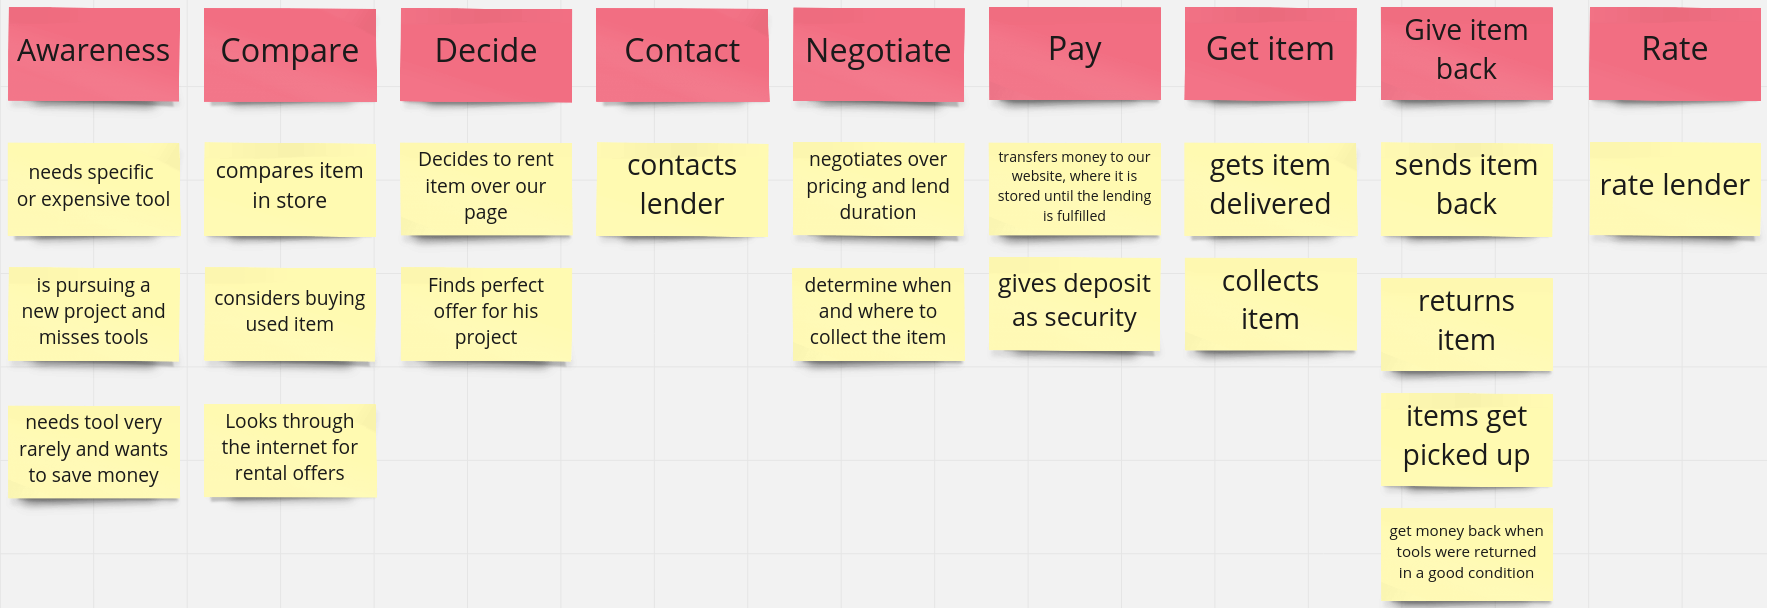
\includegraphics[width=\linewidth]{abb/2_context_of_use/user_journey_map_renting.png}
				\caption{User journey map for renting user}
				\label{fig:ujm_renting}
			\end{figure}
			
			\noindent
			The corresponding feelings and the graph are determined this way:
			
			\begin{figure}[H]
				\centering
				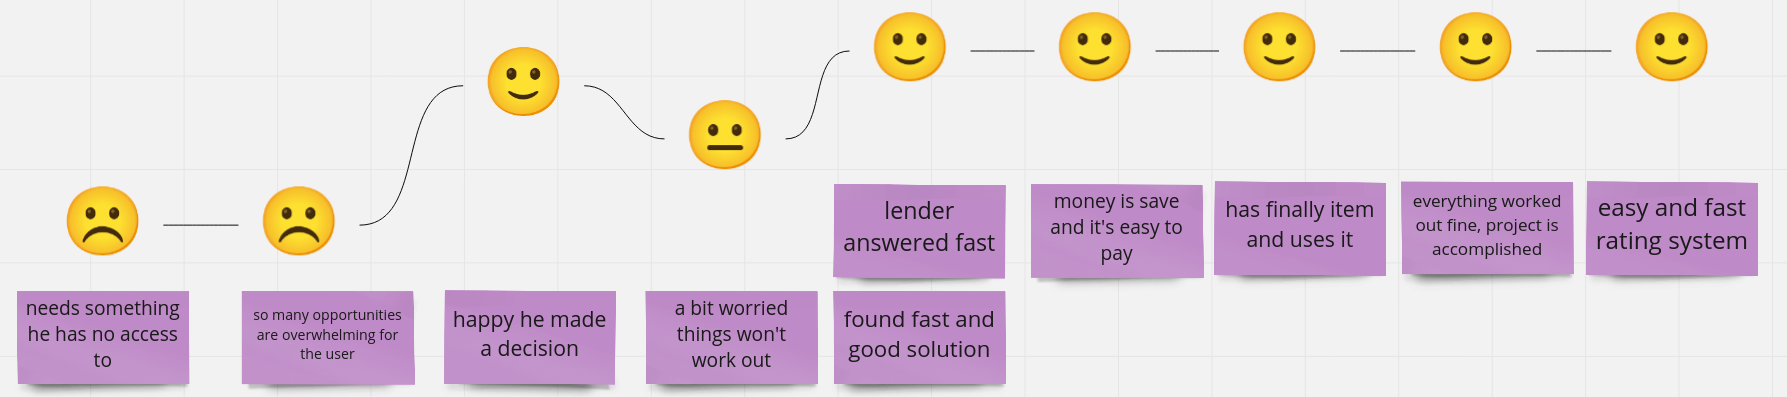
\includegraphics[width=\linewidth]{abb/2_context_of_use/feelings_renting.png}
				\caption{Feelings for renting user}
				\label{fig:ujm_renting_feelings}
			\end{figure}
		
		\subsubsection{User journey map for the renting person}
			The counterparts for the renting persons journey looks like this:
			
			\begin{figure}[H]
				\centering
				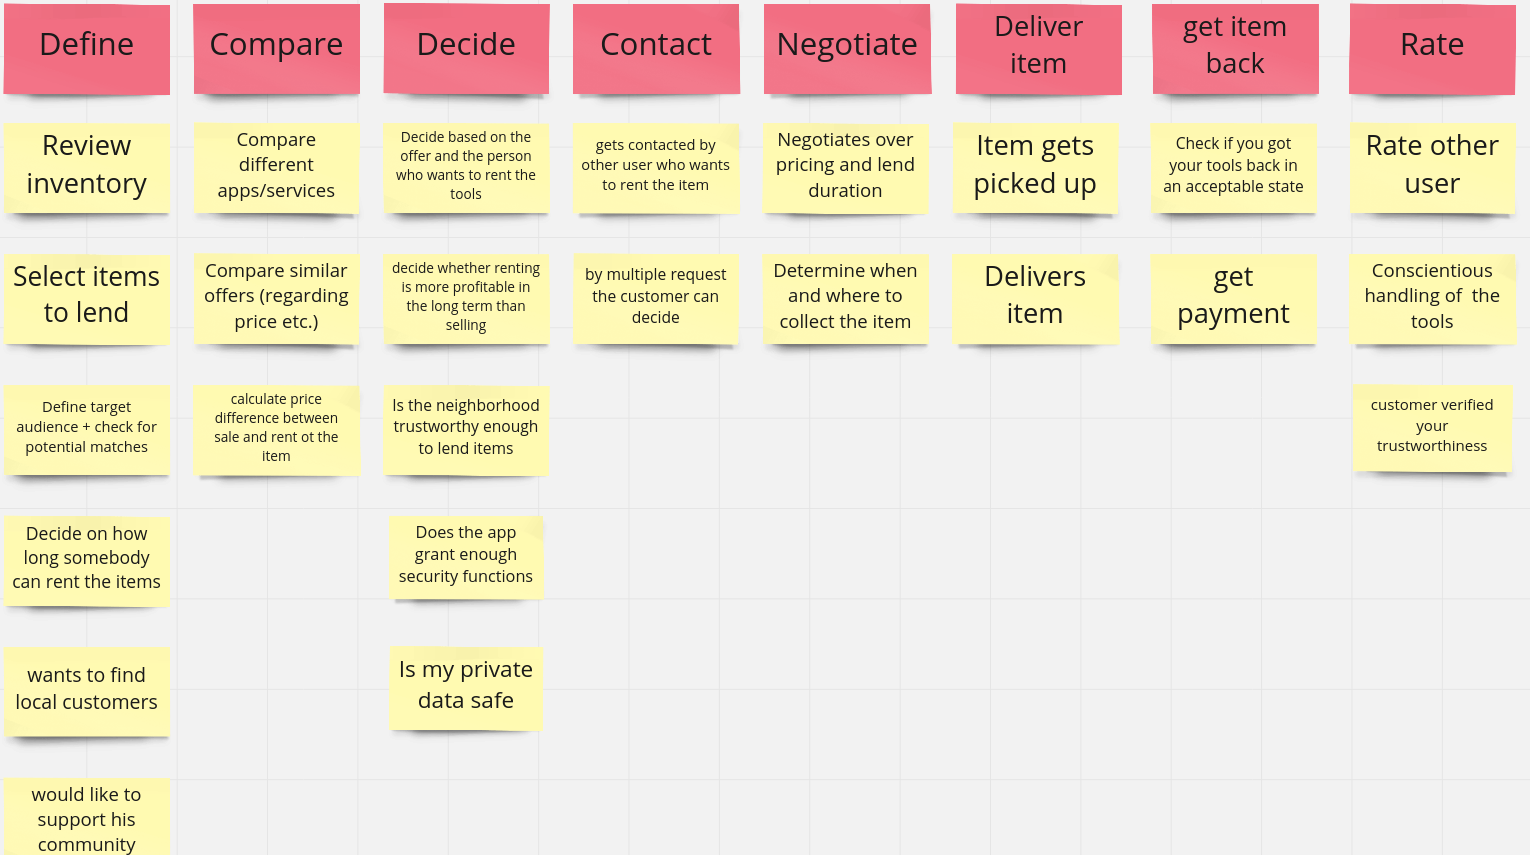
\includegraphics[width=\linewidth]{abb/2_context_of_use/user_journey_map_lending.png}
				\caption{User journey map for lending user}
				\label{fig:ujm_lending}
			\end{figure}
		
			\begin{figure}[H]
				\centering
				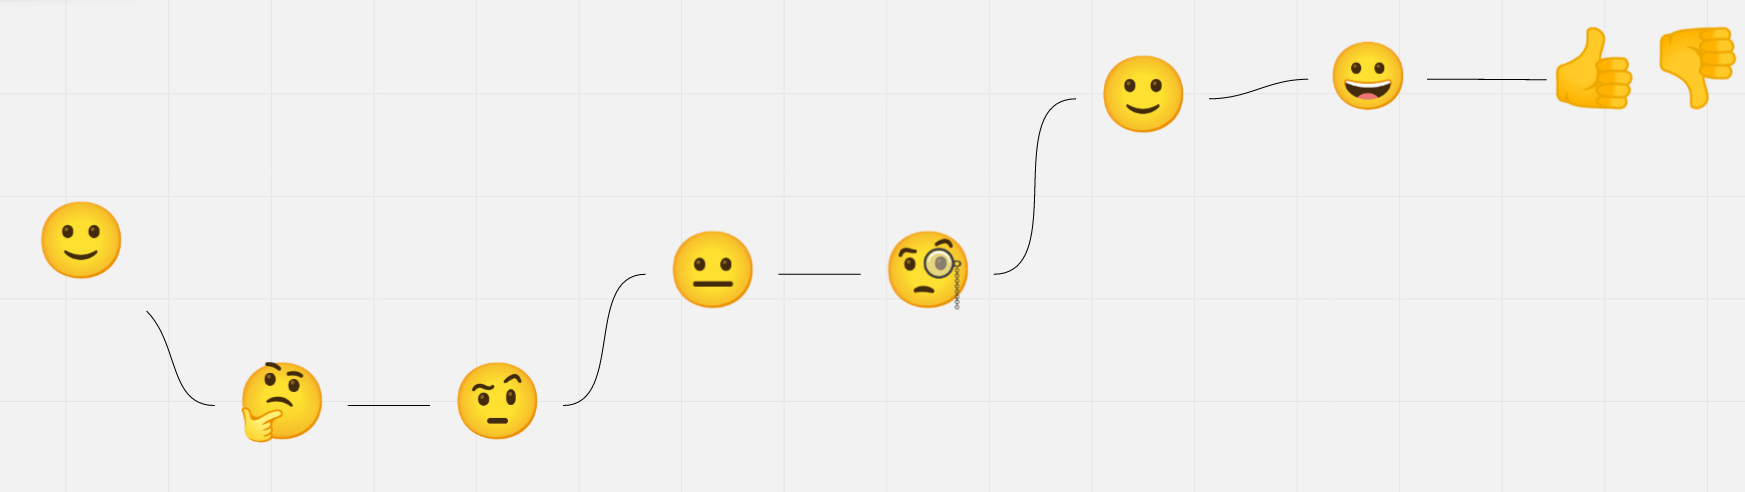
\includegraphics[width=\linewidth]{abb/2_context_of_use/feelings_lending.png}
				\caption{Feelings for renting user}
				\label{fig:ujm_lending_feelings}
			\end{figure}

\subsection{User Stories}

\definecolor{role}{HTML}{fac710}
\definecolor{goal}{HTML}{cee741}
\definecolor{benefit}{HTML}{2D9BF0}

User stories were developed to precisely identify the needs of the users in their roles. To illustrate this, the stories were listed in a mind map. Here, the map can be read from the inside out as follows:\\
\textbf {As a \colorbox{role}{<role>} I want \colorbox{goal}{<goal>} so that \colorbox{benefit}{<benefit>}}\\
The stories are sorted from top to bottom by importance.

\subsubsection{Stories for the renter}
\begin{figure}[H]
	\centering
	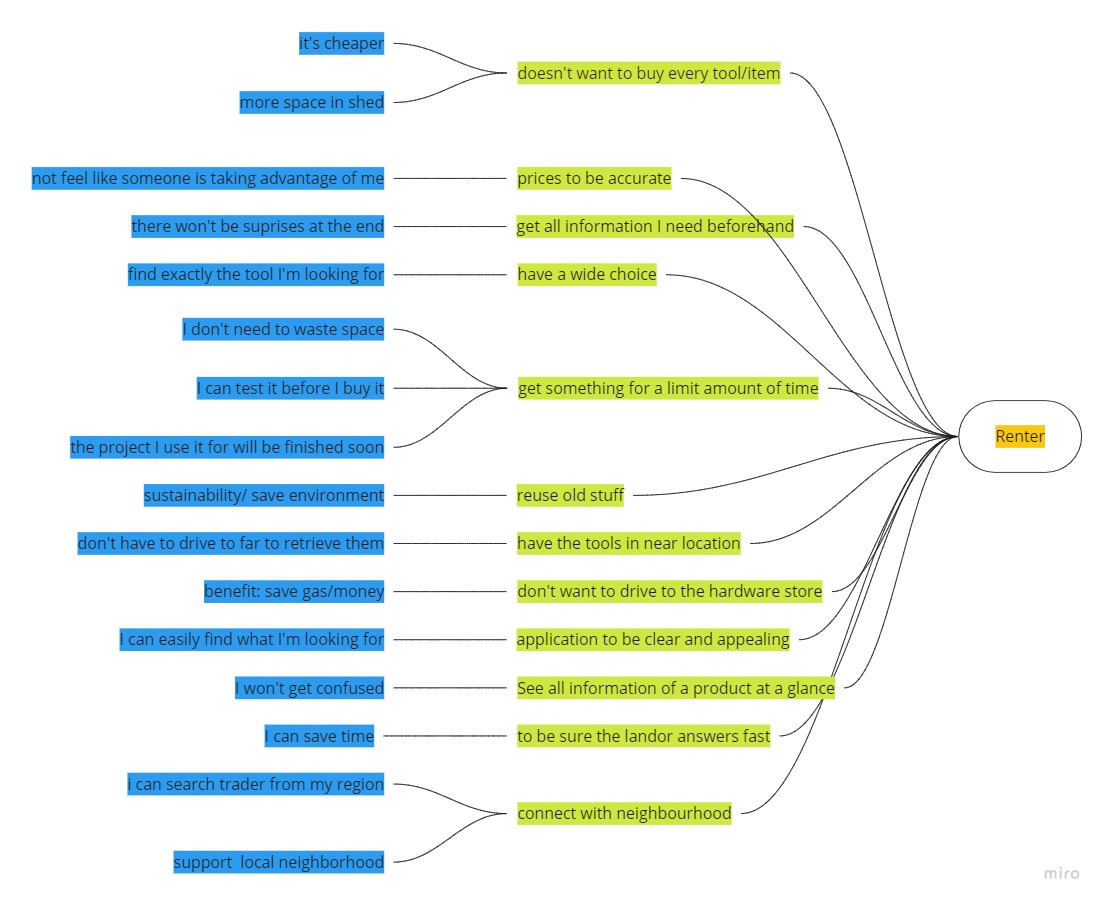
\includegraphics[width=\linewidth]{abb/2_context_of_use/story_renting.jpg}
	\caption{Renter Story}
	\label{fig:story_renter}
\end{figure}


\subsubsection{Stories for the lender}
\begin{figure}[H]
	\centering
	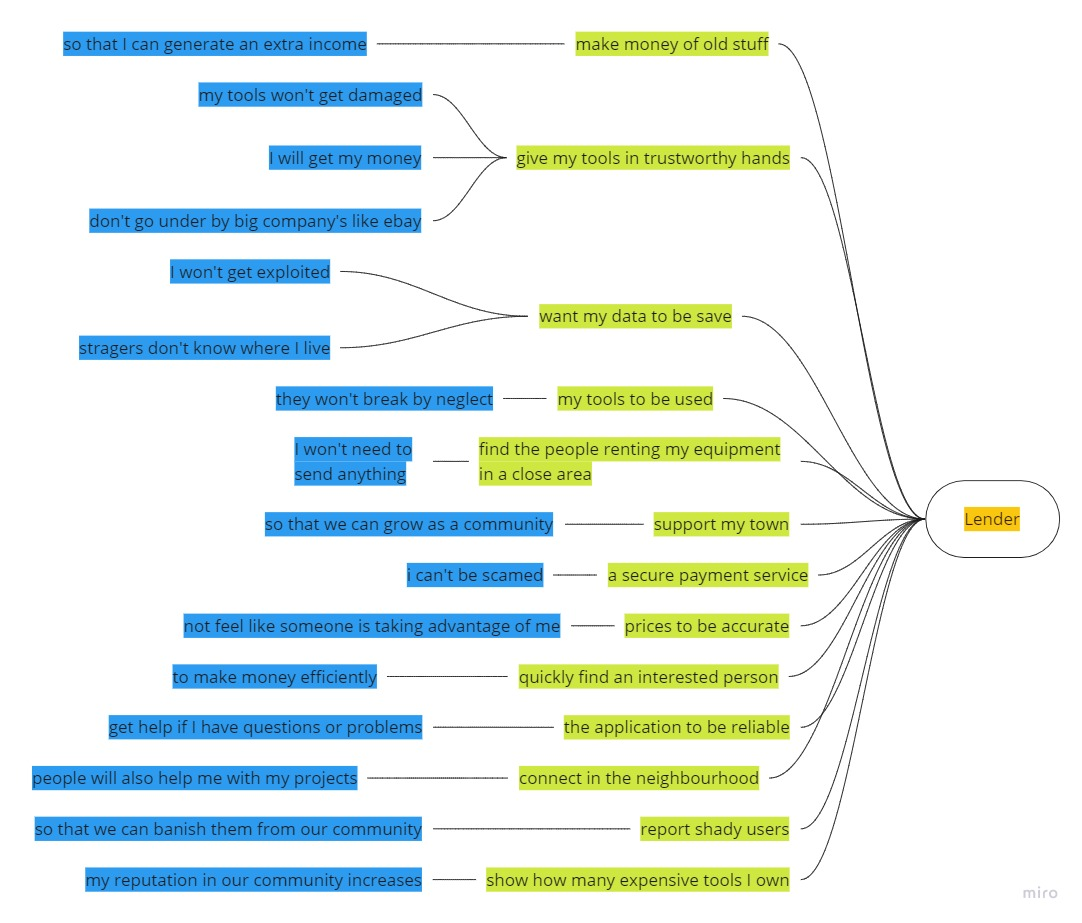
\includegraphics[width=\linewidth]{abb/2_context_of_use/story_lending.jpg}
	\caption{Lender Story}
	\label{fig:story_lender}
\end{figure}


	\newpage
	\section{Design Guidelines}
	In order to create an application with a simple to understand and familiar design, design patterns are used in the later prototyping process. The following design patterns are considered useful after a session of brainstorming:
	
	\begin{itemize}
		\item Steps Left Pattern
		\item Cards Pattern
		\item Autocomplete	
		\item Input Feedback Pattern
		\item Rate Content Pattern
		\item Chat Pattern
		\item Product Page Pattern
		\item Gallery Pattern
		\item Calendar Picker Pattern
		\item Password Strength Meter Pattern
		\item Dashboard Pattern
		\item Status-Quo Bias Pattern
		\item Chunking Pattern
		\item Main Navigation
		\item Shortcut Dropdown
		
		% nicht umgesetzt
		\item Preview Pattern
		\item Flagging \& Reporting Pattern
		\item Categorization Pattern
		\item Personalized "My Site"
		\item Pay to Promote Pattern
		\item Reduction Pattern
	\end{itemize}

	\paragraph{Steps Left}
		This pattern is used when both lending and renting parties are communicating via the chat. A overview of already completed and pending steps is displayed next to the chat window.
		
		\begin{figure}[H]
			\centering
			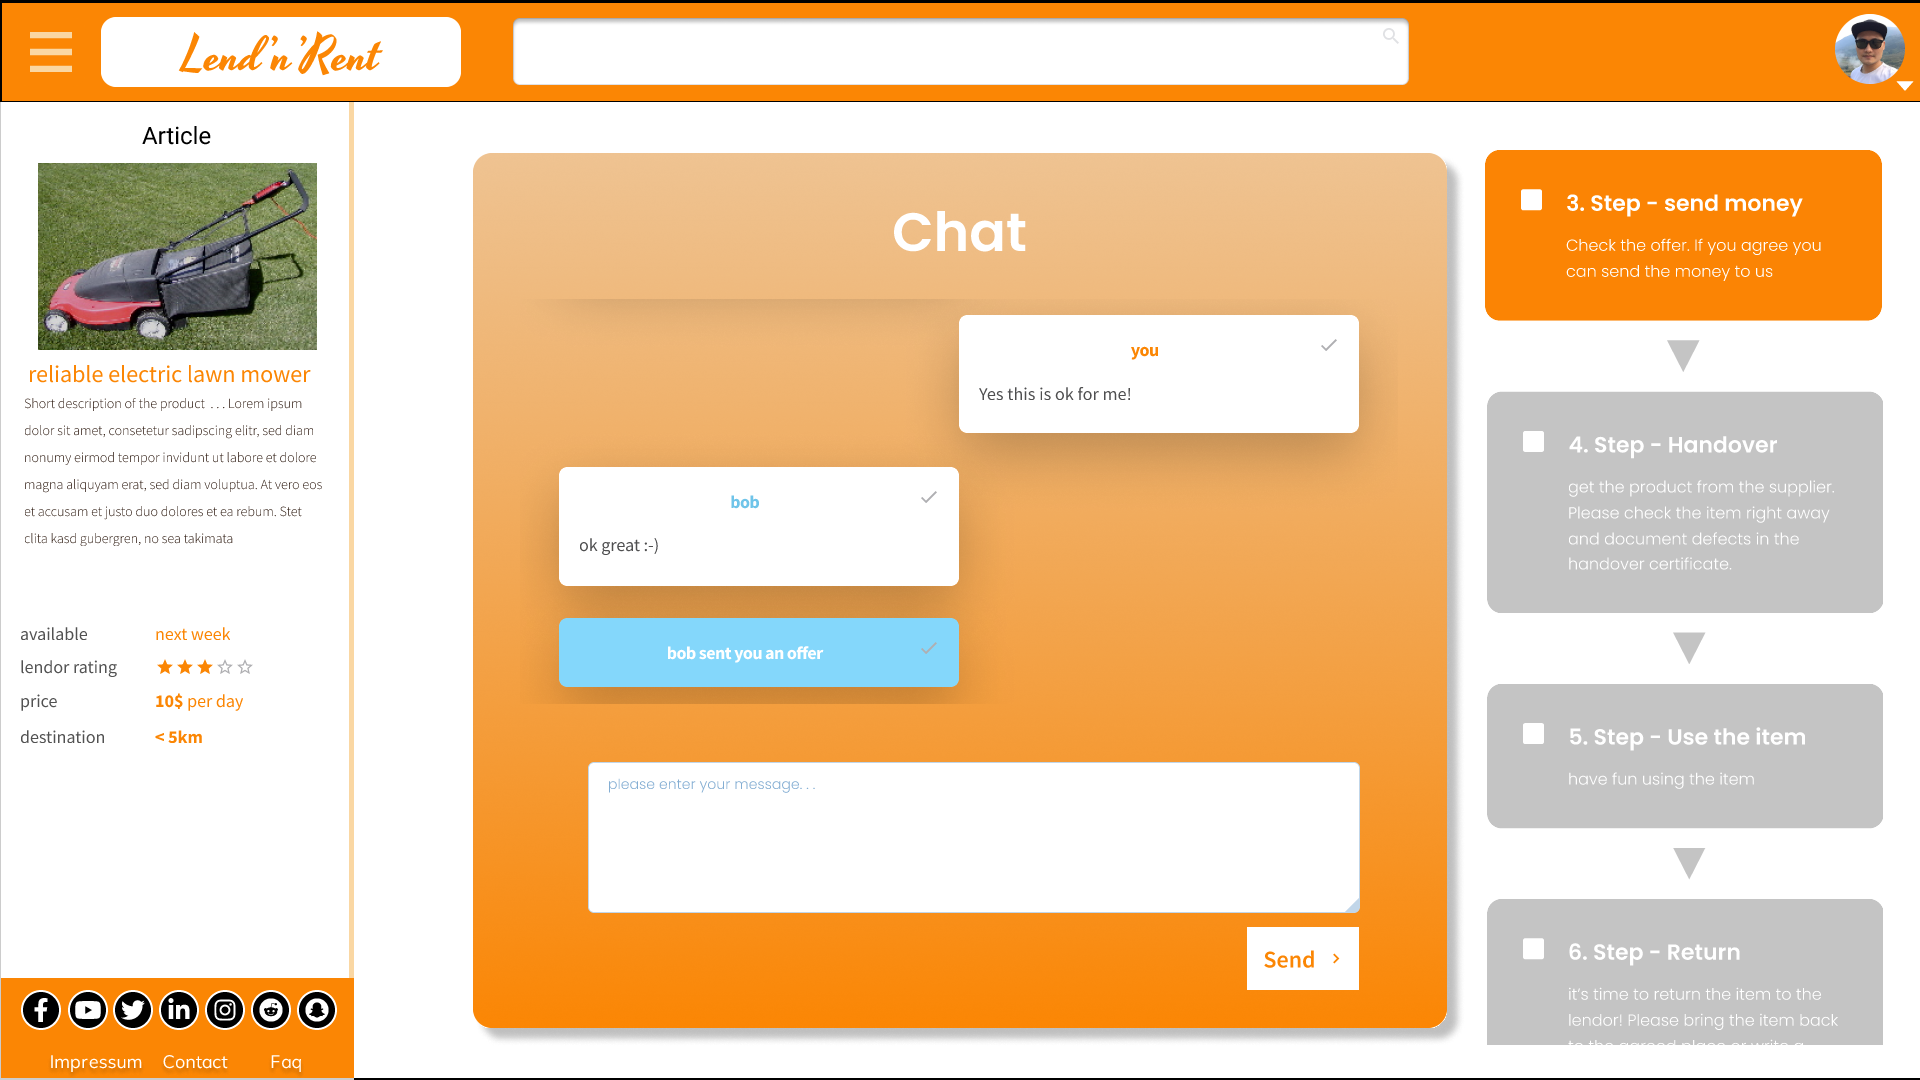
\includegraphics[width=\linewidth]{abb/3_design_guidelines/stepsleft.png}
			\caption{Steps Left pattern next to the chat window}
			\label{fig:stepsleft}
		\end{figure}
	\par
	
	\paragraph{Cards}
		Every offer as well as advertisements in the offer detail page is placed within a separate card including a picture of the item, the description, the price per day, the proximity to the users location and when it is available. With this pattern each offer can be distinguished from the other offers at the first glance.
		
		\begin{figure}[H]
			\centering
			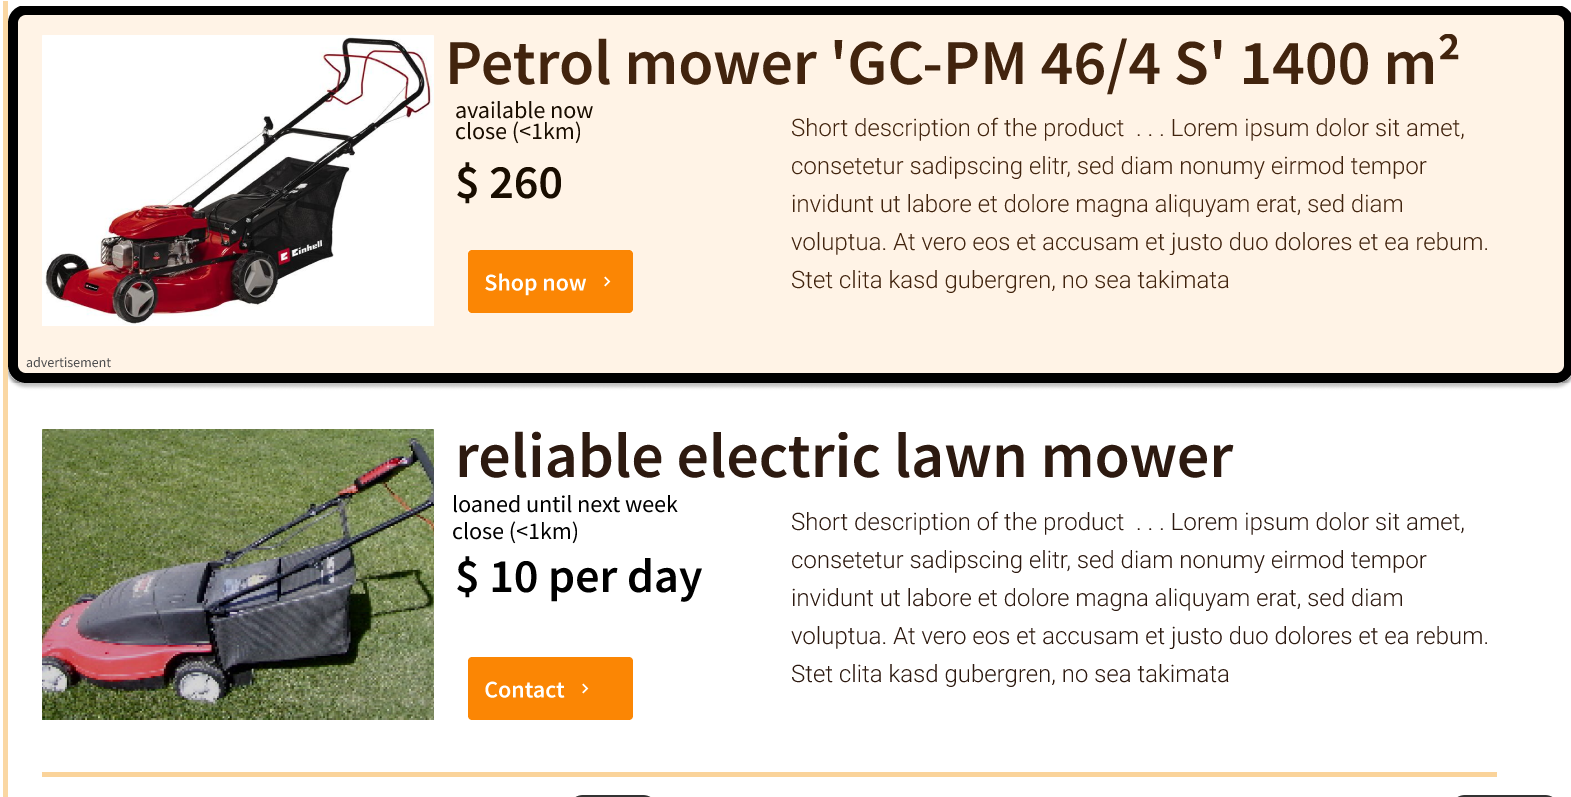
\includegraphics[width=\linewidth]{abb/3_design_guidelines/cards.png}
			\caption{Offer and advertisement cards}
			\label{fig:cards}
		\end{figure}
	\par
	
	\paragraph{Autocomplete and Input Feedback}
		These patterns are used when searching for items and editing the profile. The search query in the search bar and the users address will have suggestions for autocompletion based on previous queries and location services. The inputs will be validated and will have a green tick mark if the format is correct.
	\par
	
	\paragraph{Rate Content}
		When the item is returned after it has been used, both parties can rate each others trustworthiness. This helps future parties to decide if they can trust this user when borrowing from the user or lending to them. This rating takes place in the chat window as a part of the steps to complete the deal.
		
		\begin{figure}[H]
			\centering
			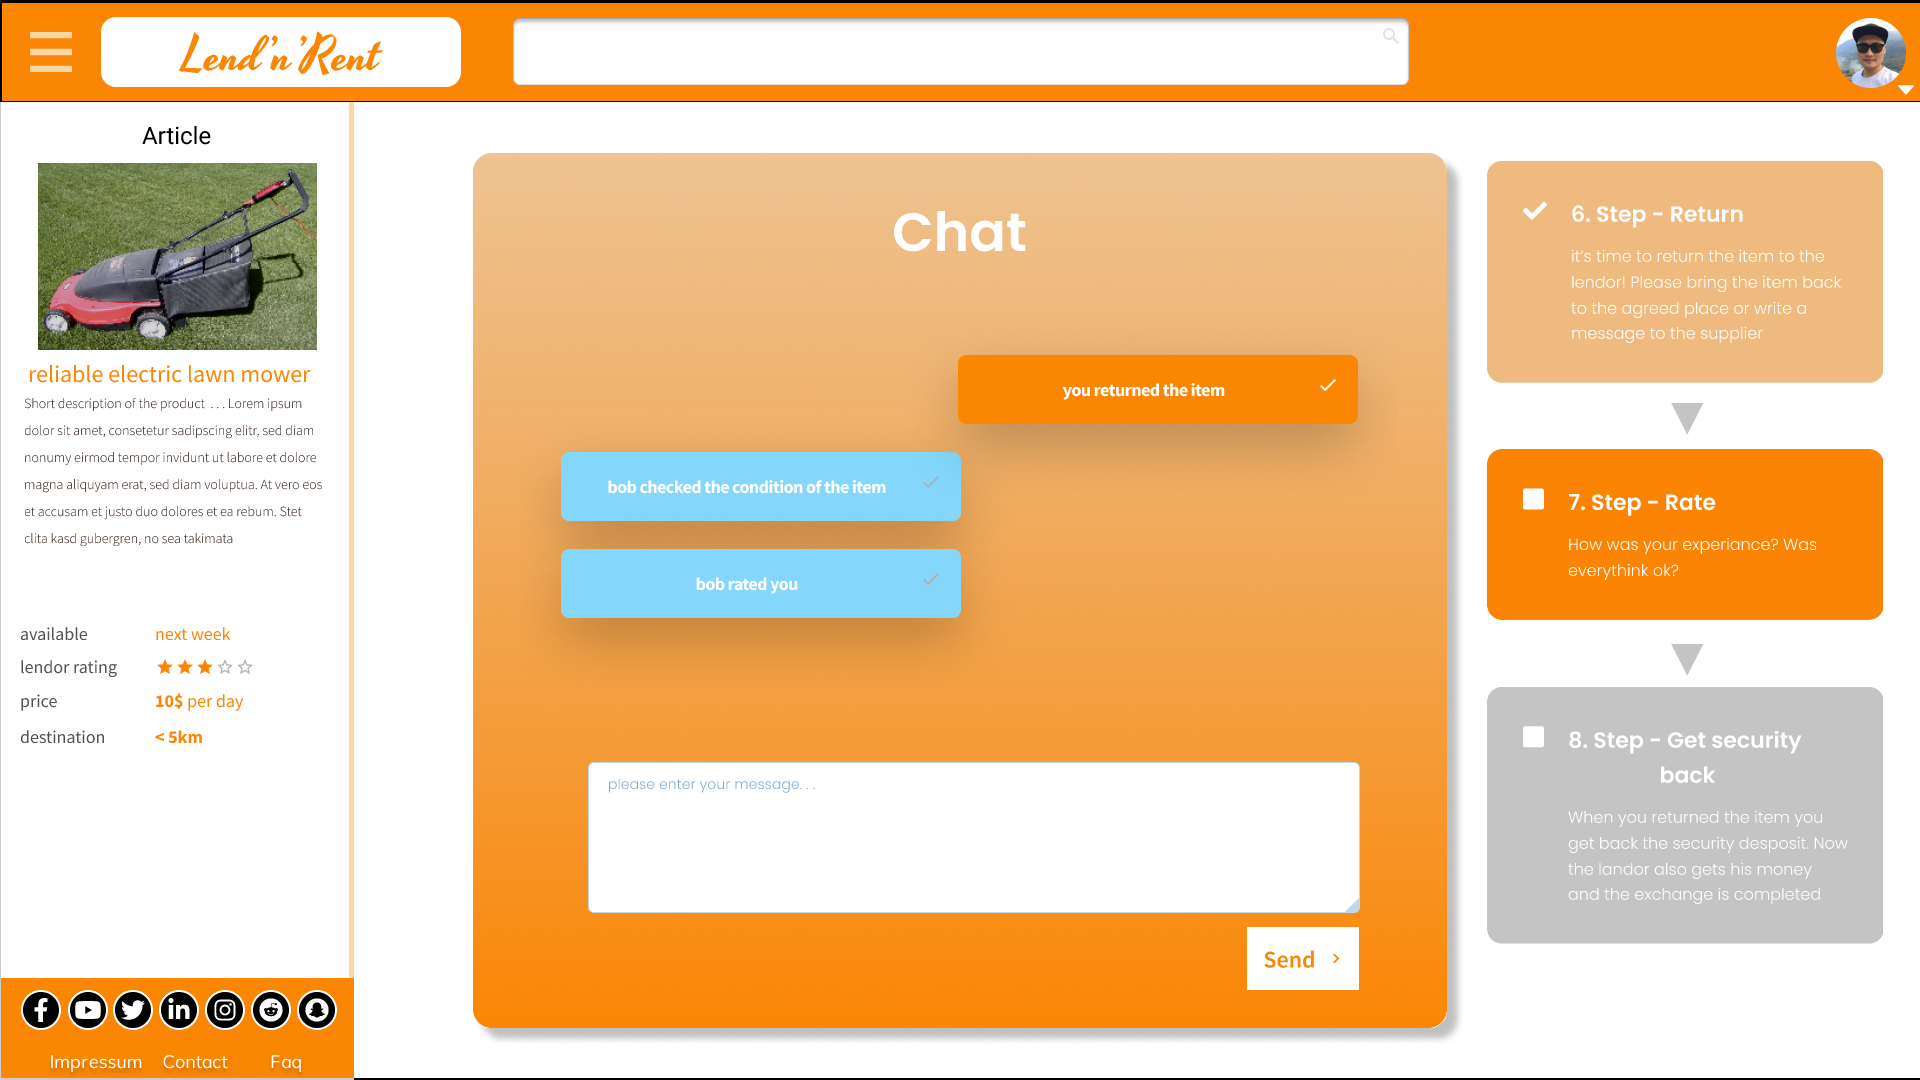
\includegraphics[width=\linewidth]{abb/3_design_guidelines/rate.png}
			\caption{Rating the users}
			\label{fig:rate}
		\end{figure}
	\par
	
	\paragraph{Chat}
		The Chat is the main tool for communication between the lending and renting parties. It is used to 
		\begin{itemize}
			\item contact the lender
			\item agree on the terms of price, deposit and duration
			\item initiate the transfer of money
			\item rate the other party
		\end{itemize}
	\par
	
	\paragraph{Product Page}
		At the product page the user can read the description, contact the lender, see the price, availability and proximity at one glance.
	\par
	
	\paragraph{Gallery}
		Galleries are used on the product detail page when the lender uploads more than one picture for their item. This is used to prevent that all images appear at once and overwhelm the user. It also adds structure to the page.
	\par
	
	\paragraph{Calendar Picker}
		When the lender adds a new offer, they can pick a date to that the item is available for borrowing. The calendar picker appears after clicking the icon next to the input field. This adds comfort for the user because they do not have to enter the date manually and have a visual representation of the weeks.
		
		\begin{figure}[H]
			\centering
			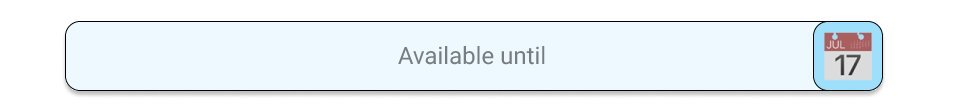
\includegraphics[width=\linewidth]{abb/3_design_guidelines/calendar_picker.png}
			\caption{Calendar picker}
			\label{fig:calendar_picker}
		\end{figure}
	\par
	
	\paragraph{Password Strength Meter}
		When a user creates a new account or changes their current password, the password strength meter will indicated how secure the new chosen password is.
	\par
	
	\paragraph{Dashboard}
		The overview of all messages has certain dashboard functionalities. The user can see all of their incoming and outgoing messages and navigate into the different chat rooms. The incoming and outgoing messages are separated into two tabs.
		\begin{figure}[H]
			\centering
			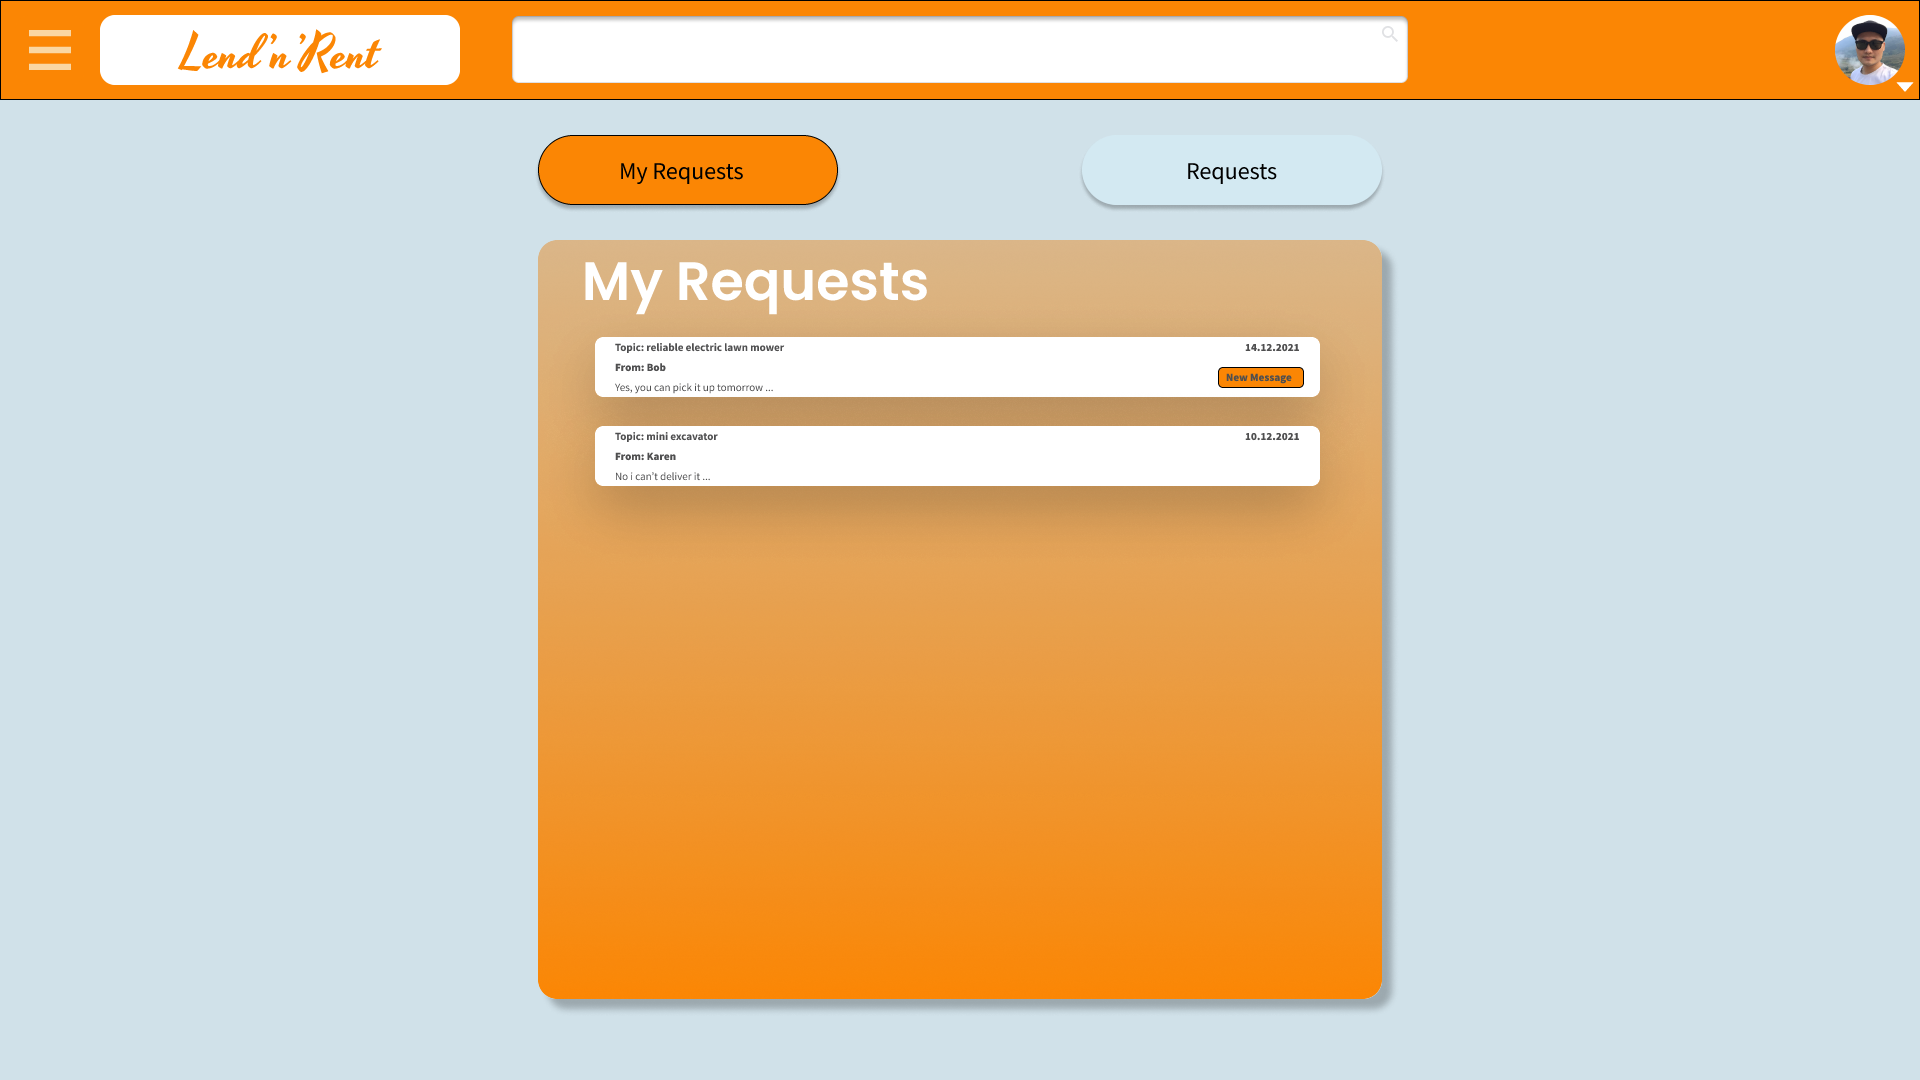
\includegraphics[width=0.49\linewidth]{abb/3_design_guidelines/messages_1.png}
			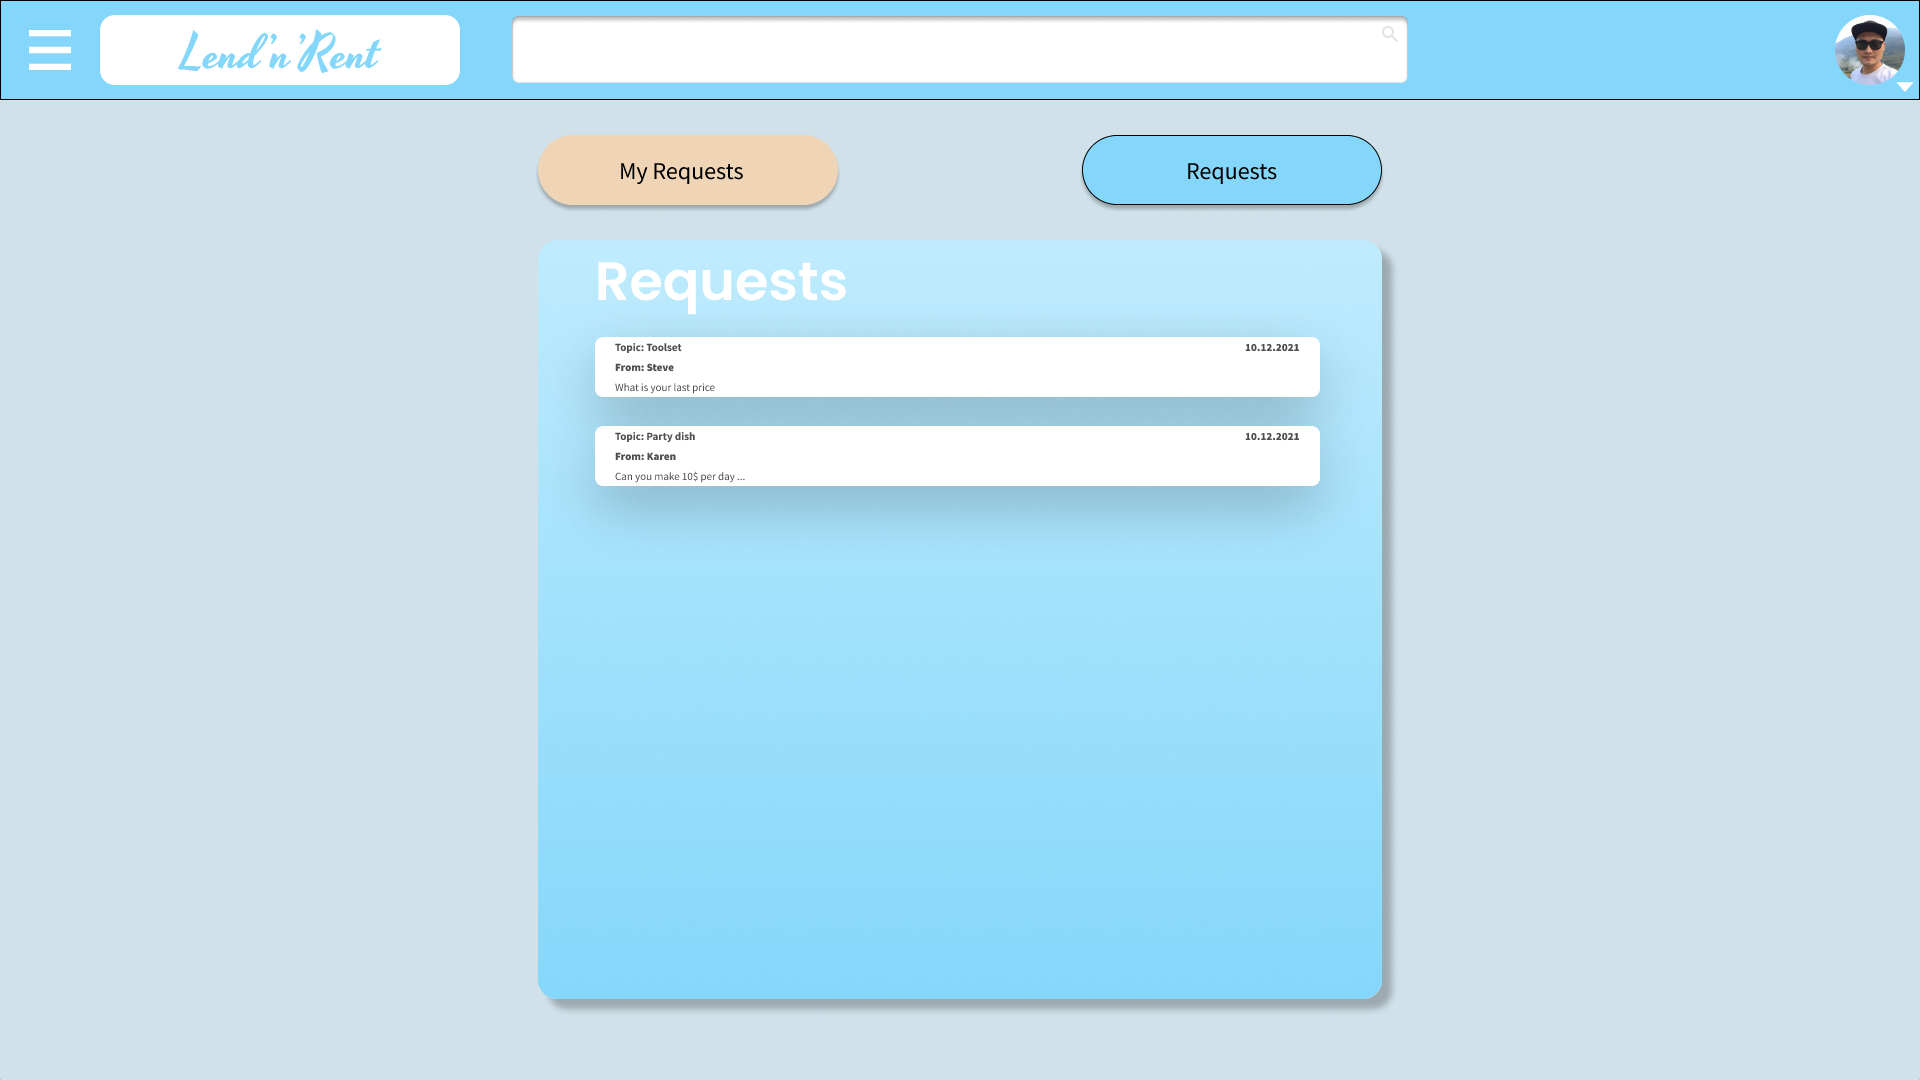
\includegraphics[width=0.49\linewidth]{abb/3_design_guidelines/messages_2.png}
			\caption{Message dashboard}
			\label{fig:message_dashboard}
		\end{figure}
	\par
	
	\paragraph{Status-Quo Bias}
		The landing pages color scheme is set to orange that signals the user that they are using the borrowing part of the plattform. This decision was made because most of the time the users probably want to search for items and compare them with their needs. The assumption that was made is that only more experienced users want to offer their items for borrowing.
	\par
	
	\paragraph{Shortcut Dropdown}
		The user can filter their search results by category either by navigating through a tree of submenus or by using a dropdown menu above the search results.
		\begin{figure}[H]
			\centering
			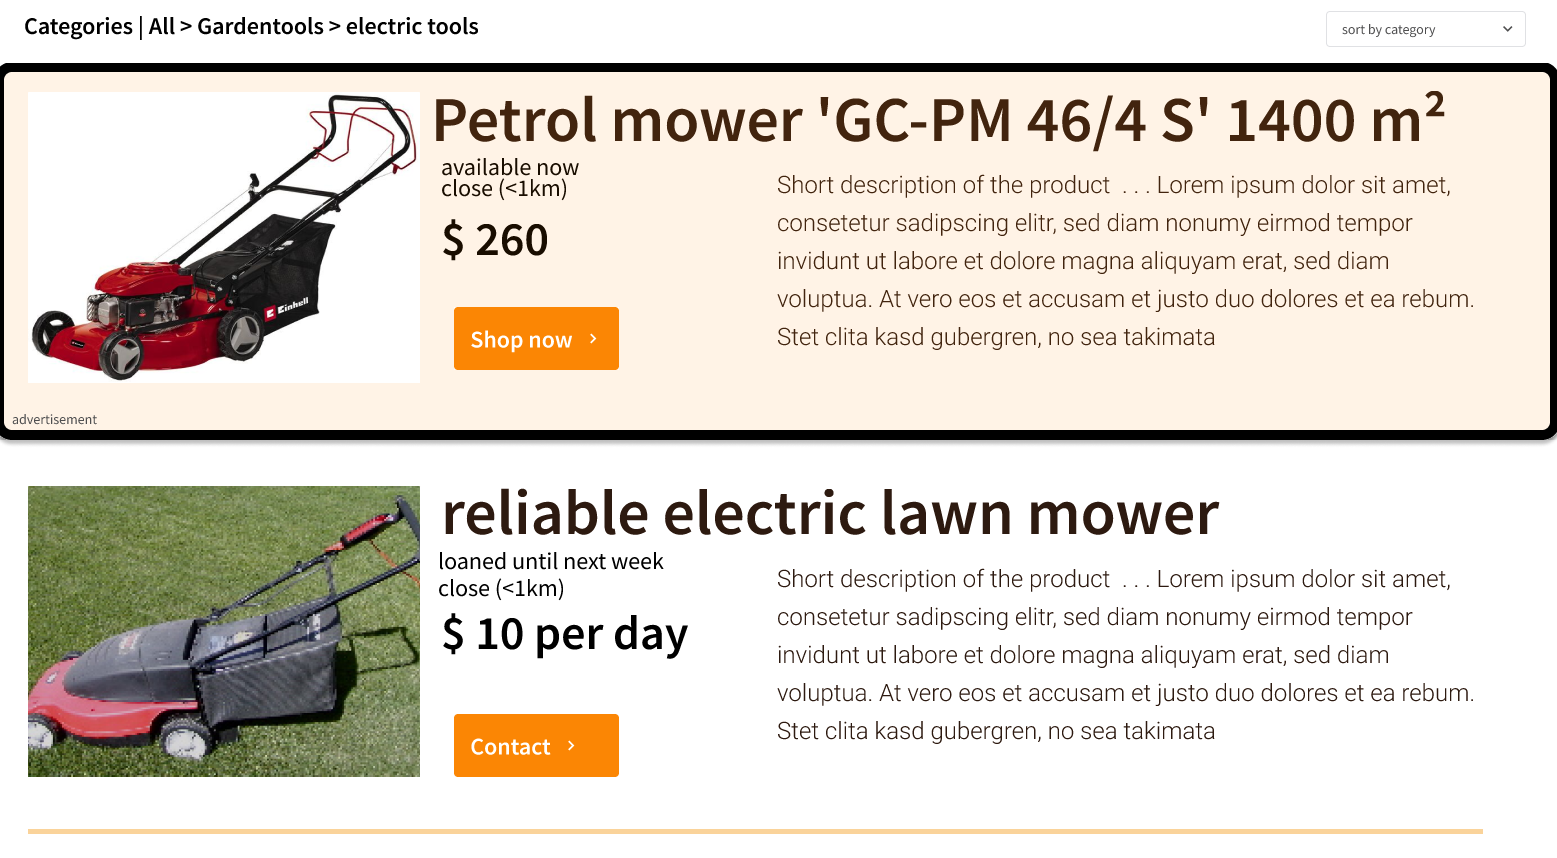
\includegraphics[width=\linewidth]{abb/3_design_guidelines/dropdown_shortcut.png}
			\caption{Dropdown Shortcut}
			\label{fig:dropdown_shortcut}
		\end{figure}
	\par
	
	
	
	
	\newpage
	\section{Information Architecture}
	\newpage
	\section{Competitive Analysis}
	\newpage
	\section{Sketching and Paper Prototyping}

    \subsection{Sketching}
        For Sketching our team met every Monday and Tuesday to discuss our ideas. Everyone had time to present and the opportunity to share their ideas with the team. After that, we discussed the pros and cons of the ideas and decided which functionalities and aspects we can include in our project.
        
    \subsection{Paper Prototyping}
        For the first draft of the landing page we did a paper prototype. We used some elements from this first draft to design our layout for Lend'n'Rent.
        
        	\begin{figure}[H]
				\centering
				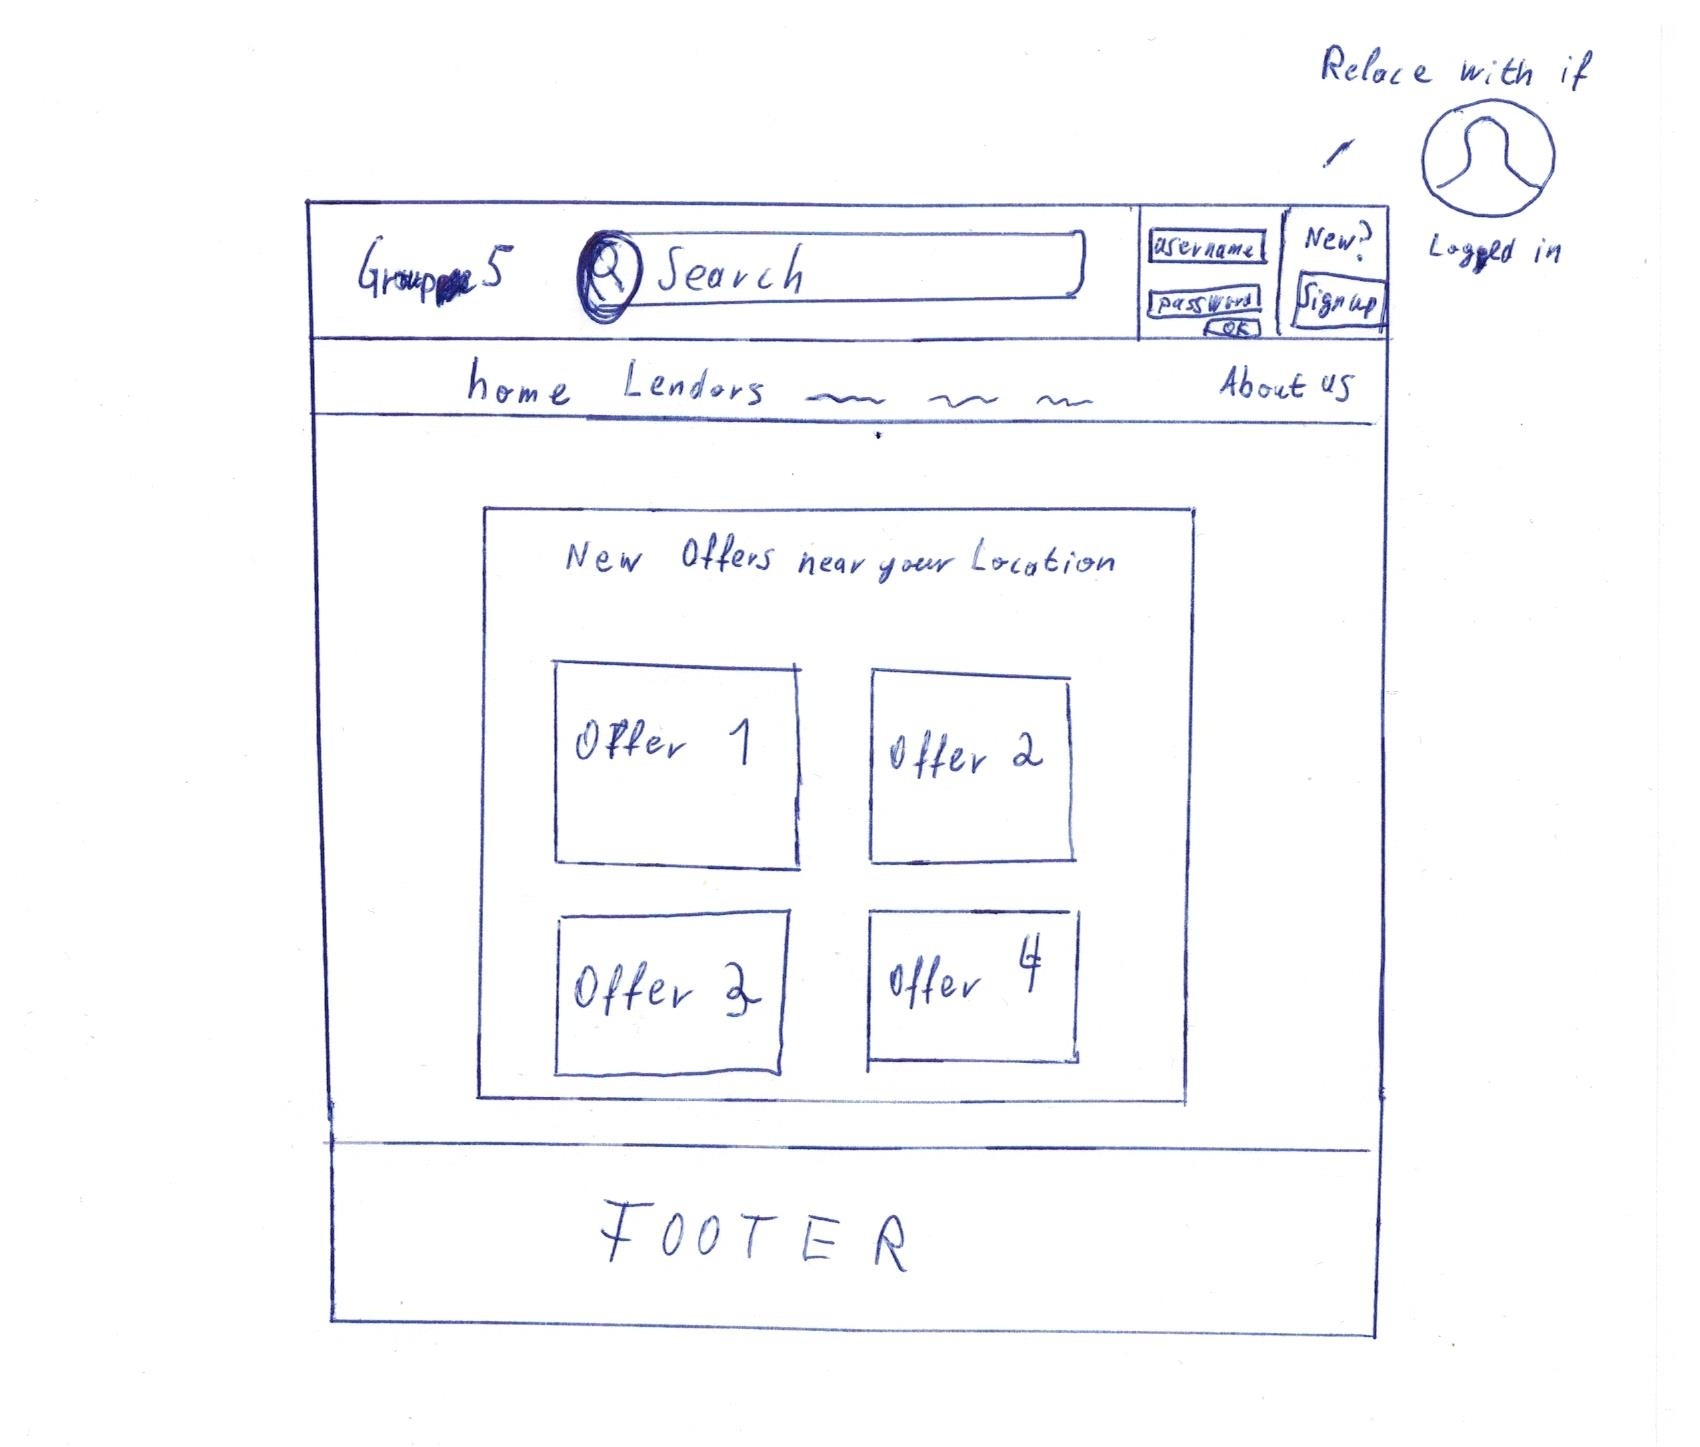
\includegraphics[width=\linewidth]{abb/6_Sketching and Paper Prototyping/Homepage1.png}
				\caption{Landing Page Paper Prototype 1}
				\label{fig:Homepage1}
			\end{figure}
			
			\noindent
			From the first paper prototype we adopt that the search bar and the profile picture are included in the navigation bar on top of the website. We incorporated the offers into the categories page. 
			
			
			 \begin{figure}[H]
				\centering
				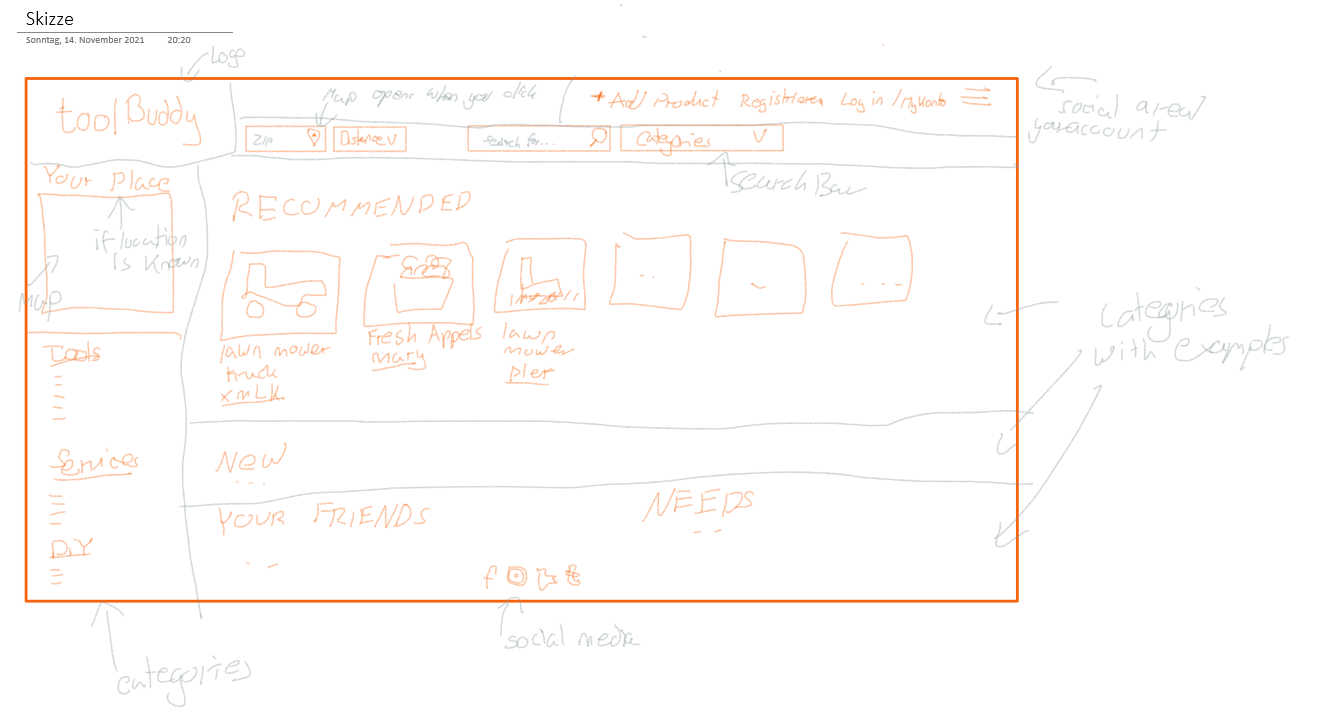
\includegraphics[width=\linewidth]{abb/6_Sketching and Paper Prototyping/Homepage2.png}
				\caption{Landing Page Paper Landing Page 2}
				\label{fig:Homepage2}
			\end{figure}
			
			\noindent
			From prototype 2 we adopted the left sidebar for the majority of our page flow including the functionality to use a map to look for tools around your area instead of using a formula where you need to type your location.
			
			\begin{figure}[H]
				\centering
				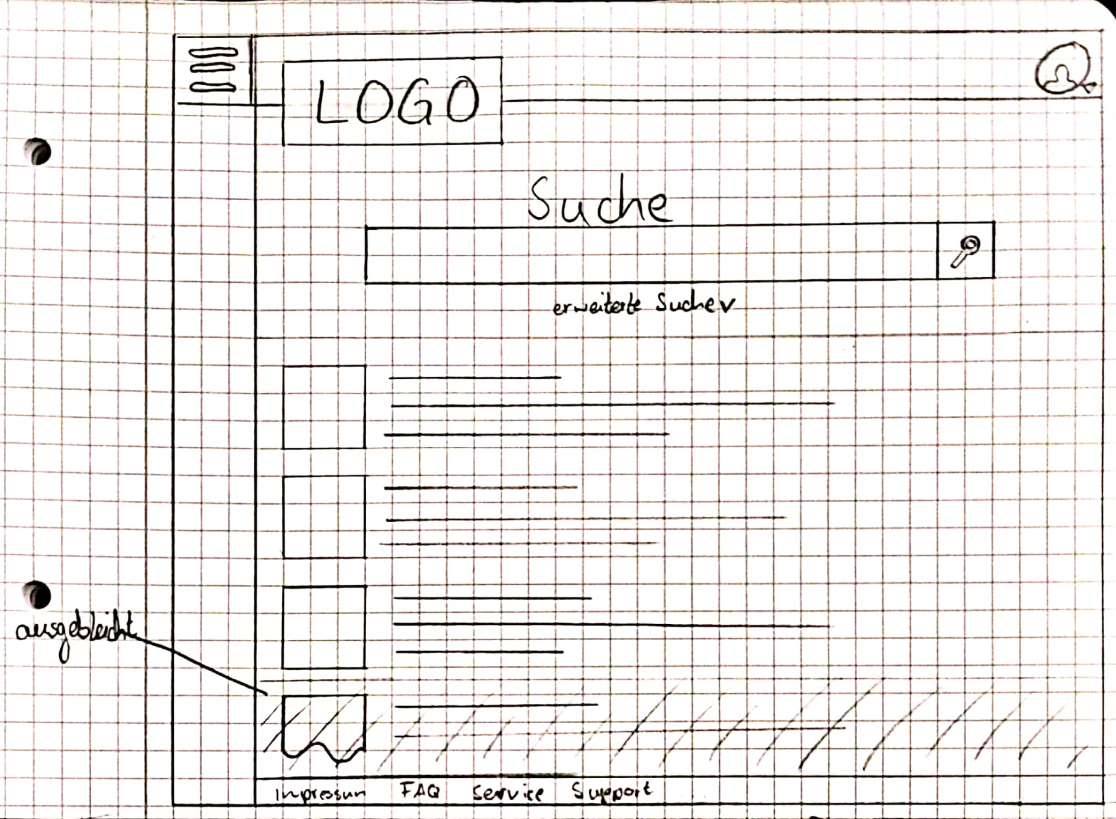
\includegraphics[width=\linewidth]{abb/6_Sketching and Paper Prototyping/Homepage3.png}
				\caption{Landing Page Paper Prototype 3.1}
				\label{fig:Homepage3}
			\end{figure}
			
			
			\begin{figure}[H]
				\centering
				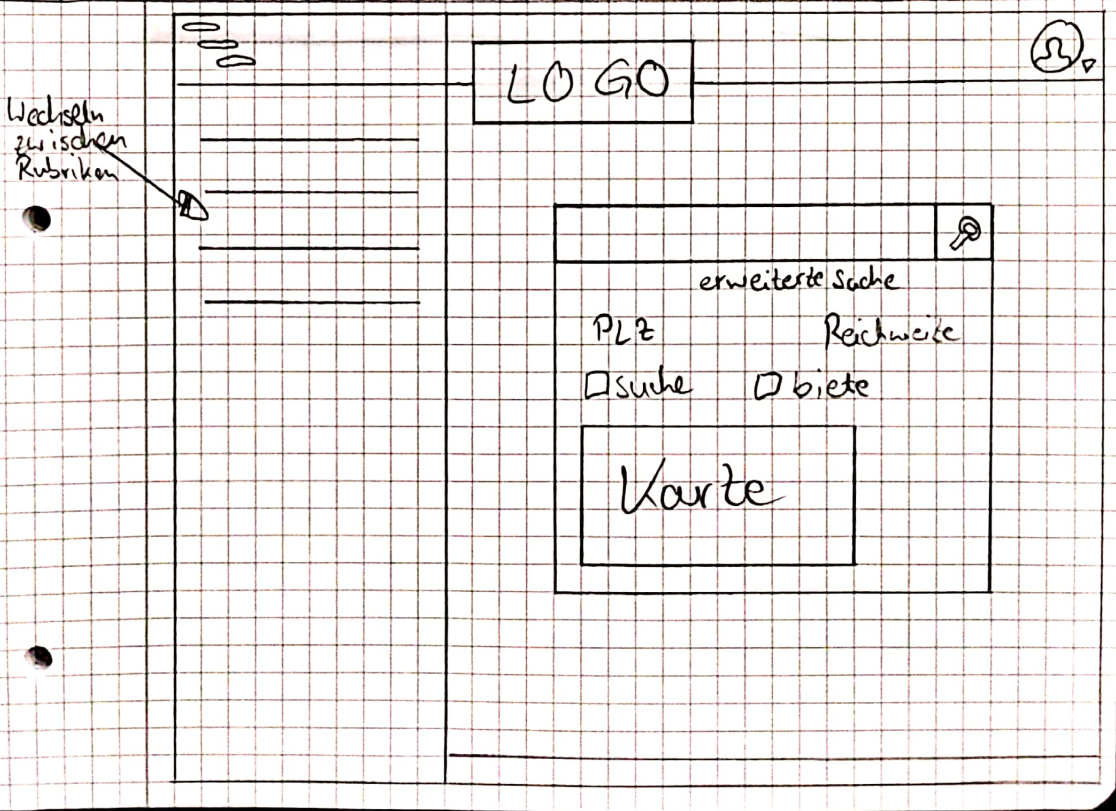
\includegraphics[width=0.9\linewidth]{abb/6_Sketching and Paper Prototyping/Homepage4.png}
				\caption{Landing Page Paper Prototype 3.2}
				\label{fig:Homepage4}
			\end{figure}
			
			\noindent
			From the prototype 4 we decided to use the arrow under the profile picture to allow user to open a drop down menu for easier navigation.
			
			\begin{figure}[H]
				\centering
				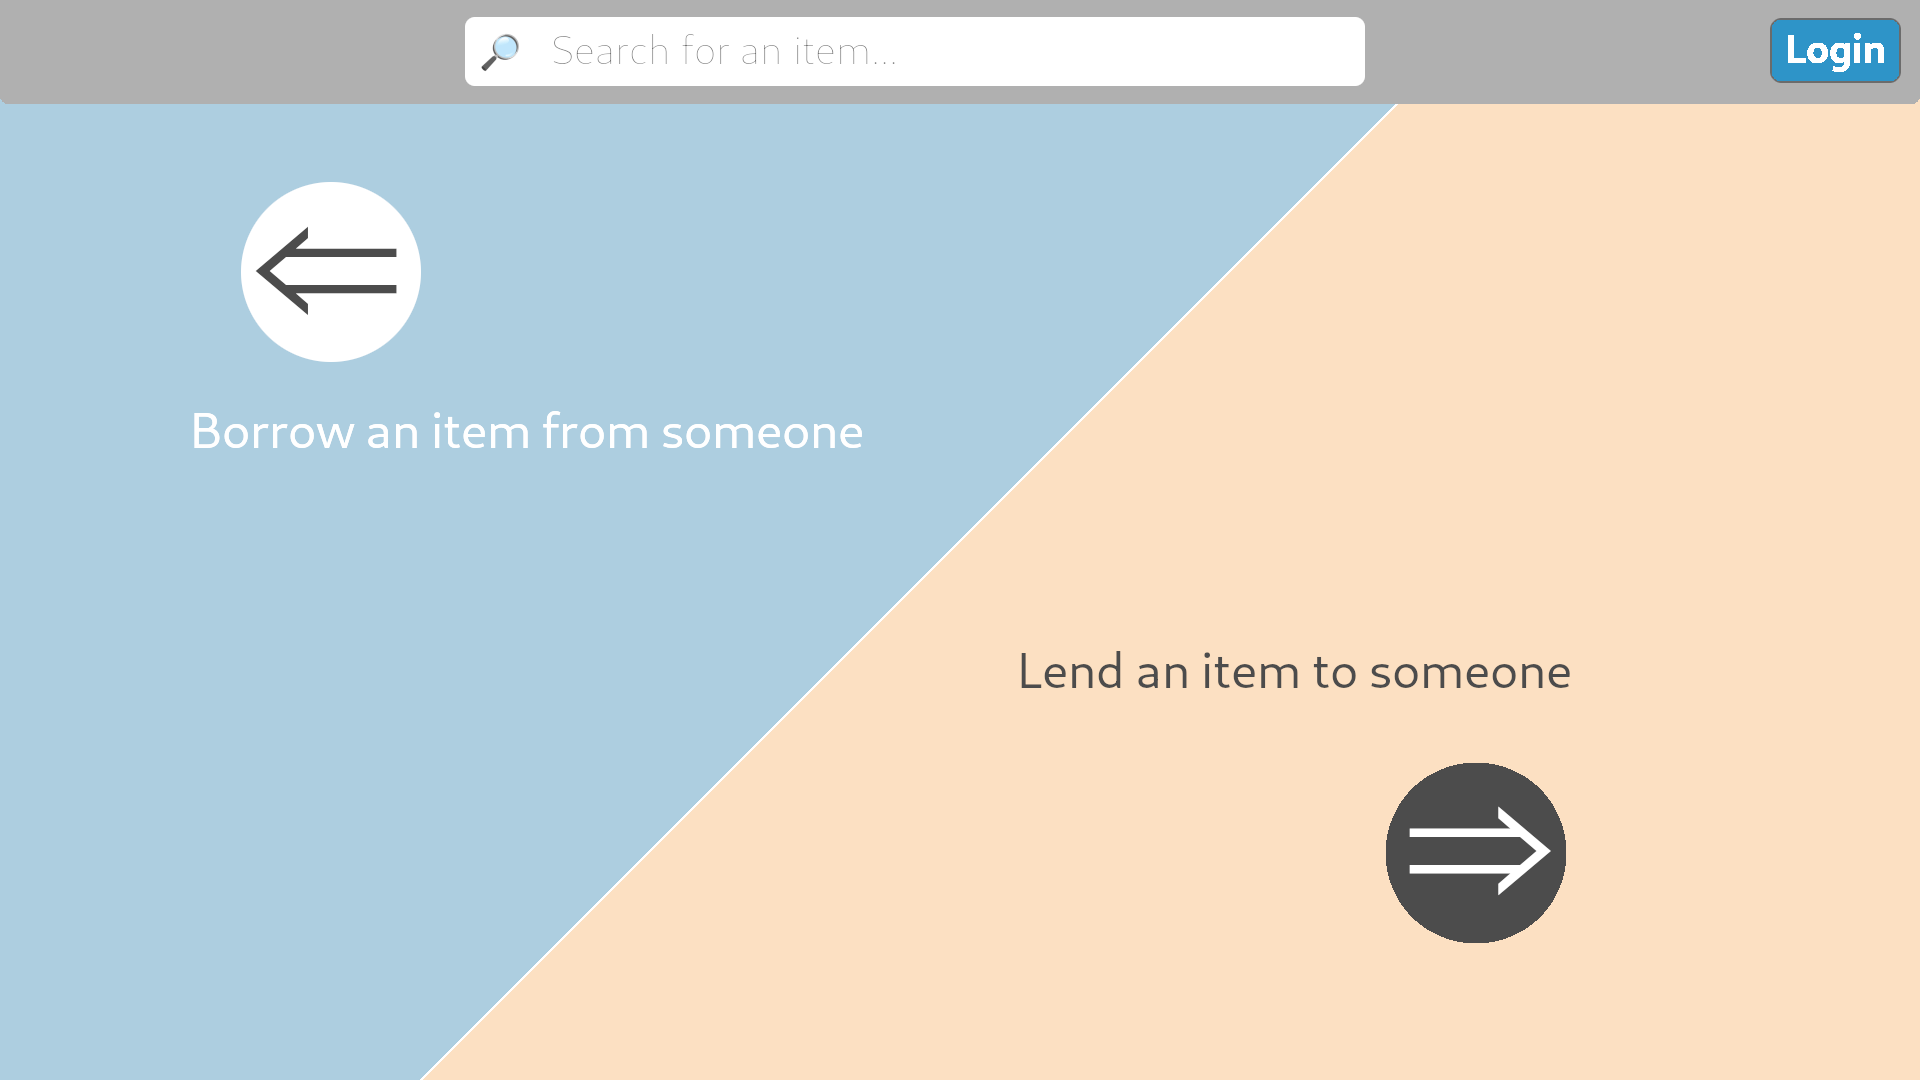
\includegraphics[width=\linewidth]{abb/6_Sketching and Paper Prototyping/Homepage5.png}
				\caption{Landing Page Paper Prototype 4}
				\label{fig:Homepage4}
			\end{figure}
			
			\noindent
			This prototype shows our idea to separate our page flow for our two user groups: Lender and Renter.
			
	\newpage
	\section{Prototyping}

The prototype development was done with Figma and is available at the following link: \\ \url{https://www.figma.com/proto/Ws8rKV3H7ABW2wMOwyFcfj/Lend-n-Rent?node-id=102%3A17674&scaling=min-zoom&page-id=96%3A14807&starting-point-node-id=102%3A17674}

\noindent
Once on the landing page, the user can choose whether to borrow or lend an item by clicking on the relevant page.

\begin{figure}[H]
	\centering
	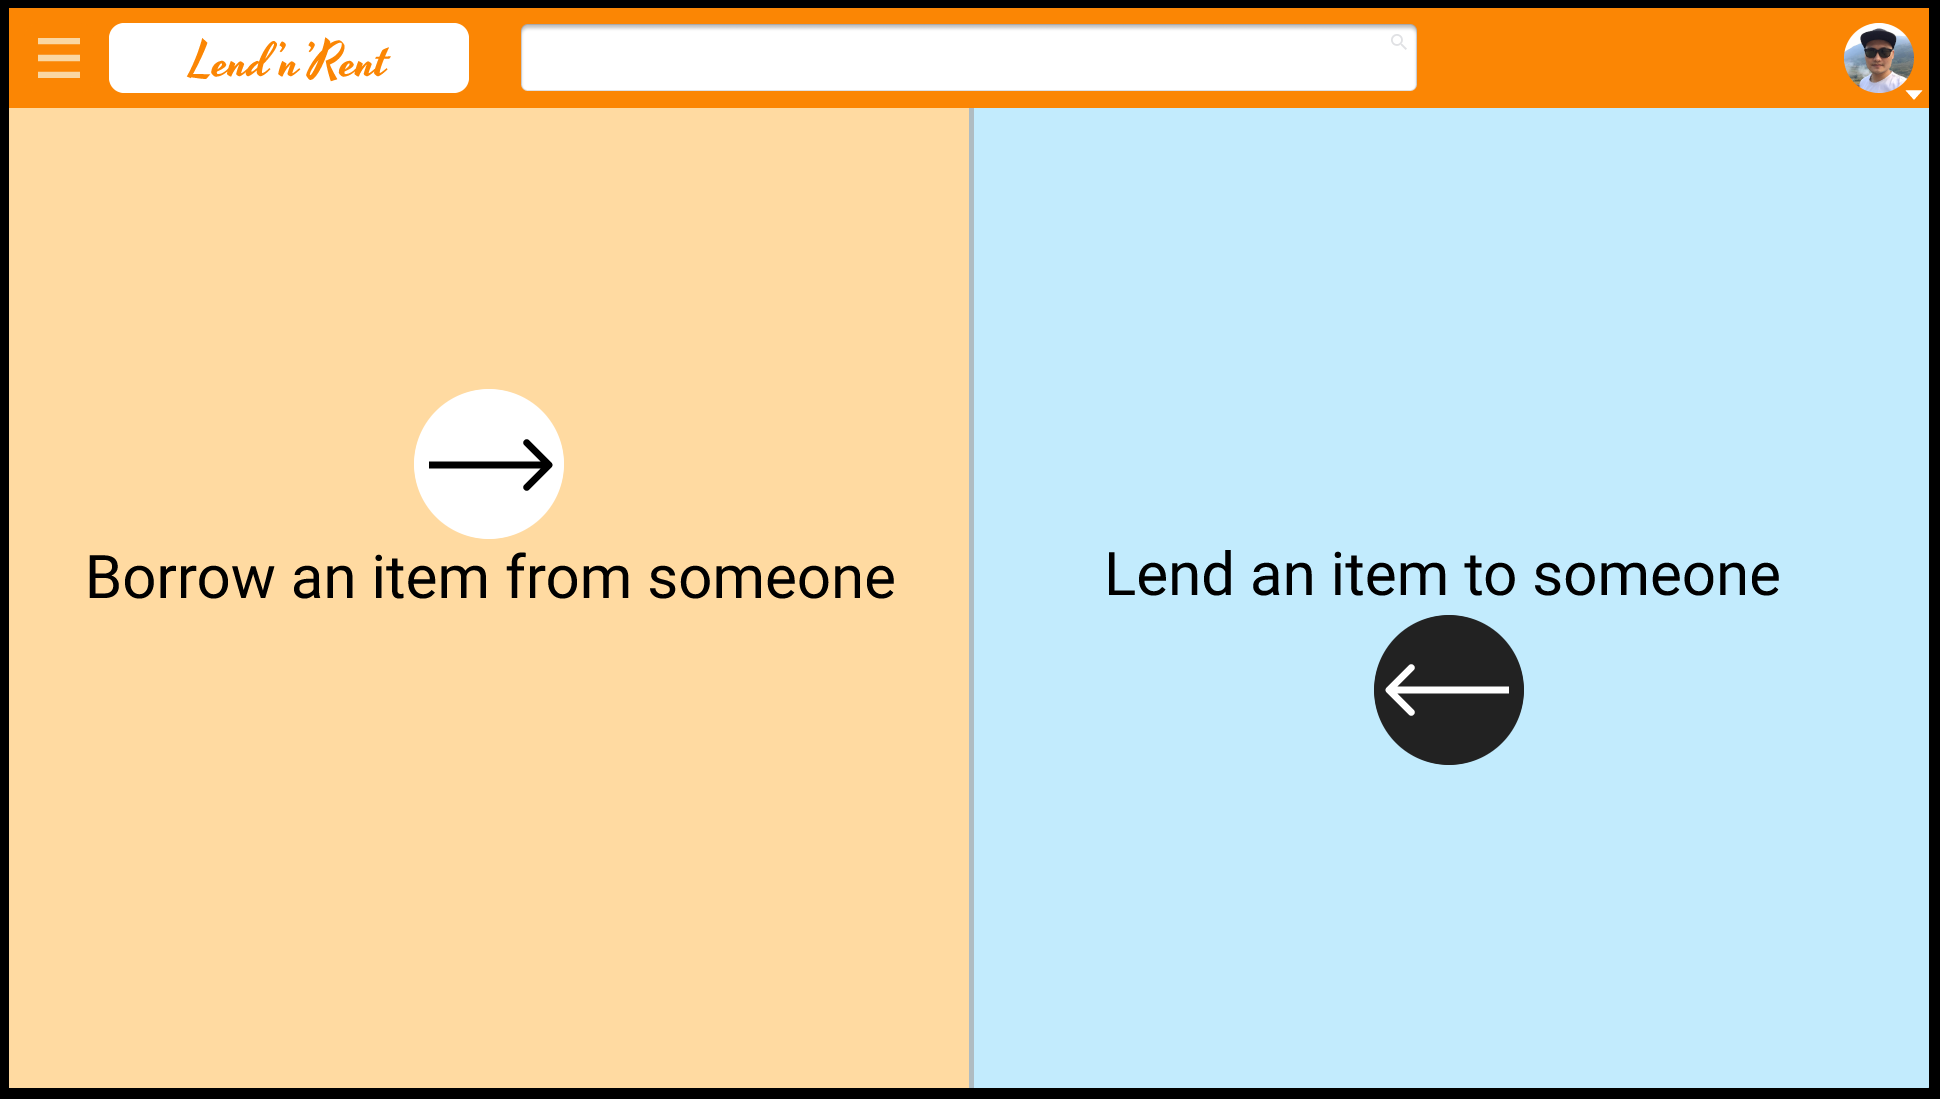
\includegraphics[width=0.5\linewidth]{abb/1landing}
	\caption{Landing page}
	\label{fig:1landing}
\end{figure} 

\noindent
The unique color design of our website makes it always obvious to the user whether he is in the role of lender or renter. If the user rents items, his profile page will also be displayed in the respective blue color scheme, or in orange if he removes all items.

\begin{figure}[H]
	\centering
	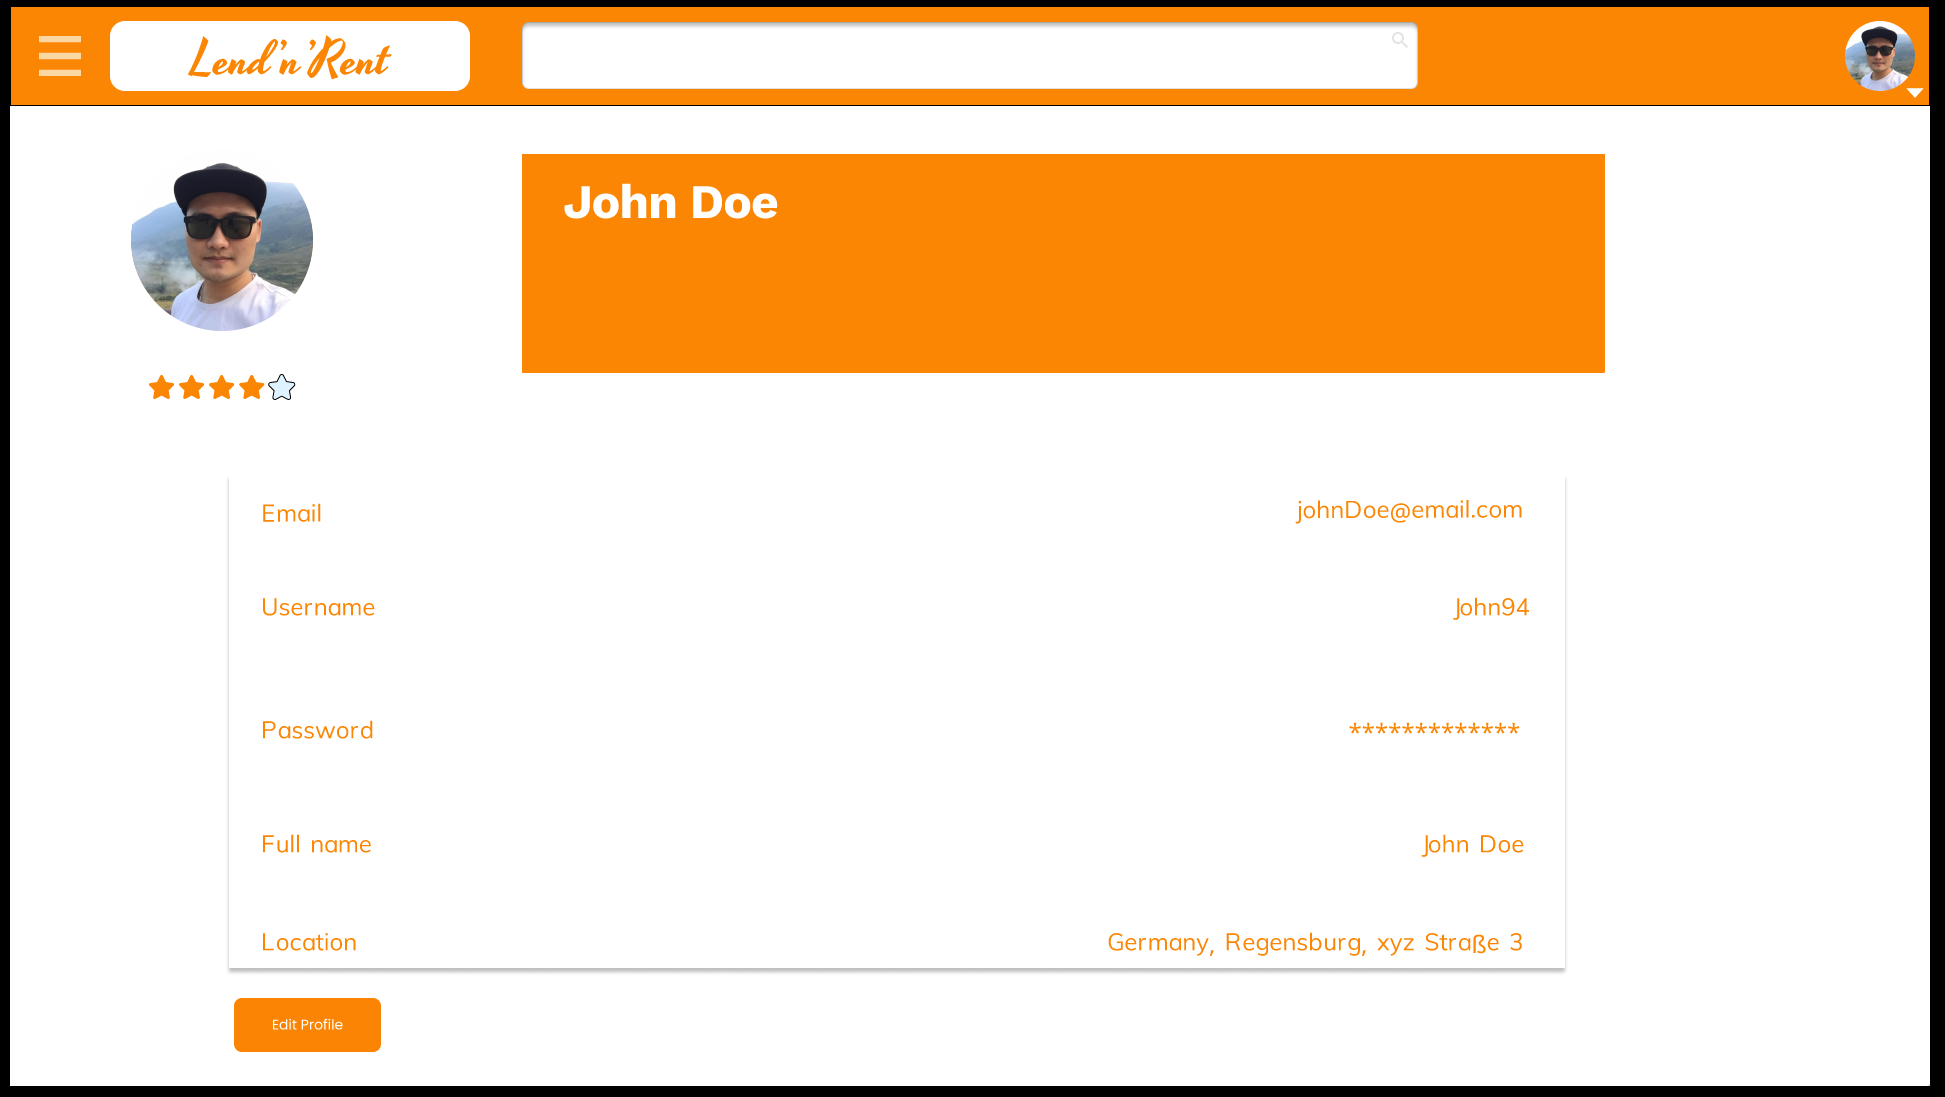
\includegraphics[width=0.49\linewidth]{abb/11profilerent}
	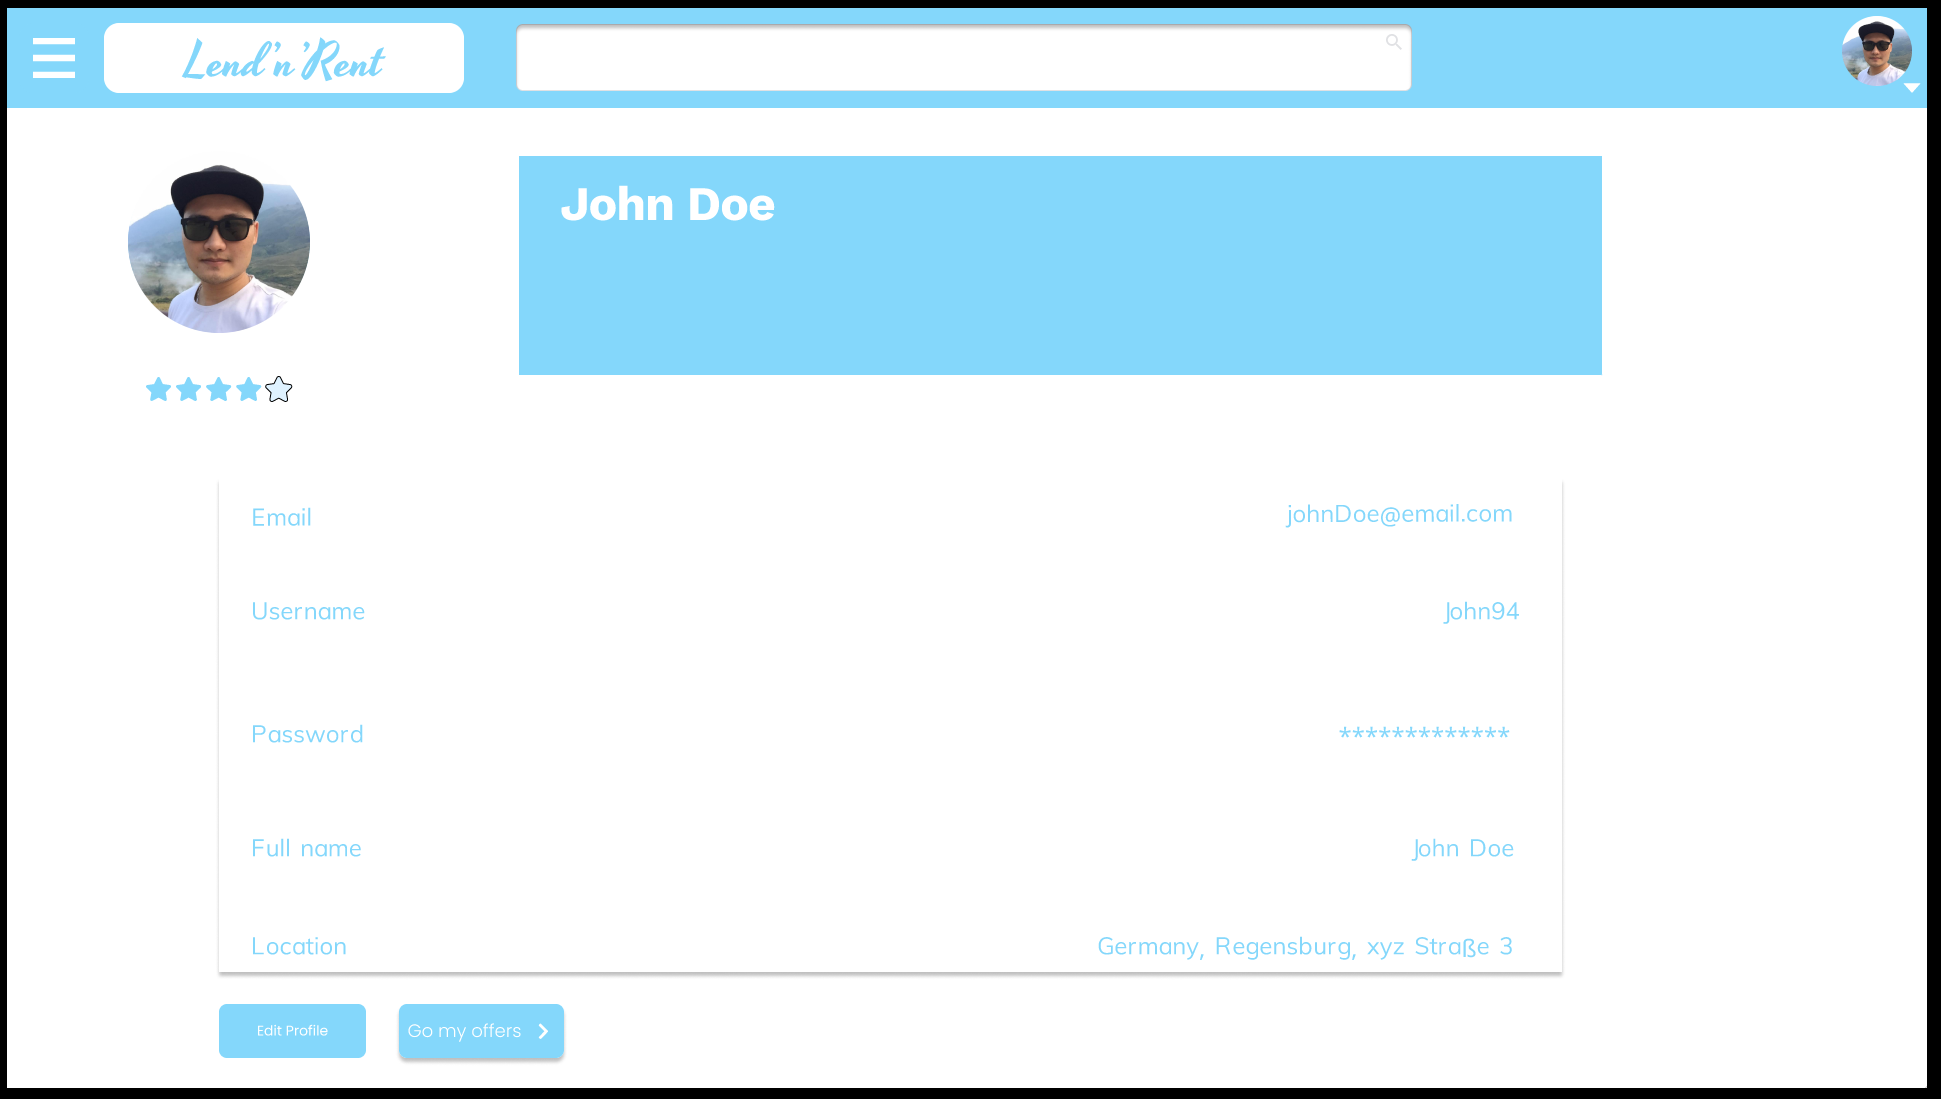
\includegraphics[width=0.49\linewidth]{abb/6profilelend}
	\caption{Profilepage lender and renter}
	\label{fig:profile}
	\centering
\end{figure}

\noindent
The create an offer process is very simple and allows the lender to compare his item with others in order to choose a competitive price.

\begin{figure}[H]
	\centering
	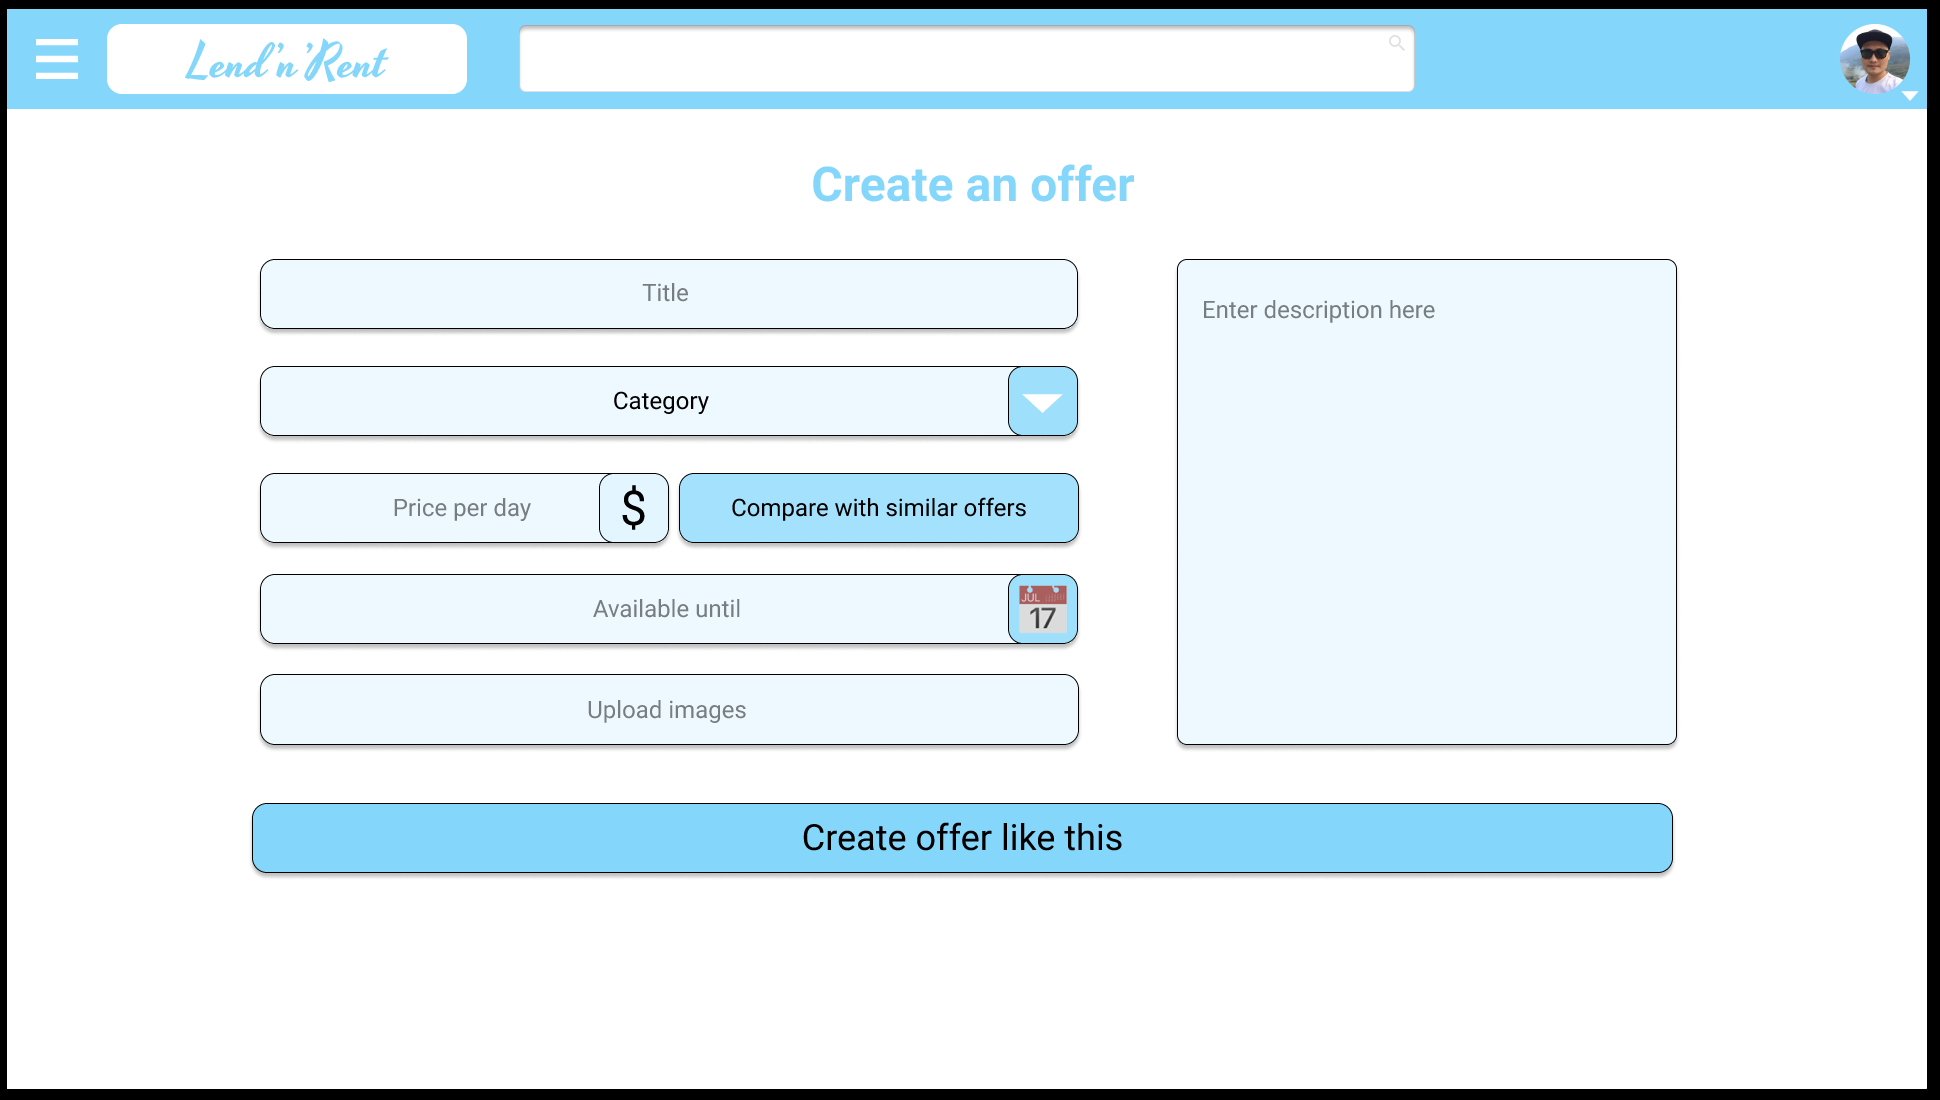
\includegraphics[width=0.5\linewidth]{abb/2offer}
	\caption{Create offer}
	\label{fig:2offer}
\end{figure} 

\noindent
After creating the offer, the user is navigated to the item page to get an overview and make any changes. An overview of all items can be found on the my offers page.

\begin{figure}[H]
	\centering
	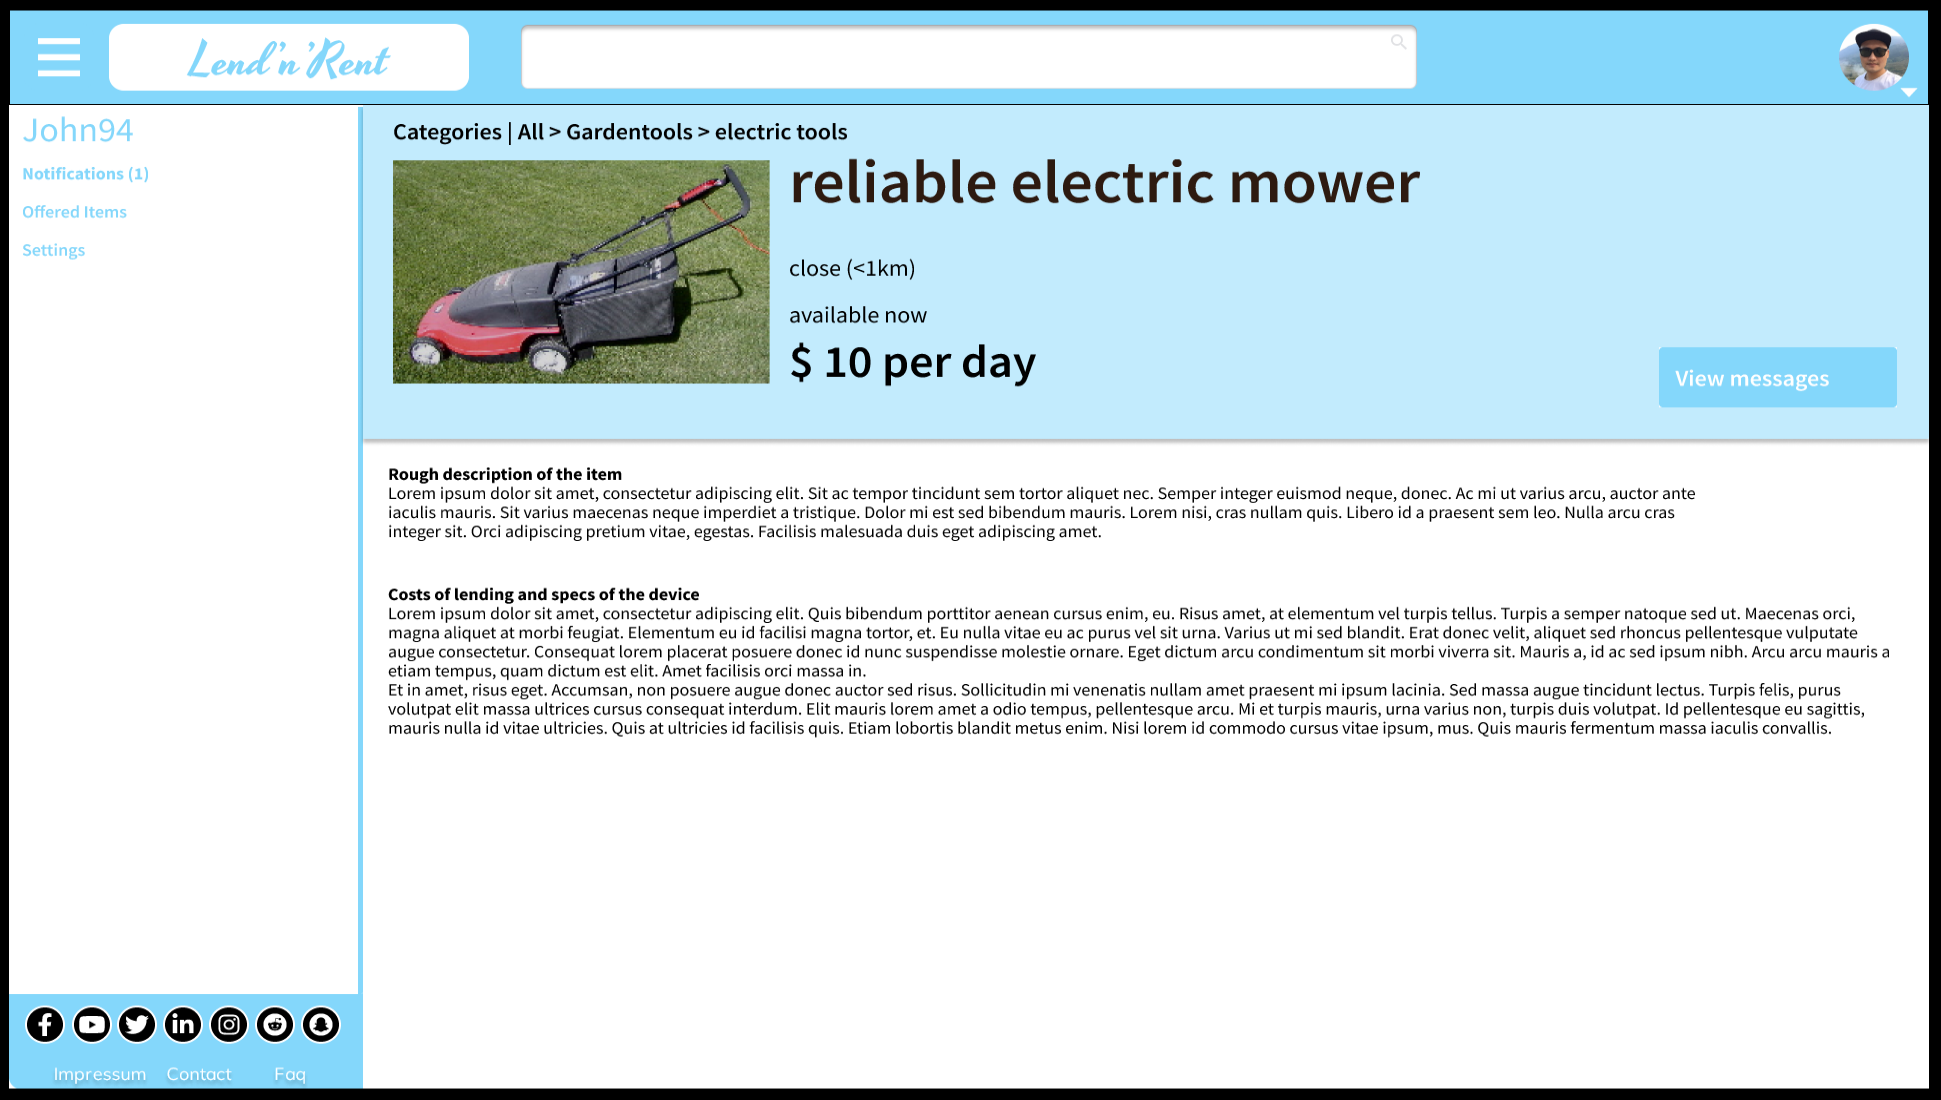
\includegraphics[width=0.49\linewidth]{abb/4item}
	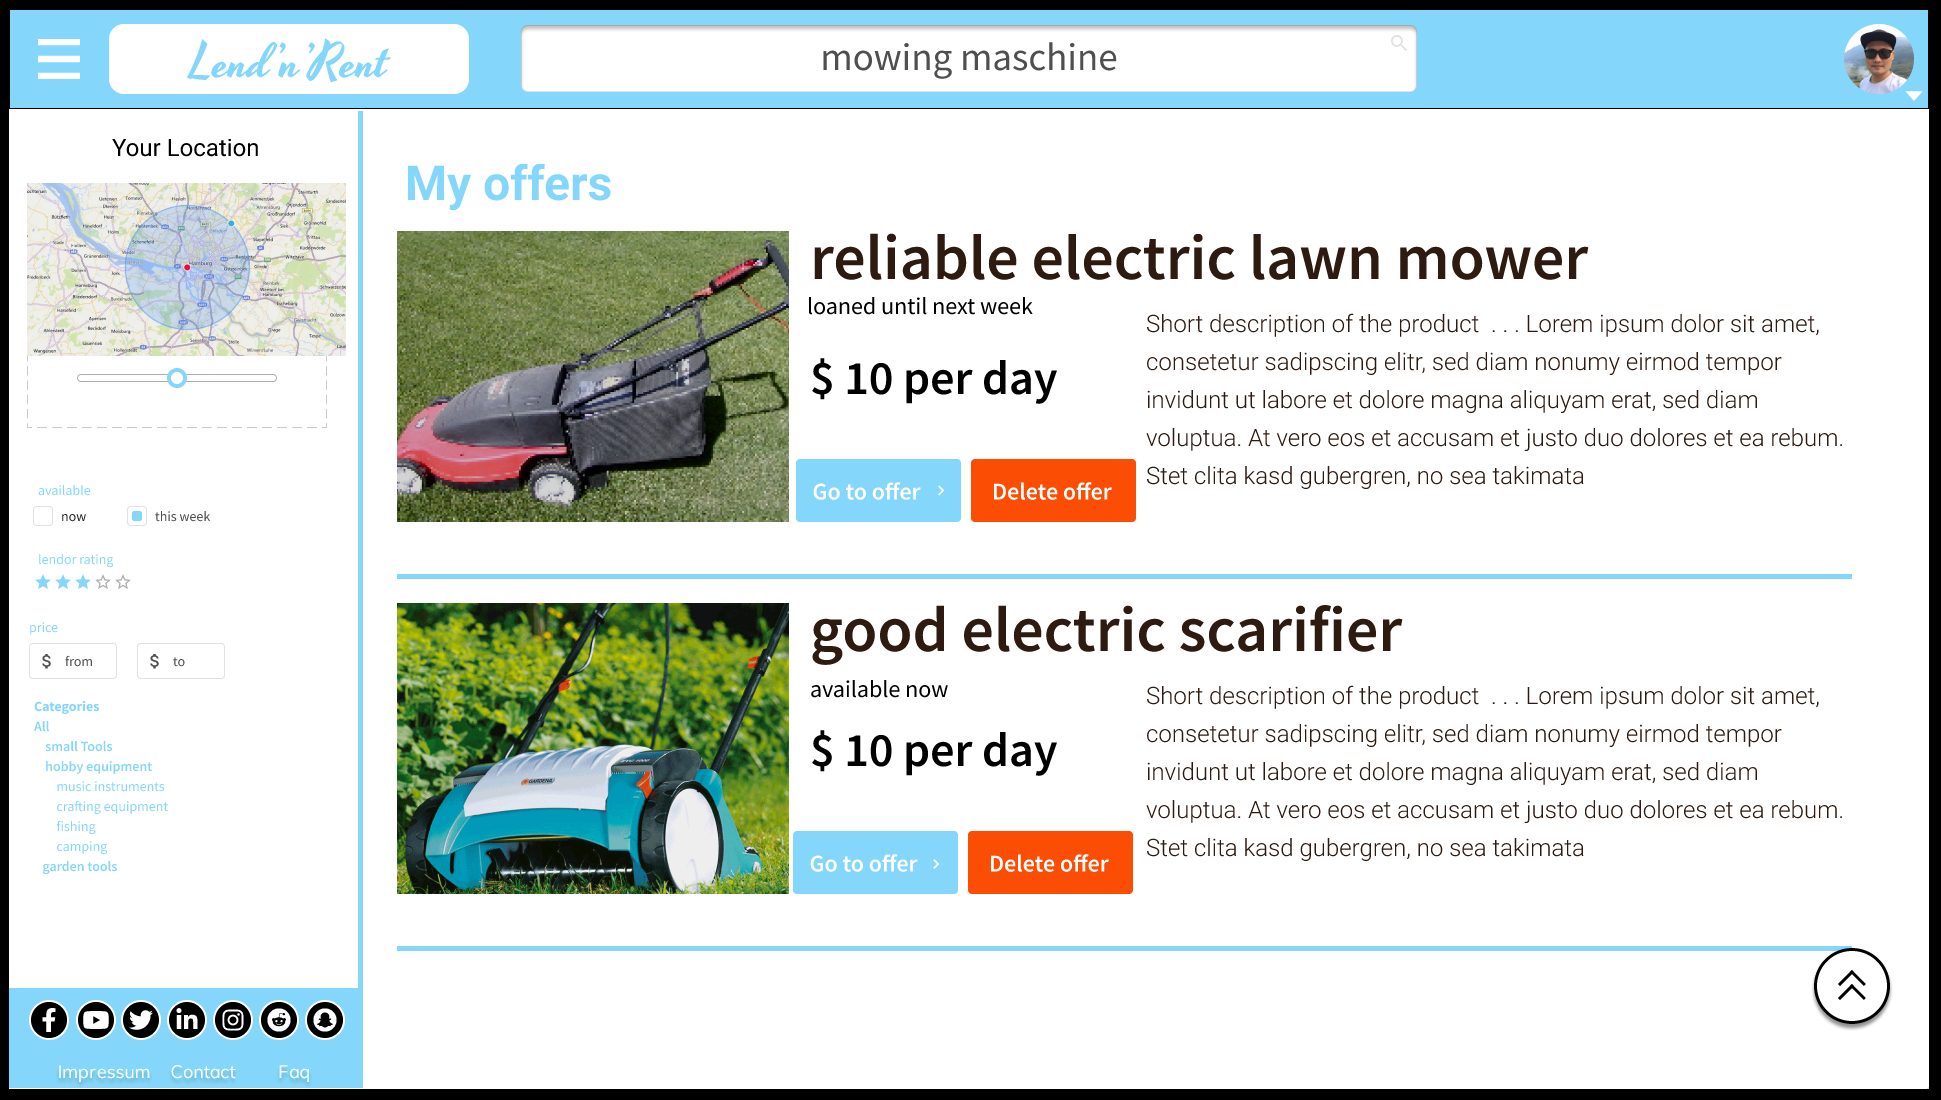
\includegraphics[width=0.49\linewidth]{abb/3offers}
	\caption{Article and offers page}
	\label{fig:article}
	\centering
\end{figure}

\noindent
The category page is designed so that the individual categories are displayed as large images. The idea behind this is not to flood the user with a lot of information, but to leave it up to the user to make a concrete decision.

\begin{figure}[H]
	\centering
	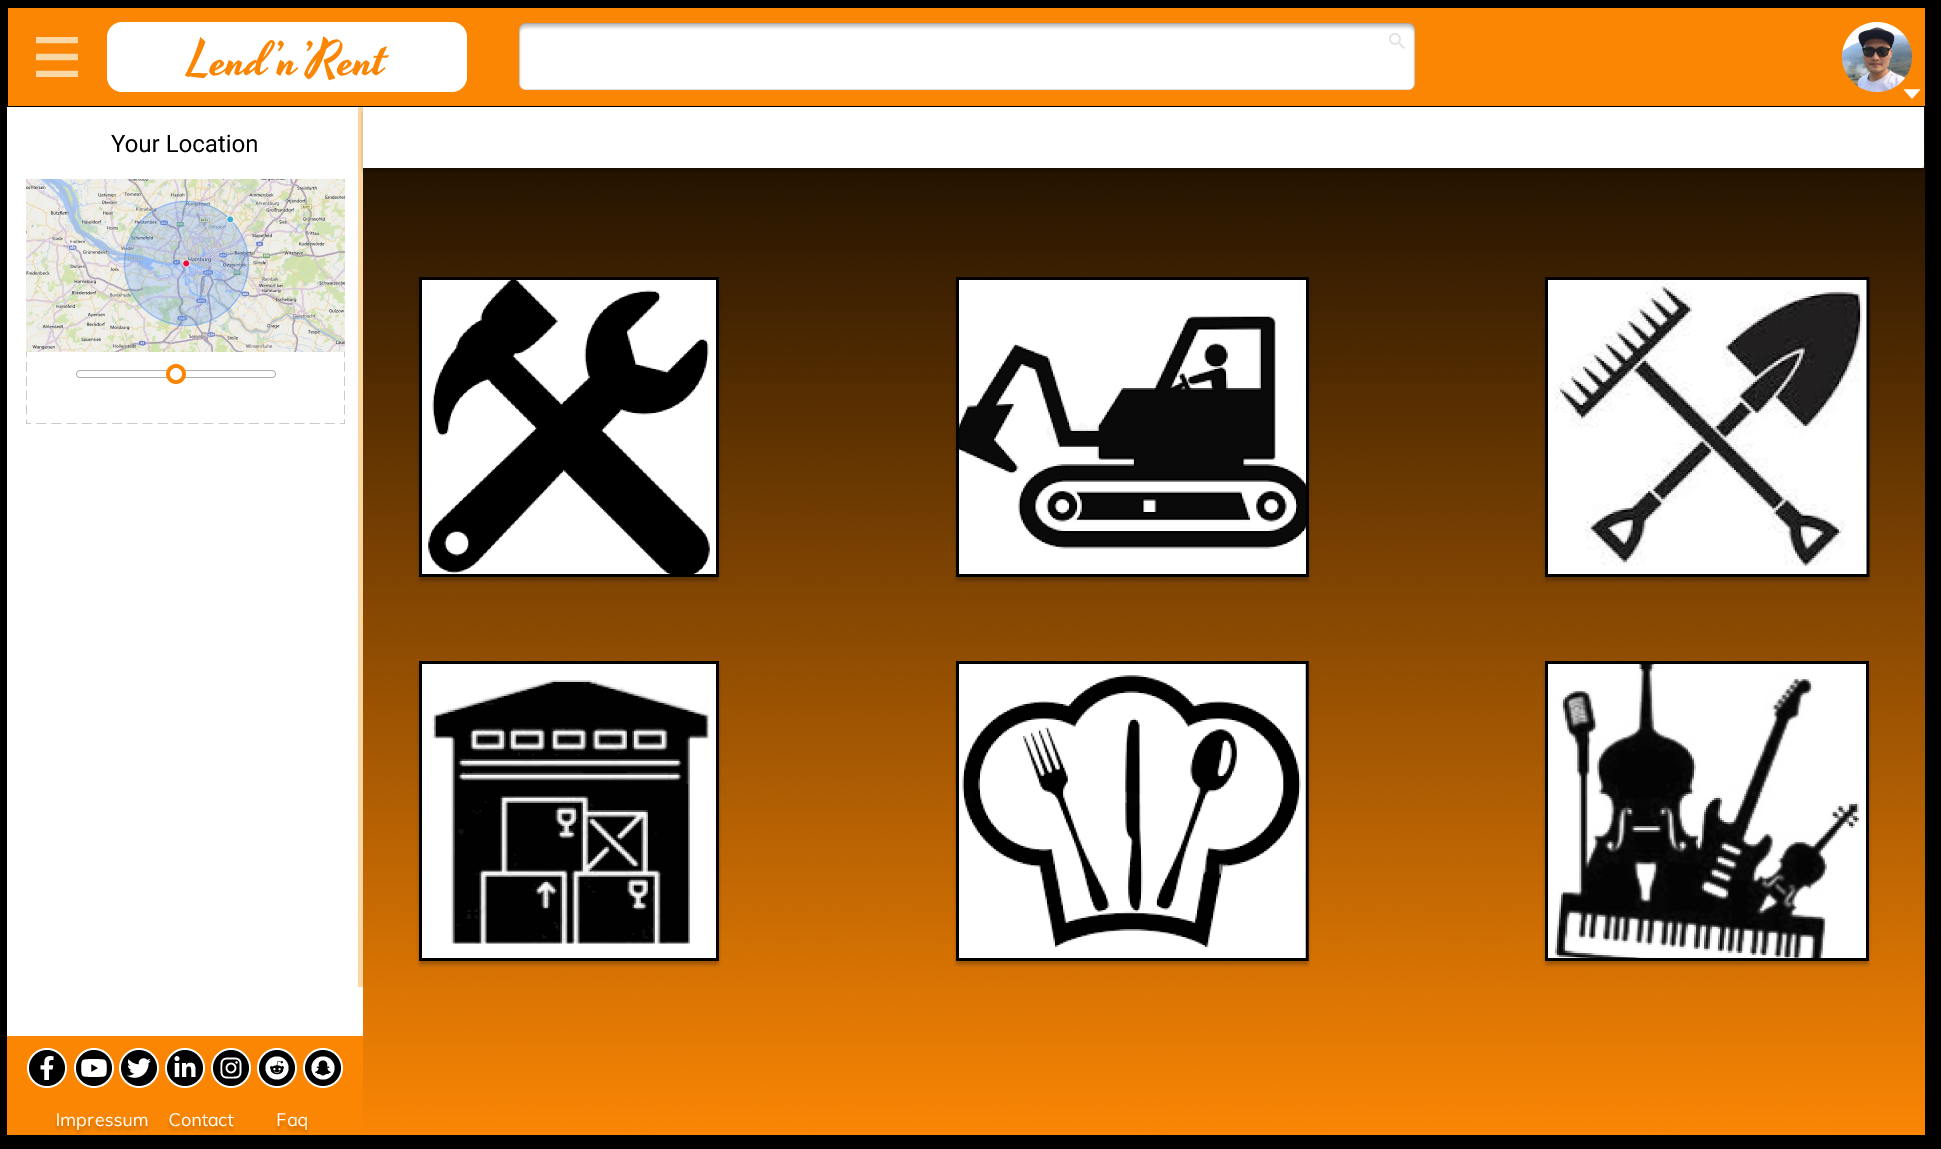
\includegraphics[width=0.5\linewidth]{abb/8start}
	\caption{Category page}
	\label{fig:8start}
\end{figure} 

\noindent
Only after the user has chosen a category, he will be redirected to the search page and the items from this category will be displayed.
On the search page the user has the possibility to choose a subcategory, set the search radius, price range, availability and average rating.

\begin{figure}[H]
	\centering
	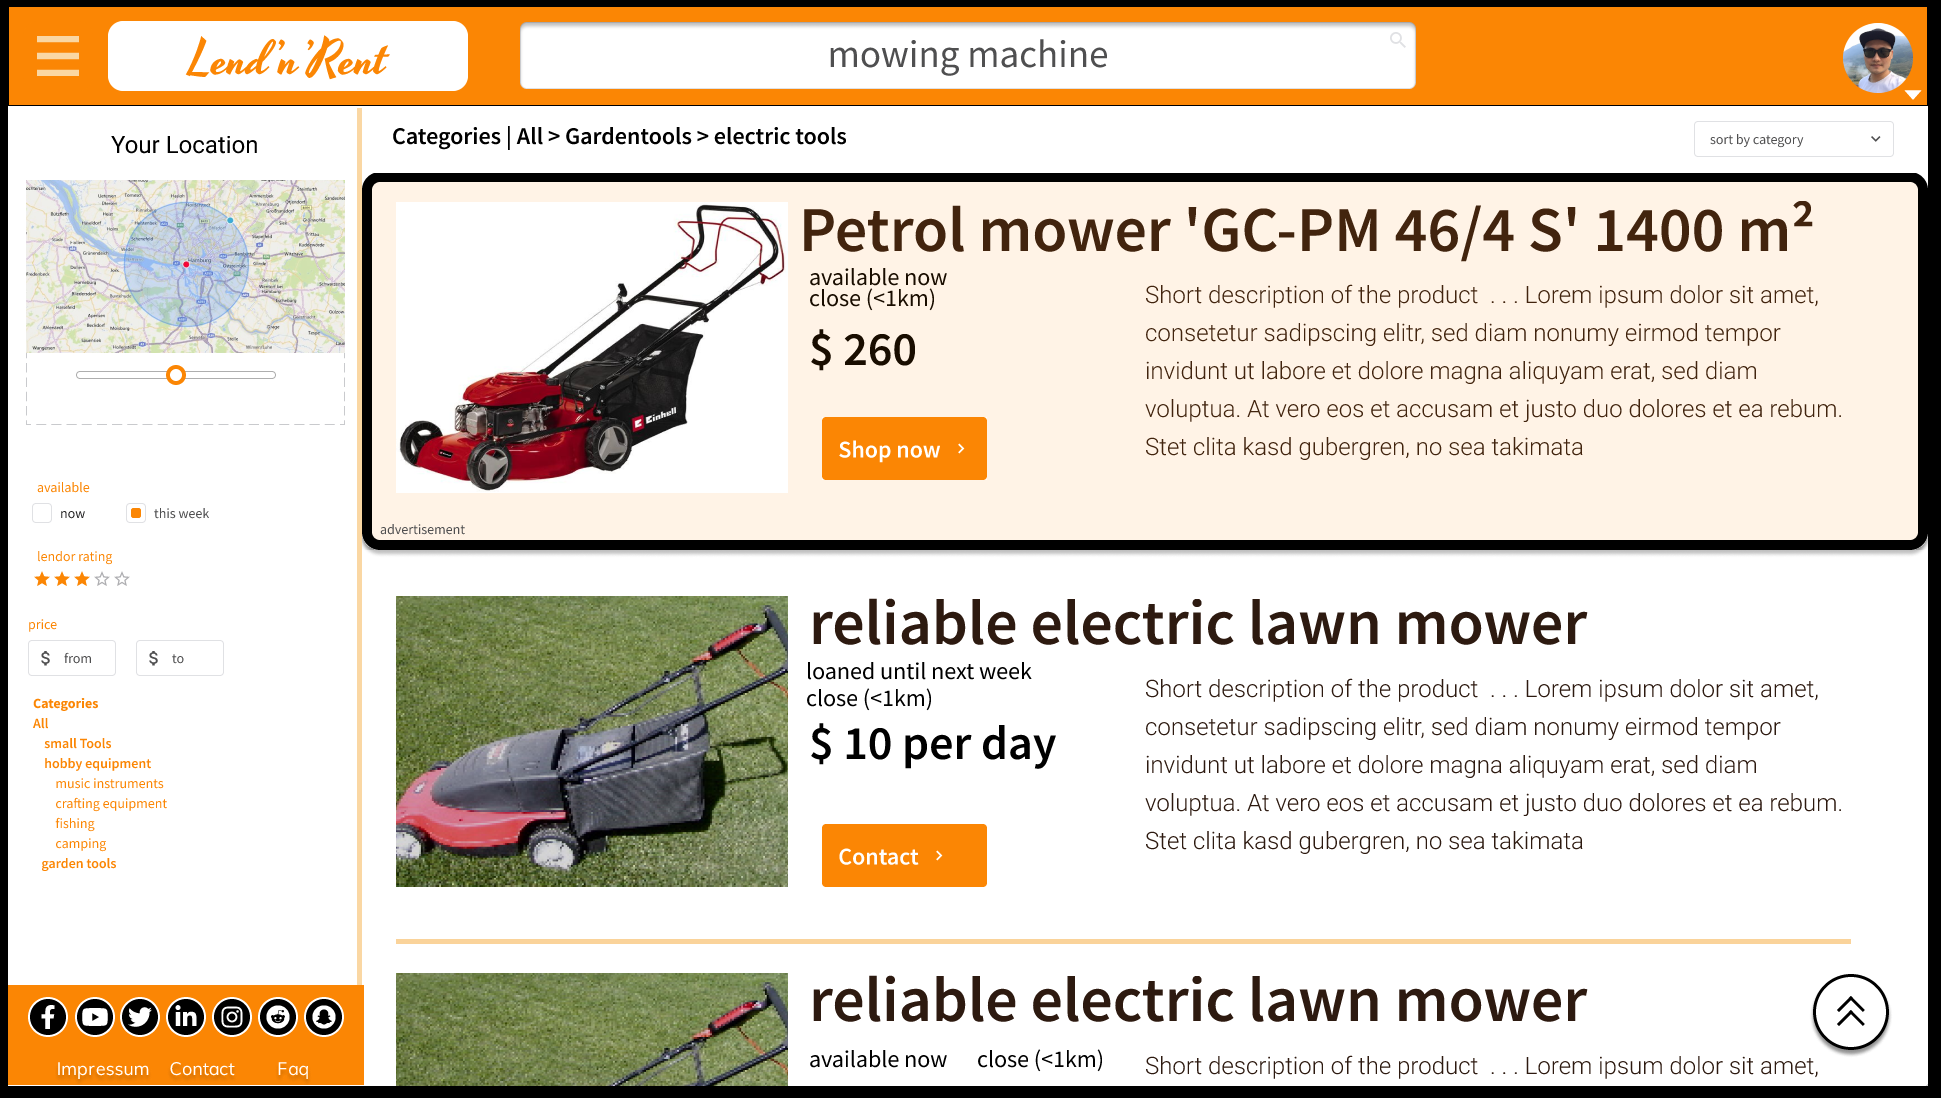
\includegraphics[width=0.49\linewidth]{abb/9search}
	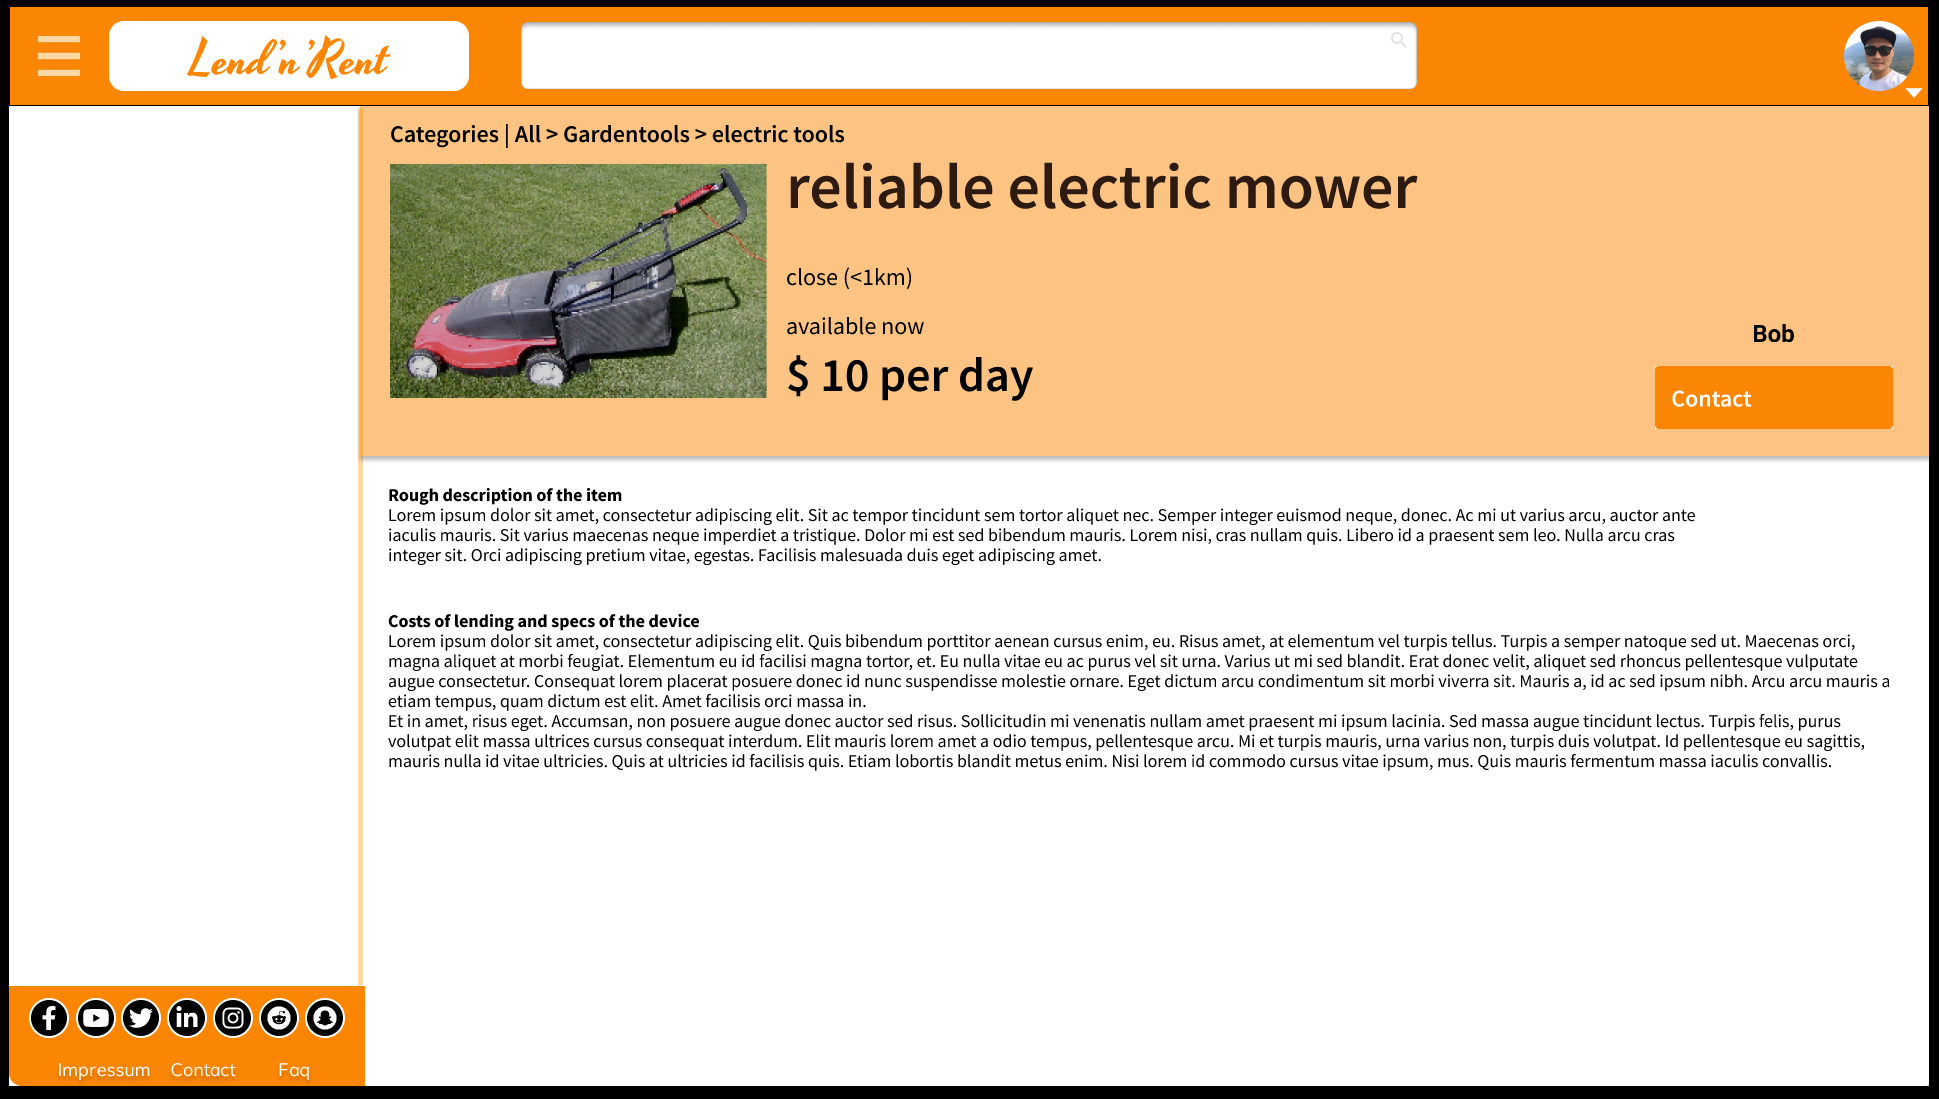
\includegraphics[width=0.49\linewidth]{abb/10itemrent}
	\caption{Search and article page renter role}
	\label{fig:search}
	\centering
\end{figure}

\newpage
\noindent
As soon as the user has chosen an item, he has the possibility to contact the lender via the article page.

\begin{figure}[H]
	\centering
	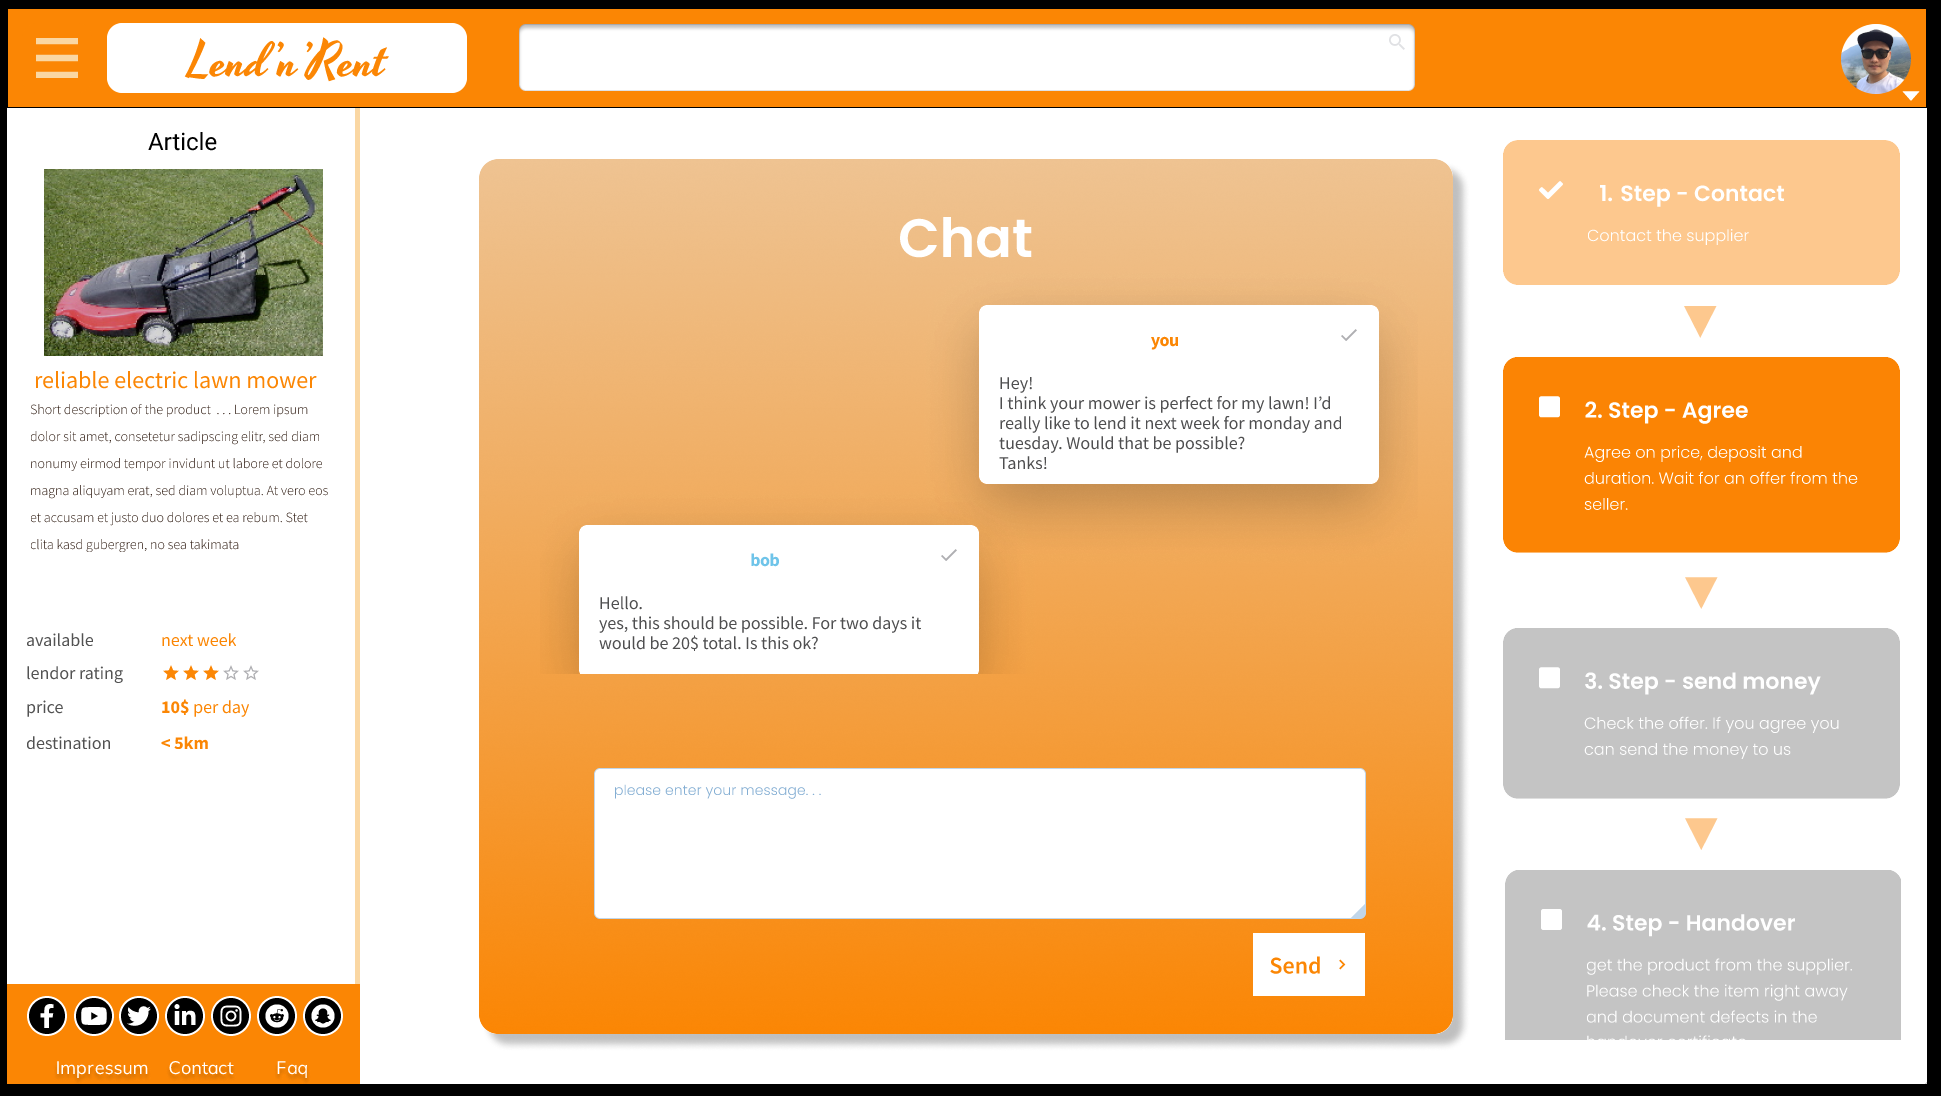
\includegraphics[width=0.49\linewidth]{abb/12step2}
	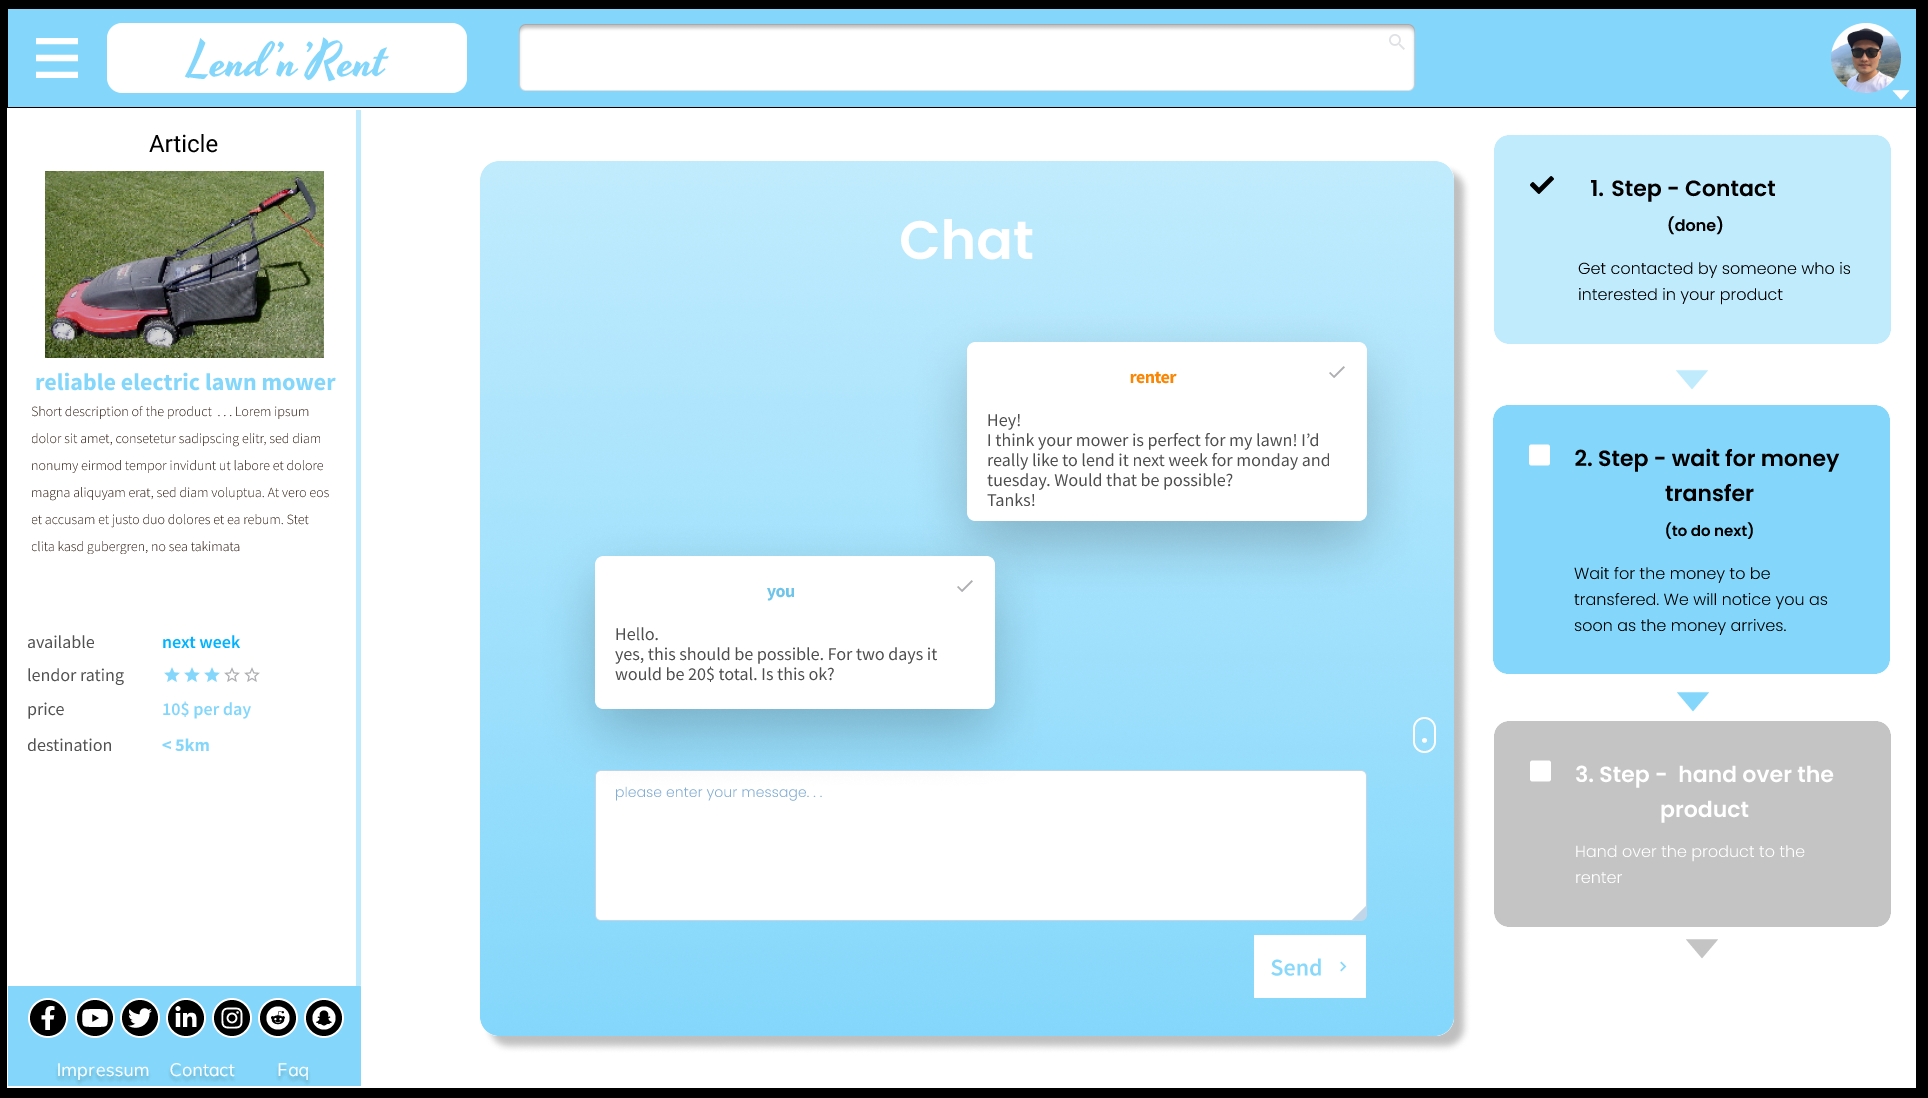
\includegraphics[width=0.49\linewidth]{abb/5step1}
	\caption{Negotiation Step 1 Contact and Agreement}
	\label{fig:negotiation1}
	\centering
\end{figure}

\noindent
Once the users have agreed, the renter must fill in and confirm the offer form.

\begin{figure}[H]
	\centering
	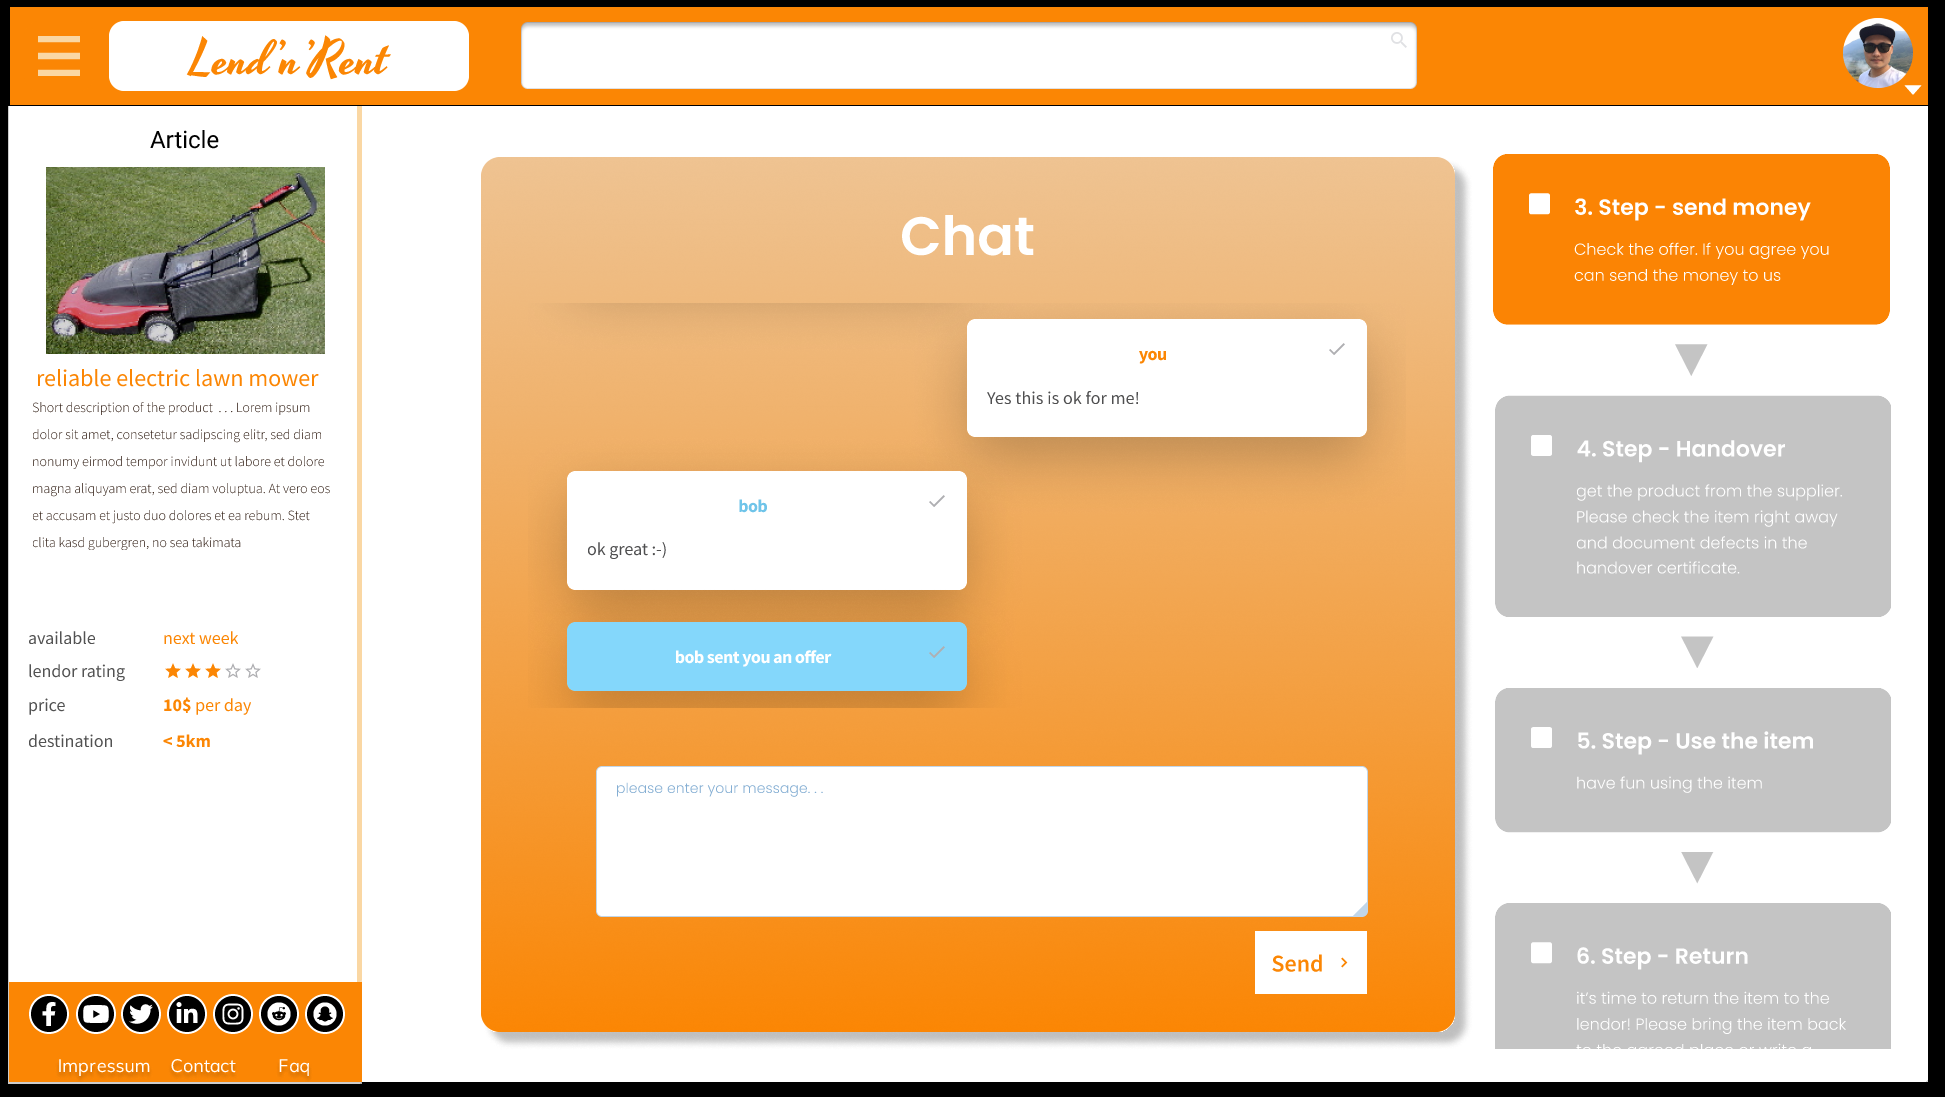
\includegraphics[width=0.49\linewidth]{abb/13step3}
	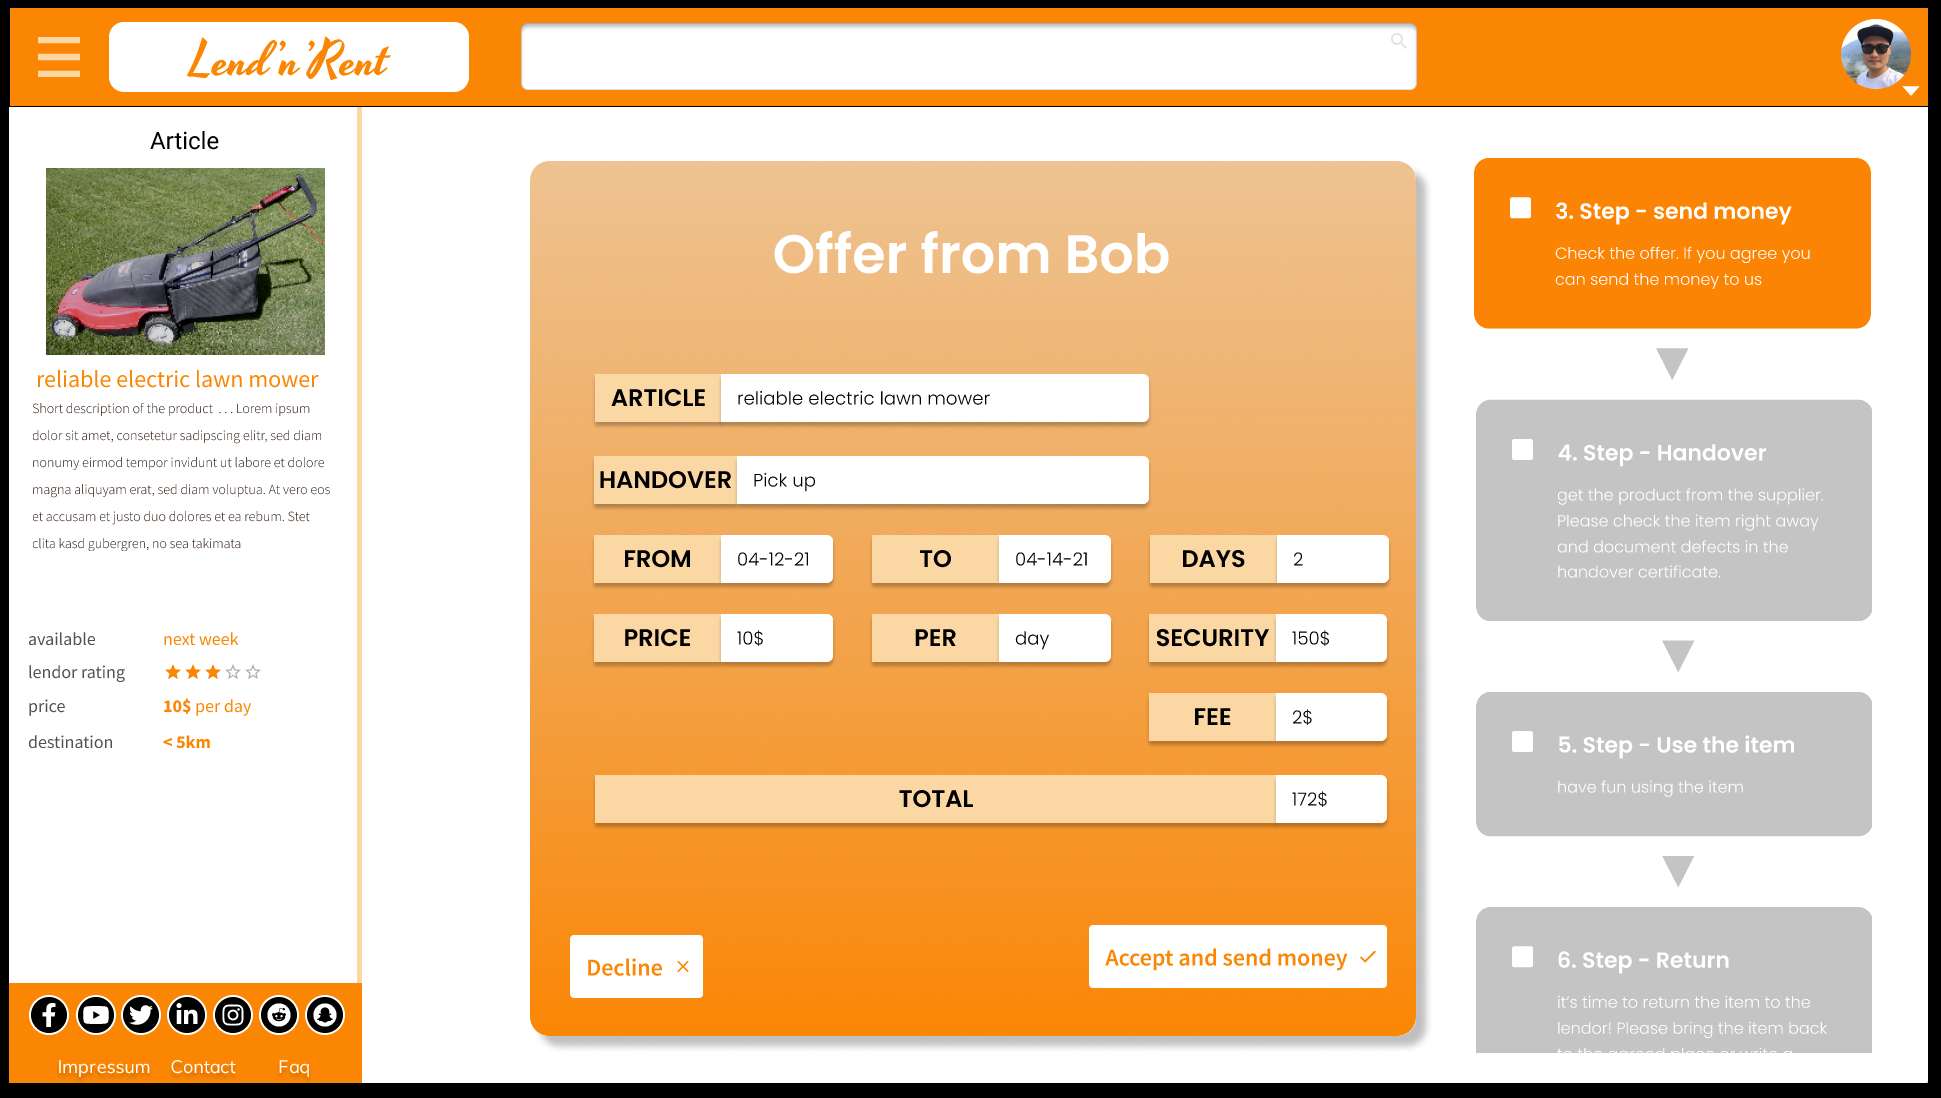
\includegraphics[width=0.49\linewidth]{abb/14step3con}
	\caption{Negotiation Step 3 Payment agreements}
	\label{fig:Negotiation2}
	\centering
\end{figure}

\noindent
After the handover, the renter must inspect the item and describe its condition in the "Handover Certificate" and send the certificate.

\begin{figure}[H]
	\centering
	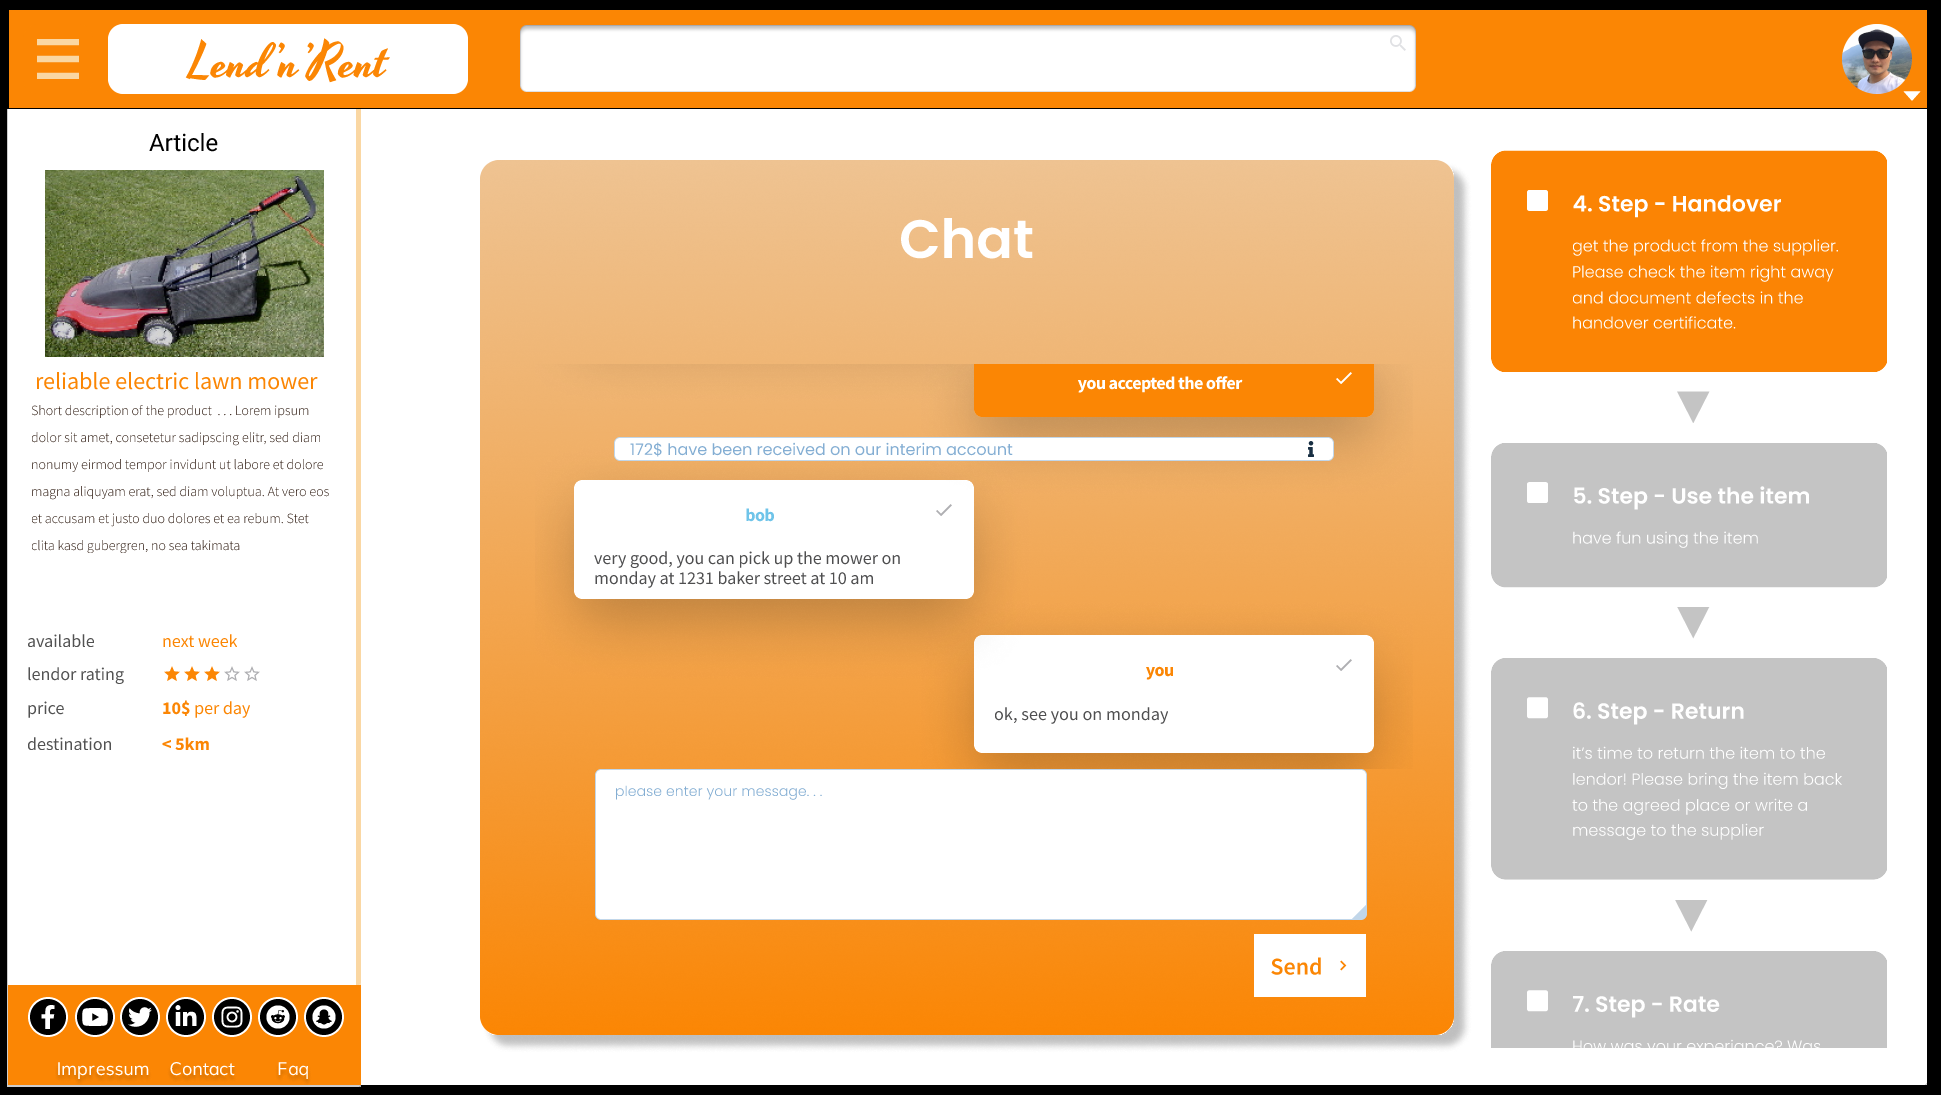
\includegraphics[width=0.49\linewidth]{abb/15step4}
	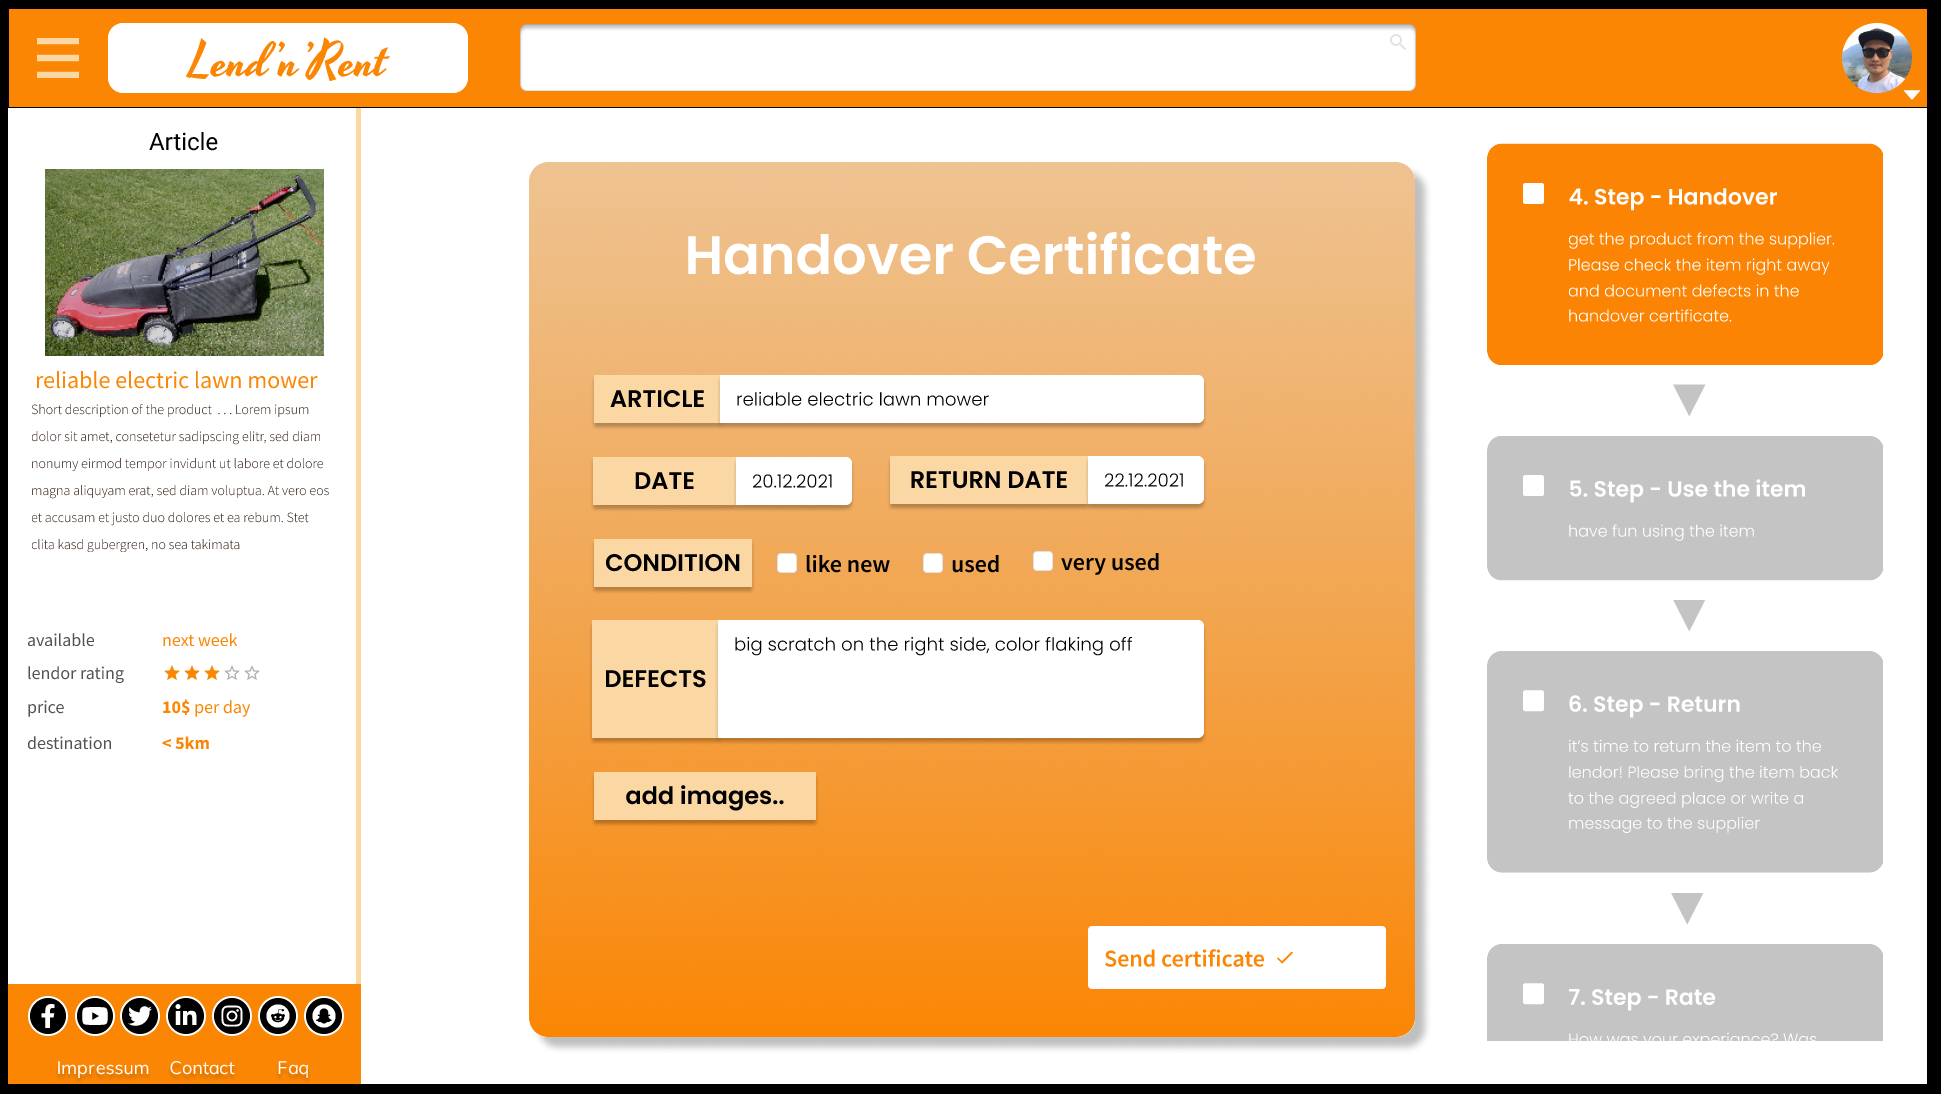
\includegraphics[width=0.49\linewidth]{abb/16step4con}
	\caption{Negotiation Step 4 Handover Certificate}
	\label{fig:Negotiation3}
	\centering
\end{figure}

\newpage
\noindent
After the transfer of the certificate, the renter can use the item. About the time of return both will be notified in time and have the opportunity to clarify the exact time in the chat.

\begin{figure}[H]
	\centering
	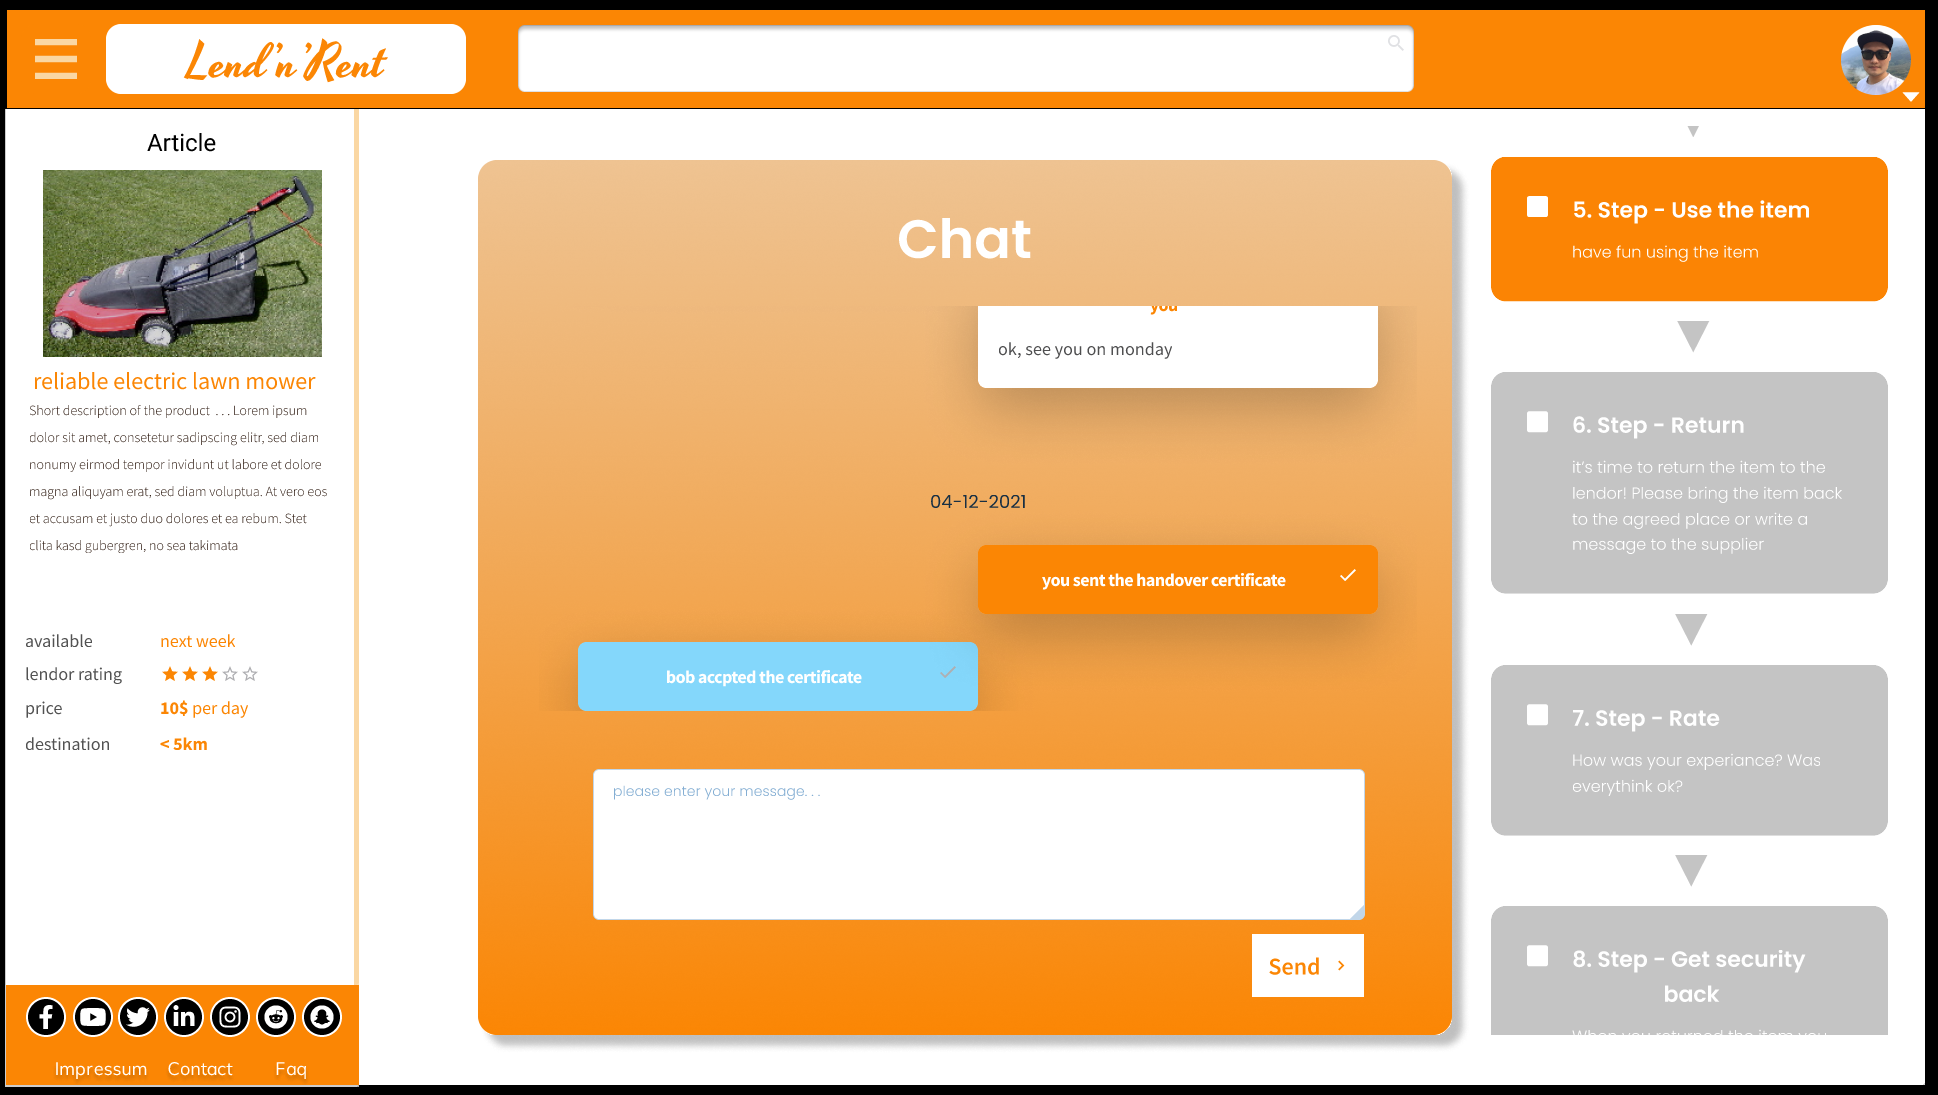
\includegraphics[width=0.49\linewidth]{abb/17step5}
	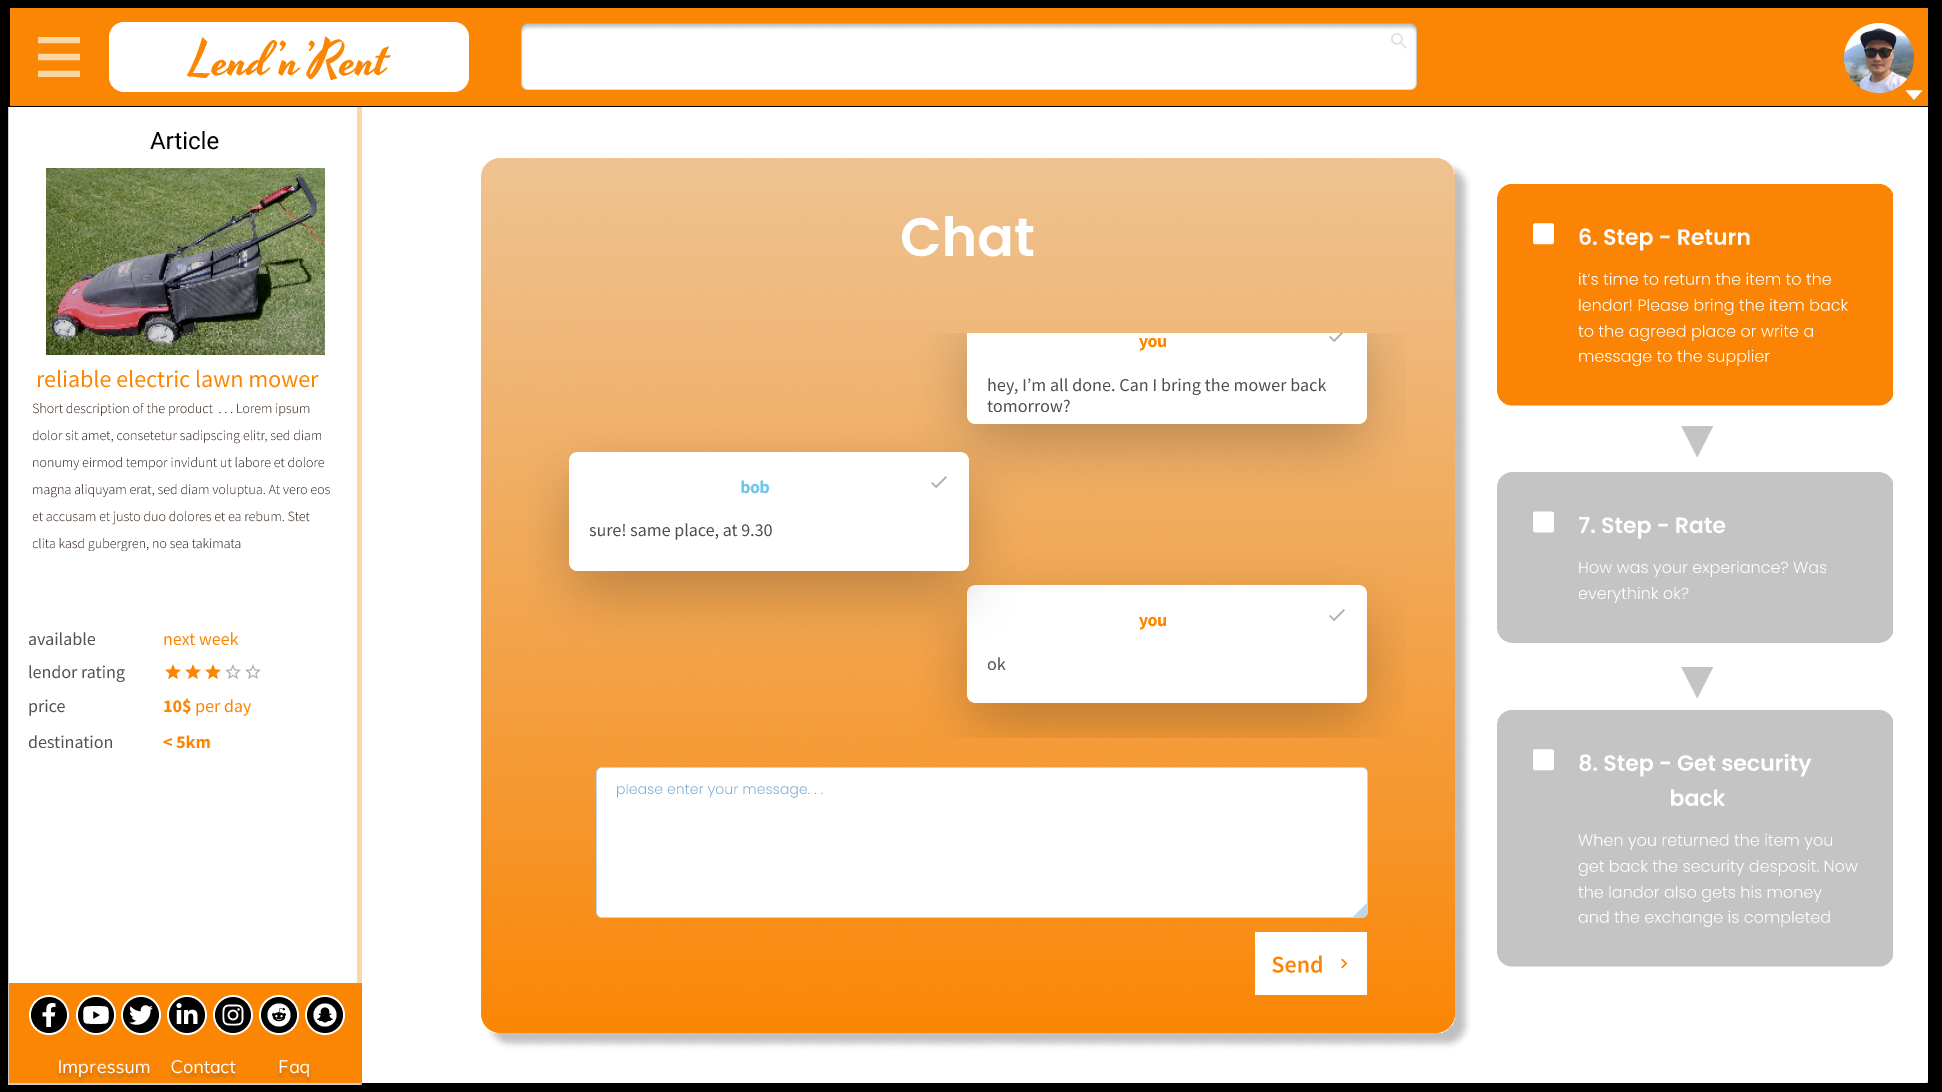
\includegraphics[width=0.49\linewidth]{abb/18step6}
	\caption{Use and Return}
	\label{fig:Negotiation4}
	\centering
\end{figure}

\noindent
After the return, the renter can rate the lender. if the item is returned in the same working condition, the renter gets back his security deposit and the lender gets the money.

\begin{figure}[H]
	\centering
	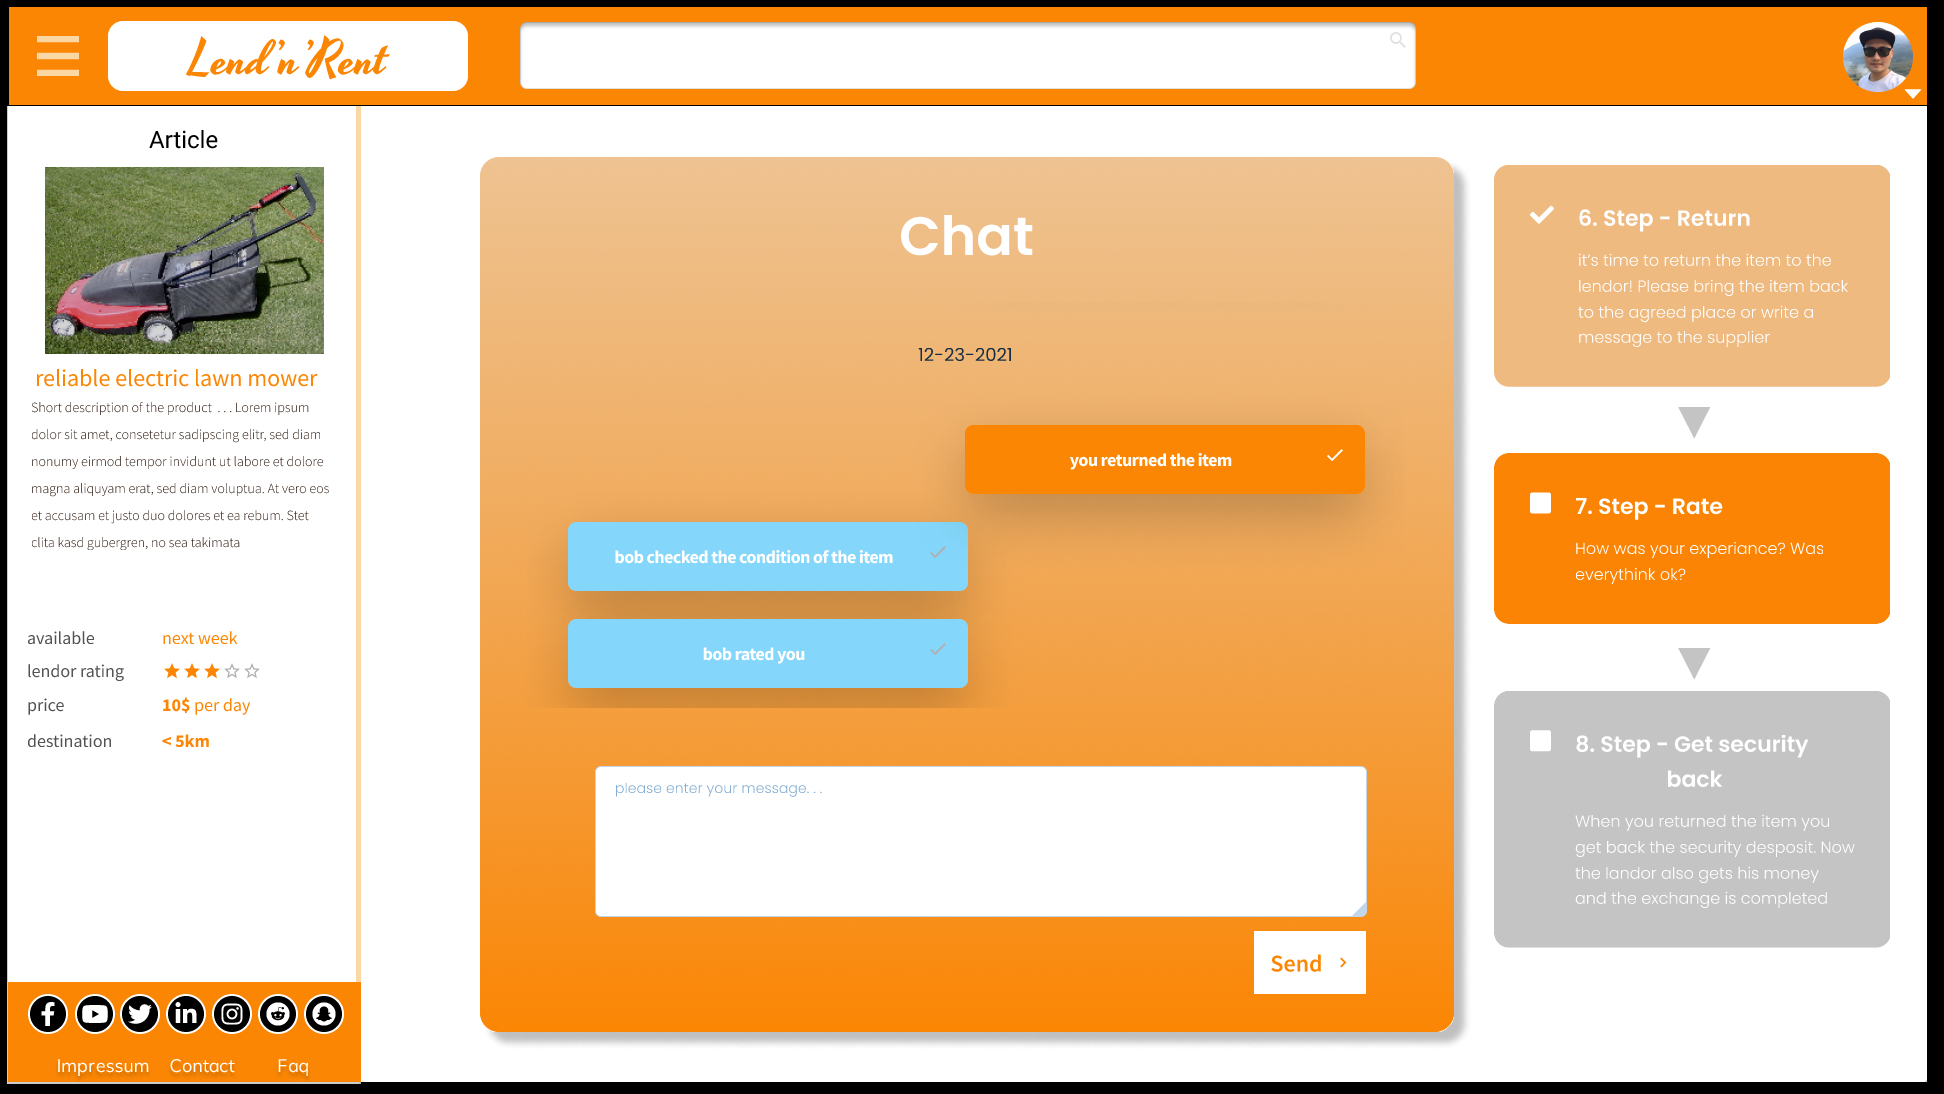
\includegraphics[width=0.49\linewidth]{abb/19step7}
	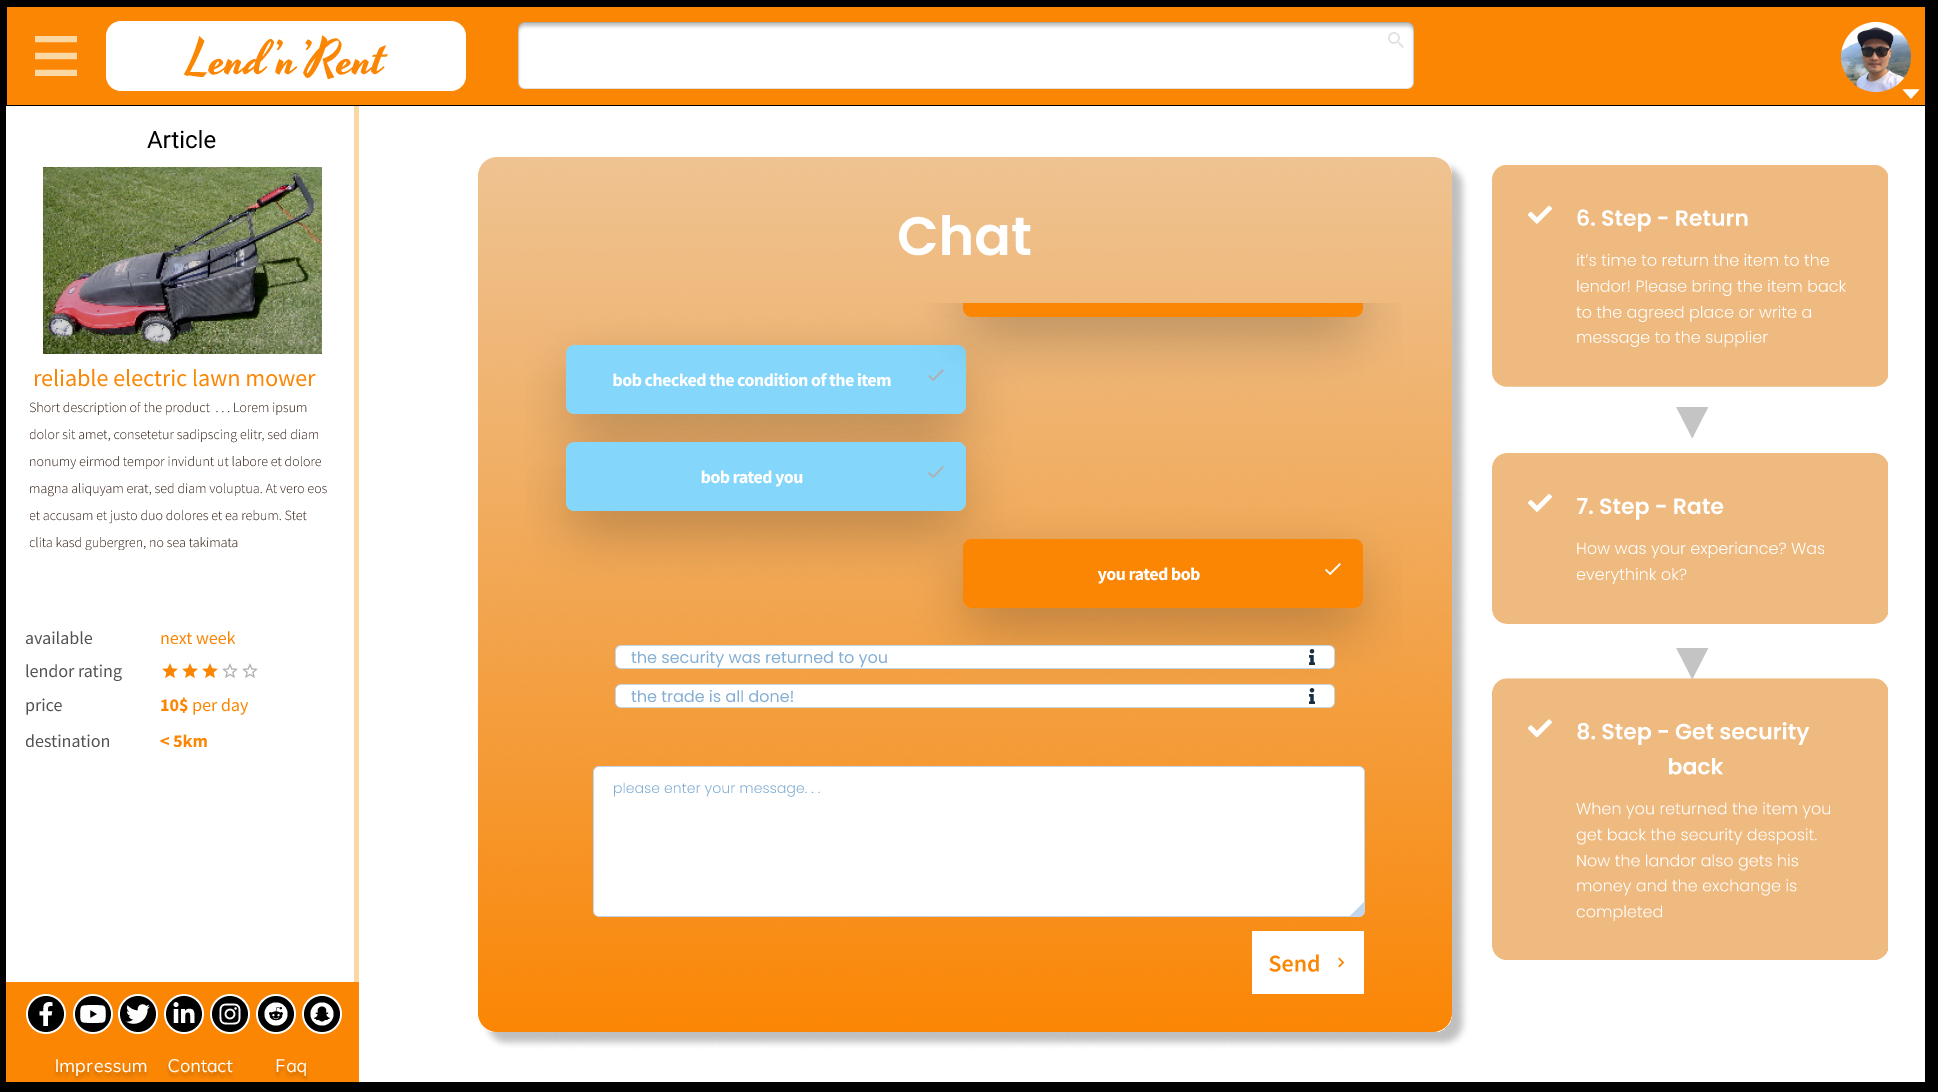
\includegraphics[width=0.49\linewidth]{abb/20steplast}
	\caption{Rating and Payment}
	\label{fig:Negotiation5}
	\centering
\end{figure}

\noindent
The design of the message page is adapted to the page design. In this way, the user can always distinguish whether he is accessing the messages with requests or those where he wants to rent something himself.

\begin{figure}[H]
	\centering
	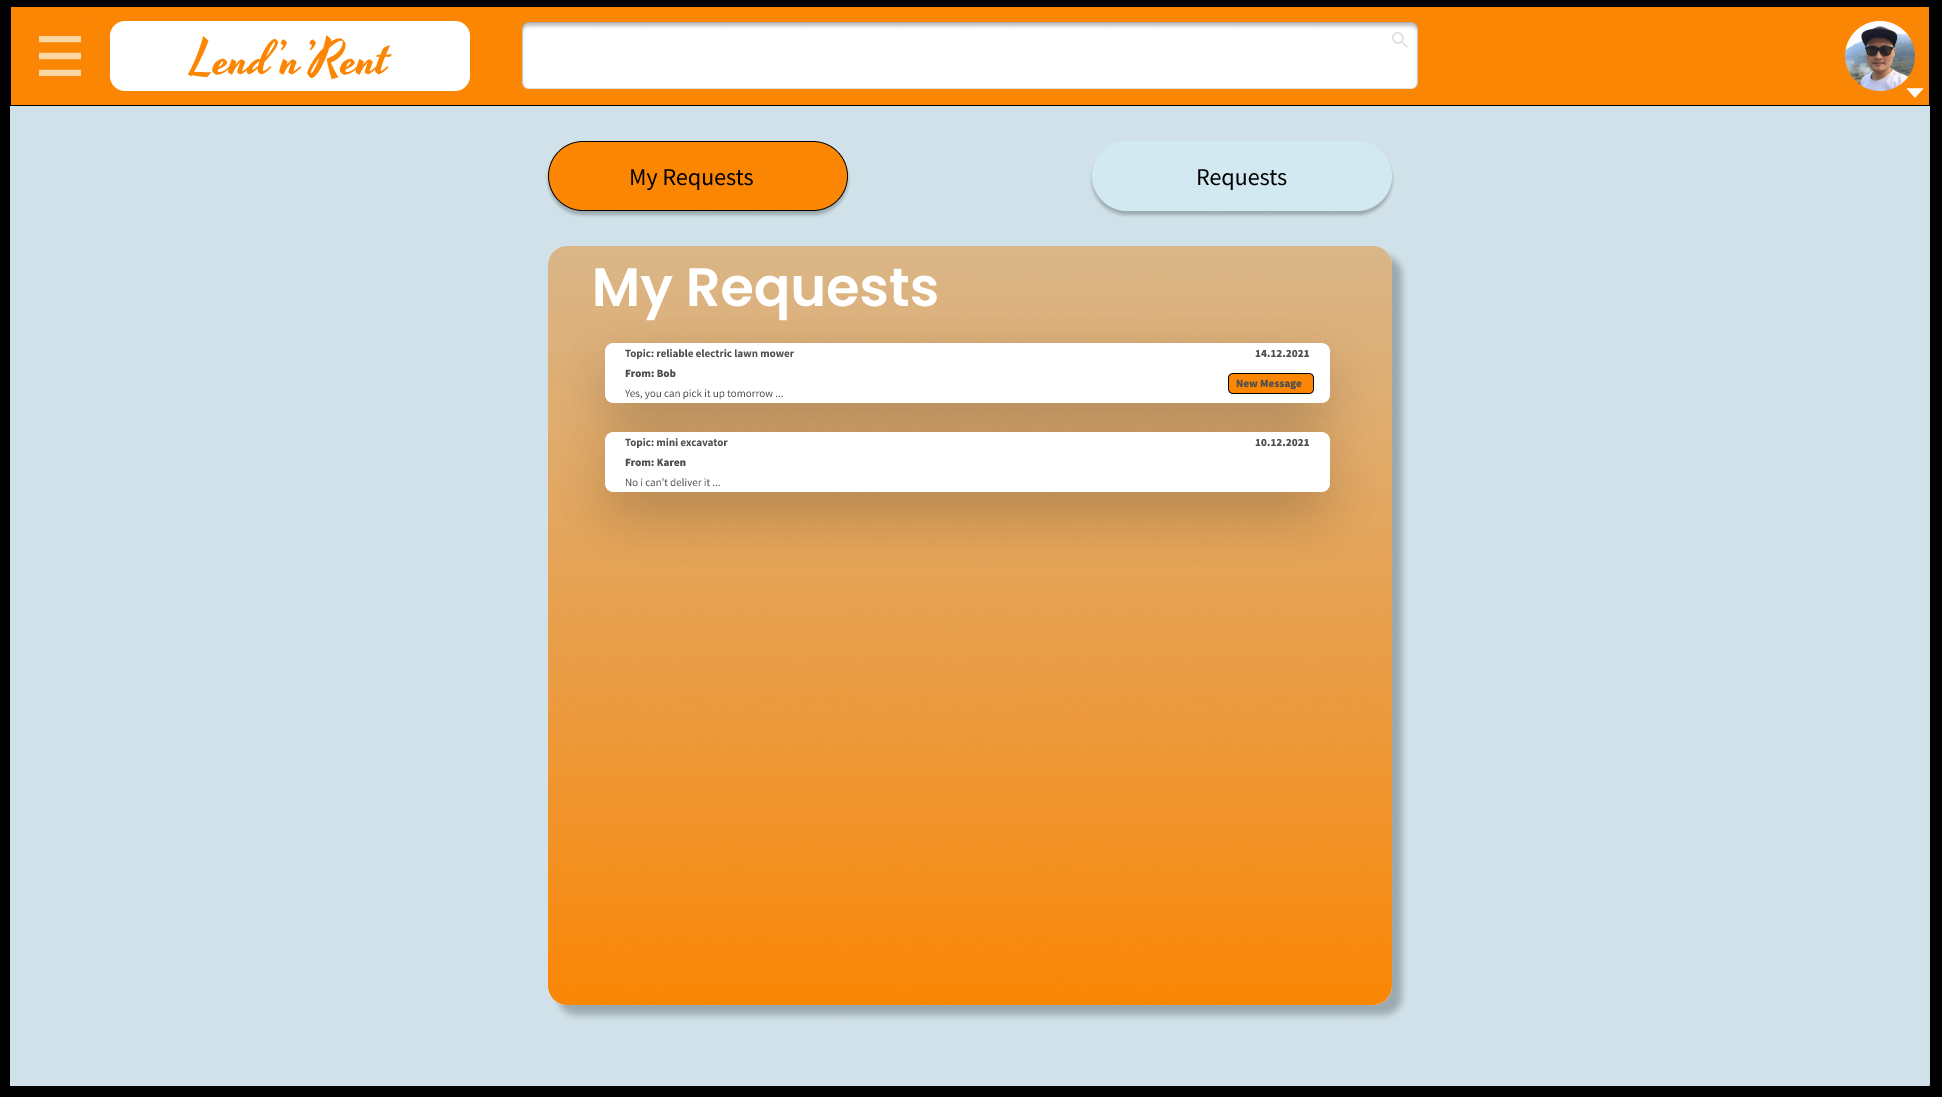
\includegraphics[width=0.49\linewidth]{abb/22chatrent}
	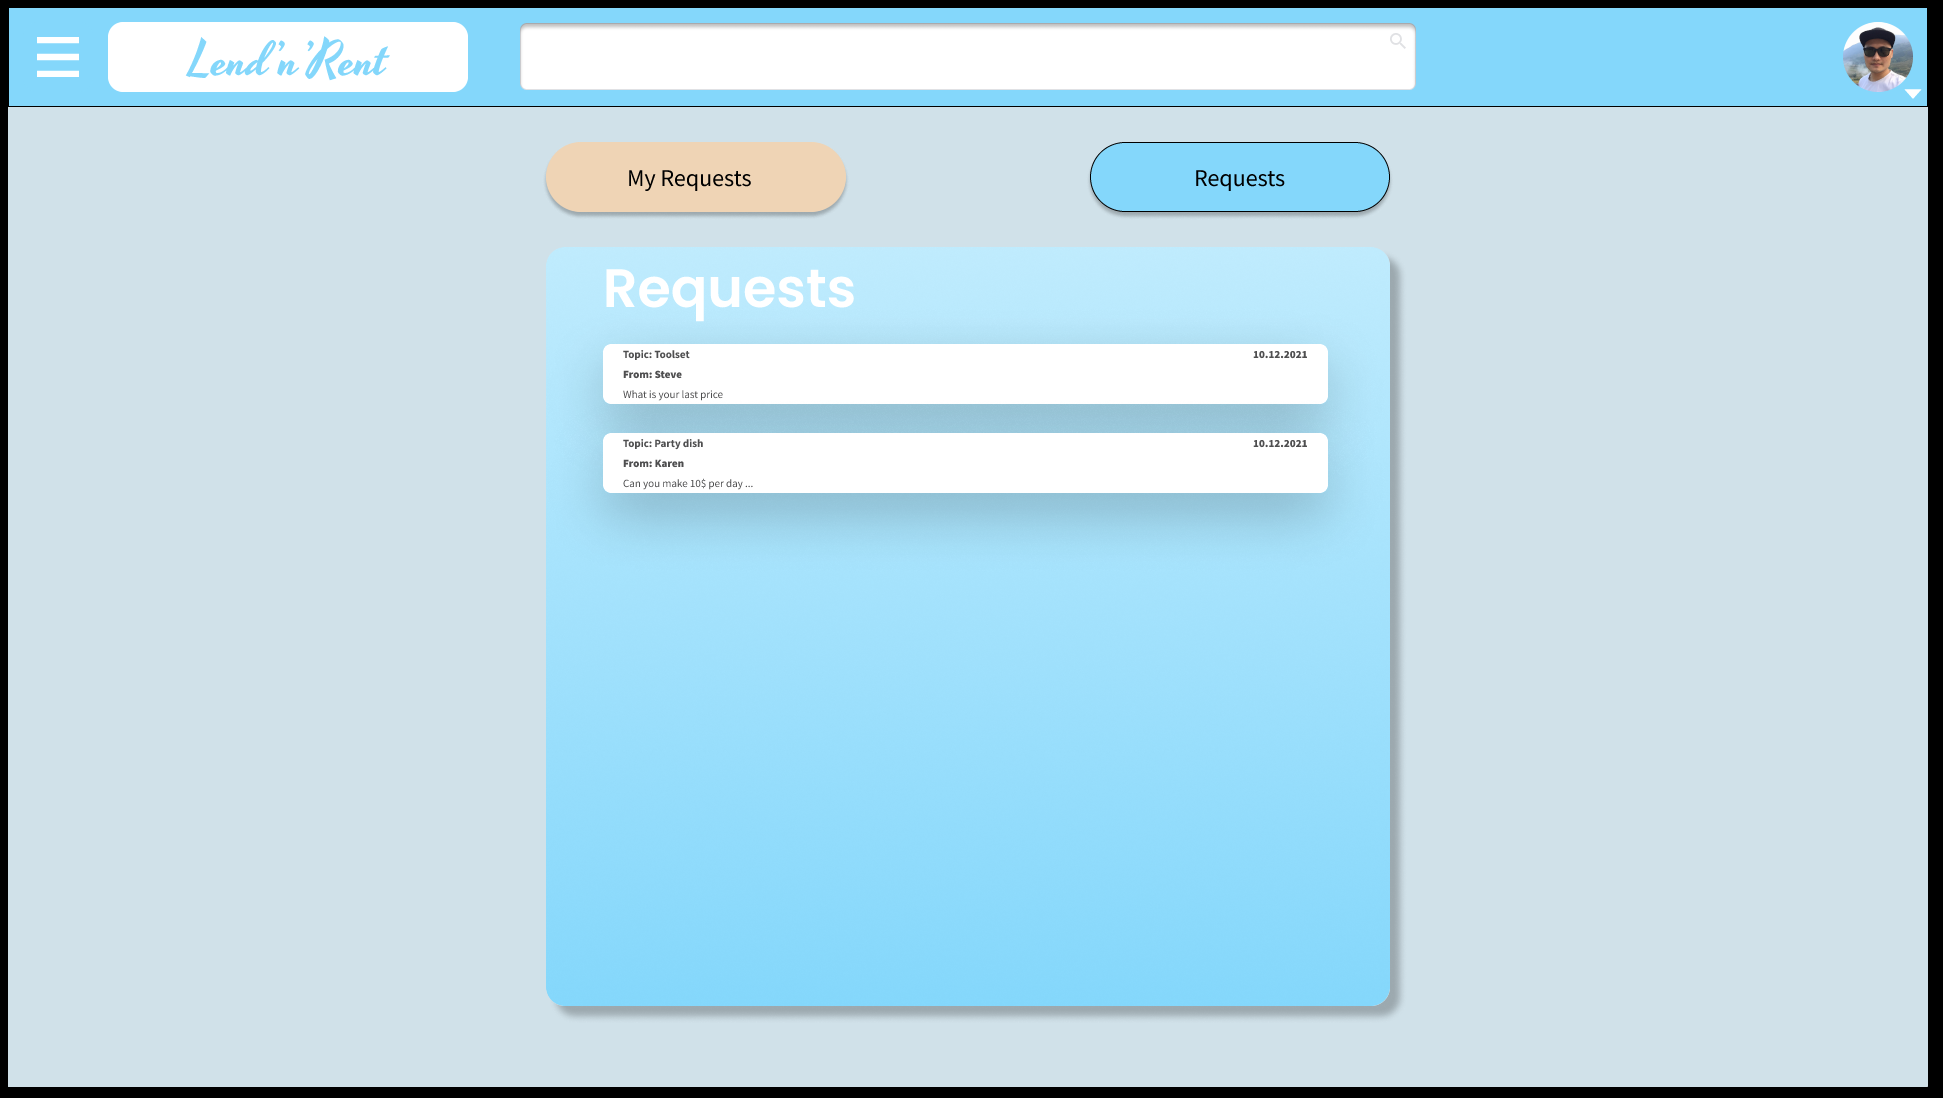
\includegraphics[width=0.49\linewidth]{abb/21chatlend}
	\caption{Messege view of lender and renter}
	\label{fig:messages}
	\centering
\end{figure}
	\newpage
	\section{Usability Guidelines}\label{Usability Guidelines}

%\subsection{Offer informative feedback}
%-

%\subsection{Match between system and the real world}
%-
%\subsection{Grant the user control and freedom}
%-
\subsection{Consistency and standards}\label{consistency}
Lend 'n' Rent provides an external consistency. \\
The searchbar is at the top in the middle of the page and the user profile is on the top right hand corner. The logo is on the top left hand corner. This arrangement can also be observed on many other websites, especially online stores. 

	\begin{figure}[H]
		\centering
		
\includegraphics[width=\linewidth]{abb/1_usability_guidelines/heuristic_constiency.png}
		\caption{consistency heuristic}
		\label{fig:heuristic_constiency}
	\end{figure}

\subsection{Support the user in avoiding errors}
When a rental transaction takes place, all agreed details must be recorded on a form. This form is prepared by the lender and must be approved by the renter. This way both parties can check all important information at a glance and misunderstandings or mistakes on both sides can be prevented. \\
	By listing the prices, the renter will not be surprised by any hidden costs.\\
		\begin{figure}[H]
		\centering
		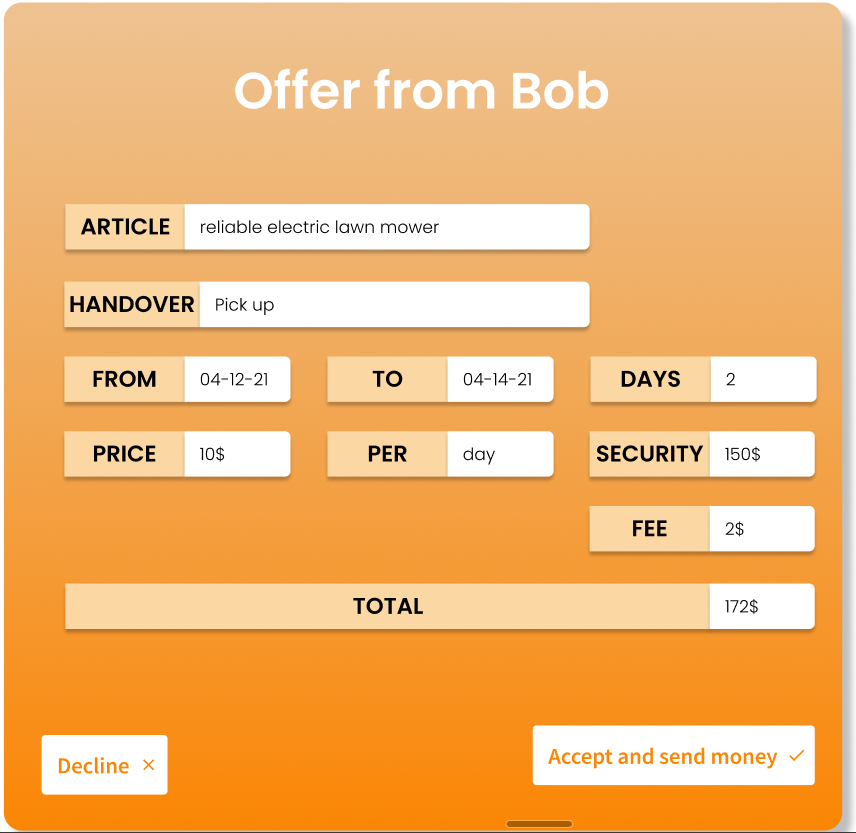
\includegraphics[width=0.7\linewidth]{abb/1_usability_guidelines/heuristic_avoid_errors.png}
		\caption{avoiding errors heuristic}
		\label{fig:heuristic_avoiding_errors}
	\end{figure}

\subsection{Minimize mental stress}
The user should be taken by the hand and guided through the entire process. The pages are kept simple and the icons are large and easy to understand. Advertising is discreetly integrated, but care is taken to ensure that it is clearly marked so that the user does not accidentally click on it. \\
All this ensures that stress and frustration are kept to a minimum.

%\subsection{Enable flexible and efficient use}
%-
%\subsection{Simple and aesthetic design}
%-
%\subsection{Allow for easy troubleshooting}
%-
%\subsection{Offer help and documentation}
%-


%\subsection{Aesthetic-Usability Effect}
%-
\subsection{Jakob's Law}
As described in section \ref{consistency}, the header is arranged exactly as it is on many other pages. This allows the user to quickly find his way around.

%\subsection{Von Restorff Effect}
%evtl die werbung ?
\subsection{Law of common region}
	\begin{wrapfigure}{l}{0.3\linewidth}
	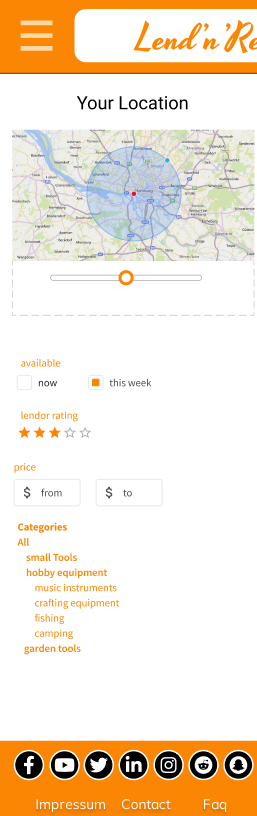
\includegraphics[width=0.3\textwidth]{abb/1_usability_guidelines/heuristic_region.png}
	\caption{Common region heuristic}
	\label{fig:heuristic_common_region}
\end{wrapfigure}
Multiple objects are displayed in a delimited region. \\
This heuristic can be observed well in the fold-out menu on the left side. In figure \ref{fig:heuristic_common_region}, for example, details of the search can be specified.



%\subsection{Fitts's Law}
%-
%\subsection{Law of Proximity}
%-
%\subsection{Pareto Principle}
%-
\subsection{Law of similarity}
Care is taken to ensure that sections are always presented in a uniform manner. On the search page, figure \ref{fig:search}, you can easily see that the articles are all of the same size and are displayed according to the same scheme.\\
 Also on the home page the categories follow a similar scheme, see figure \ref{fig:8start}. The buttons are also consistent.
%\subsection{Occam's Razor}
%-
\subsection{Law of uniform connectedness}

\definecolor{lender}{HTML}{84d7fb}
\definecolor{renter}{HTML}{fb8604}

From the beginning, the page separates by color according to the role of the user. If the user is a \textcolor{lender}{lender} , which means he has at least one item on offer, a light blue color is used. \\ If the user only borrows things, he is a \textcolor{renter}{renter} and an orange color is used. This can be seen very well on the landing page, figure \ref{fig:1landing}.


	\newpage
	\section{Evaluation}

	\newpage
	
	
	%\appendix
	%\section{Project Structure}
	%\includepdf[pages=-,offset=75 -75, scale=0.6]{app/project_structure}
	%\includepdf[pages=1, scale=0.9, frame=false]{app/project_structure}
	% einfacher Zeilenabstand
	\singlespacing
	% aturliste soll im Inhaltsverzeichnis auftauchen
	\newpage
	\phantomsection
	%\addcontentsline{toc}{section}{References}
	% Literaturverzeichnis anzeigen
	%\renewcommand\refname{Literaturverzeichnis}
	\nocite{*}
	%\bibliography{Literaturverzeichnis}{}
	
	%% Index soll Stichwortverzeichnis heissen
	% \newpage
	% % Stichwortverzeichnis soll im Inhaltsverzeichnis auftauchen
	% \addcontentsline{toc}{section}{Stichwortverzeichnis}
	% \renewcommand{\indexname}{Stichwortverzeichnis}
	% % Stichwortverzeichnis endgültig anzeigen
	% \printindex
	
	\onehalfspacing
	% evtl. Anhang
	
\end{document}
